This Chapter presents a search for dijet resonances enabled by new techniques with weak supervision.
The results of this search are published in~\cite{Aad:2020cws}.
The search does not rely on a specific signal model hypothesis and is sensitive to generic final states of the form $A\rightarrow BC$, where all of $A,B,C$ are massive and may be beyond the Standard Model, with $m_A\sim$ O(TeV) and $m_B,m_C\sim$ O(100 GeV).
The $B$ and $C$ particles are each reconstructed as single large-$R$ jets and the $A$ particle is reconstructed as a resonance in the dijet invariant mass spectrum.
The search uses a novel technique in weak supervision called classification without labels (CWoLa) to tag events with jets corresponding to possible signals with a neural network trained entirely in data.
As the first demonstration of this technique, the neural network uses a reduced set of features of just the masses of the two jets to tag potential signals.
As the neural network learns what to tag directly from data, this technique allows for avoiding the large trials factor associated with searching in the 3-dimensional feature space of $\{m_A,m_B,m_C\}$.
The search uses the full Run 2 $\sqrt{s}=13$ TeV $pp$ collisions dataset of 139\ifb{} gathered by the ATLAS detector at the LHC.
Background-only $p$-values for the dijet invariant mass between 1.8 and 8.2 TeV are reported on and no significant evidence for a localized excess is found.
In addition, new limits are set on the cross section of a variety of specific signal models with narrow-width $B,C$ decaying hadronically, with the limits ranging from 1-10 fb.
These new limits correspond to improvements of up to $10$ times existing limits from the inclusive dijet search at high $m_B,m_C$ where the inclusive dijet search is less sensitive due to that search's use of small radius jets; limits at lower values of $m_B,m_C$ where the inclusive dijet search is fully sensitive are improved by factors of up to $4$.

%-------------------------------------------------------------------------------
\section{Introduction}
\label{sec:CWoLa:intro}
%-------------------------------------------------------------------------------
One of the simplest searches that can be done at any particle collider is to look for events in which two distinct objects are formed in the detector and search for excesses in the invariant mass spectrum formed by combining these two objects.
In ATLAS the generic object formed in the detector is a jet (Chapter~\ref{ch:Jets}); almost all light standard model (SM) particles other than muons and neutrinos are reconstructed as jets in ATLAS, and more massive particles like the top quark, the vector bosons, and the Higgs boson have dominant or significant hadronic decays which are in turn reconstructed as jets, especially when boosted as is expected when decaying from a more massive resonant particle.
ATLAS has an extensive history of searches for for these \textit{inclusive} dijet resonances, including searches at $\sqrt{s}=7$~\cite{Aad:2010ae,Aad:2011aj,Aad:2011fq}, $\sqrt{s}=8$~\cite{Aad:2014aqa}, and $\sqrt{s}=13$ TeV~\cite{ATLAS:2015nsi,Aaboud:2017yvp,Aaboud:2018fzt,Aad:2019hjw}.
These searches are generically sensitive to beyond the SM (BSM) resonant decays to hadronic, electromagnetic, or electroweak objects reconstructed as jets in the detector, and therefore are one of the first searches performed when a collider reaches a new center-of-mass energy.

Dedicated searches for specific final states will always be more sensitive than the generic inclusive search, and ATLAS has an extensive program searching for di-$\tau$~\cite{Aaboud:2016cre,Aaboud:2017sjh}, di-$b$ quark resonances~\cite{Aaboud:2016nbq,Aaboud:2018tqo}, di-top quark resonances~\cite{Aaboud:2018mjh}, $bt$ resonances~\cite{Aaboud:2018juj}, di-W/Z boson resonances~\cite{Aaboud:2016okv,Aaboud:2017fgj,Aaboud:2017itg,Aaboud:2017eta,Aad:2019fbh}, VH resonances~\cite{Aaboud:2018eoy,Aaboud:2017cxo,Aaboud:2017ahz}, di-Higgs resonances~\cite{Aaboud:2018knk}, and many more.
These dedicated searches tag events based on the structure of the underlying jets in order to enhance the presence of the specific signal being searched for relative to the overwhelming background from events corresponding to SM QCD interactions.
There are also complementary searches for the direct production of BSM particles decaying into SM particles and reconstructed as a single large-$R$ jet~\cite{Aaboud:2018zba,Aaboud:2018fzt,Aaboud:2019zxd} using initial state radiation to boost the potential new particles.
Searches for any combination of SM particles can be well-motivated by one or more standard (BSM) theory frameworks~\cite{Craig:2016rqv,Kim:2019rhy}, but not all combinations are currently covered by dedicated searches.

In addition, nearly all dijet resonance searches focus on decays to SM particles.
Notable exceptions include the XH search~\cite{Aaboud:2018eoy,Aaboud:2017ecz}, where the $X$ is a $Z$-prime or $H$-like particle with unknown mass and the displaced jet search~\cite{Aaboud:2018aqj}.
Of particular relevance to this Thesis is the photon-jet search~\cite{Aaboud:2018djx} ($X\rightarrow aa, a\rightarrow \text{photons}$), with the $a$ particles boosted and reconstructed as single small-$R$ jets;
this search is sensitive to exactly the same class of models being targeted by the search presented in Chapter~\ref{ch:HBSM}, and though that search does not exactly fall under the realm of dijet searches (since the decays of the $a$ particles in that search are resolved into two separate small-$R$ jets, and the $X$ is constrained to be the Higgs boson),
future iterations of that analysis will have exactly the dijet resonance topology (Appendix~\ref{sec:HBSM_app:lowmass}).
There is currently no search for $A\rightarrow BC$, where all of $A,B,C$ can be BSM particles with possibly different masses.

This motivates the pursuit of a search which can be generically sensitive to these dijet topologies by tagging on the structure of the underlying jets which is complementary to these targeted efforts.
A meta-search consisting of an ensemble of dedicated searches for each possible signal model would suffer from a very large trials factor due to the large space of possibilities.
The trials factor accounts for the effect that since the probability of observing a large deviation from the background-only hypothesis increases with the number of orthogonal searches, a proportionally larger deviation is required from any one search in order to claim a new discovery - accounting for this effect (which is necessary) therefore makes the sensitivity of any one included search worse.

A novel analysis technique is proposed in~\cite{Collins:2018epr,Collins:2019jip} based on weak supervision approaches called classification without labels (CWoLa) first introduced in~\cite{Metodiev:2017vrx} that can be sensitive to many particular topologies all at once without paying a large trials factor.
The new technique trains a classifier directly on data, using features of the jets within events, to distinguish between events at different values of the dijet invariant mass $m_{JJ}$ which should be indistinguishable, if not for the presence of a signal resonant at one particular value of $m_{JJ}$.
Since the classifier is trained directly on data, no specific signal model hypothesis is required, and the analysis is sensitive to a wide variety of new signal models.
In addition, since the classifier is trained and tested on statistically independent datasets, there is no trials factor associated with scanning the feature space of the jets.
This intuition is explored and verified in Appendix~\ref{app:CWoLa:trials}.
The details of this technique and the application to this specific search are presented in later Sections.

This Chapter presents a search for a generic $A\rightarrow BC$ resonance where the $B$ and $C$ particles are each reconstructed as single massive large-$R$ jets, and the $A$ particle is reconstructed as a resonance in the dijet invariant mass spectrum, but other than that the properties of $A,B,C$ are not specified, and in particular may or may not be BSM.
Events collected by the ATLAS detector using the full Run 2 $\sqrt{s}=13$ TeV $pp$ collision dataset are used for the search, corresponding to 139\ifb{} of data.
The CWoLa technique is used by training a neural network to act as the classifier of potential signal.
Though the original proposal for this kind of analysis~\cite{Collins:2019jip} uses a broad class of features related to the substructure of the jet, this analysis uses a reduced feature space of just the masses $\{m_1,m_2\}$ of the two jets.
As this is the first search of its kind, this reduction is intended to simplify the analysis and understand fully all the various effects.
This simplification also allows for the setting of limits on specific signal models, since any limit setting requires the use of simulations of signal models, and the large-$R$ jet mass is well-constrained and the uncertainties are well-understood~\cite{Aaboud:2018kfi} (a similar statement cannot be made about the general substructure of large-$R$ jets).
This search is therefore essentially a search in the 3-dimensional space of $\{m_A,m_B,m_C\}$, without paying the large trials factor associated with the scan in $\{m_B,m_C\}$.

The results of this search are compared to the results from the ATLAS inclusive dijet search~\cite{Aad:2019hjw}, which as mentioned above is also generically sensitive to decays of the form $A\rightarrow \text{jets}$, but is not specifically sensitive to massive decay products of the $A$
\footnote{In fact, the incusive dijet search uses small-$R$ jets, so that the decay products of the $B$ and $C$ are not necessarily entirely contained within the jet. Because of this, as $m_B$ and $m_C$ get larger for fixed $m_A$, the limits from the incusive dijet search get worse.}.
Also relevant are the results from the ATLAS all-hadronic diboson resonance search~\cite{Aad:2019fbh}, which targets signal models of the form $A\rightarrow WW/WZ/ZZ$ and is thus sensitive to signals with $m_B\sim m_C\sim m_{W/Z}$
\footnote{In fact this analysis is expected to be considerably more sensitive to these signals, since the substructure of the jets is used in addition to the masses in order to tag the $W$ and $Z$ particles.}
, but has no sensitivity outside that range.
There are also searches for direct production of $B,C$~\cite{Aaboud:2018zba,Aaboud:2018fzt,Aaboud:2019zxd} when these are produced in association with photons or jets and their decay products are therefore collimated into a single large-$R$ jet as in this analysis.
However, those limits are orders of magnitude weaker than the ones studied here.
%$Sirunyan:2019vxa,Sirunyan:2017nvi,Sirunyan:2018ikr
This analysis does not present the limits on an exhaustive set of signal models, but rather shows the limits on a few specific models in order to demonstrate the sensitivity of the method.
For some of these signal models the limits are improved by considerable factors, up to 10 times the existing limits at high $m_B,m_C$;
for other signals, especially at low $m_B,m_C$, the technique sets about the same, worse, or no limits at all.

This Chapter is organized as follows.
First, Section~\ref{sec:CWoLa:eventsamples} introduces the data and simulated event samples.
Section~\ref{sec:CWoLa:analysis} gives a broad overview of the analysis, including the validation and blinding approach, and Section~\ref{sec:CWoLa:analysis_details} goes over the steps of the analysis in detail.
Section~\ref{sec:CWoLa:simulation_analysis} demonstrates the full analysis pipeline using dijet monte carlo to simulate the expected data.
Section~\ref{sec:CWoLa:val_analysis} demonstrates the full analysis pipeline using validation data with an inverted delta rapidity cut as a proxy for the expected data in the non-inverted signal region.
The results of the unblinded analysis are presented in Section~\ref{sec:CWoLa:unblinded}.
Finally, some aspects of the analysis, including the future outlook, are discussed in Section~\ref{sec:CWoLa:discussion} and the conclusions are provided in Section~\ref{sec:CWoLa:conclusion}.

\section{Event Samples}
\label{sec:CWoLa:eventsamples}

%The \href{https://gitlab.cern.ch/atlas/athena/blob/master/PhysicsAnalysis/DerivationFramework/DerivationFrameworkExotics/share/EXOT3.py}{EXOT3} derivation is used for both data and simulation.  ATHENA release 21 is used throughout. 

\subsection{Data}
\label{sec:CWoLa:data}

This analysis is performed using data from $pp$ collisions provided from the Large Hadron Collider with $\sqrt{s} = 13$~\TeV~between 2015-2018, and collected with the ATLAS detector. The total integrated luminosity of this dataset is 139~\ifb.

Data are collected using the lowest available unprescaled single large-radius jet trigger, which varies depending on the period during Run 2.
In all years, the Level 1 trigger require a Level 1 jet with $\pt>100$ GeV (\texttt{L1\_J100}).
In 2015 and 2016 the triggers in the high-level trigger fire on the untrimmed jet $\pt$; in 2015 the requirement was $360$ GeV (\texttt{HLT\_j360\_a10\_lcw\_sub\_L1J100}), and in 2016 this requirement was raised to $420$ GeV (\texttt{HLT\_j420\_a10\_lcw\_L1J100}).
From 2017 onward, the triggers in the high-level trigger use the trimmed jet $\pt$ and apply a jet energy scale calibration, and the requirement on this $\pt$ was $460$ GeV (\texttt{HLT\_j460\_a10t\_lcw\_jes\_L1J100}).
%\footnote{This is the same as the all-hadronic diboson resonance search and the text here is copied from their support note~\cite{Aad:2019fbh}.}

\subsection{Simulation}

As will be described in Section~\ref{sec:CWoLa:analysis}, this analysis is completely data-driven, both for training and testing.
However, simulations of the expected background are used to validate the procedure and simulations of signals are used for setting model-dependent limits.
Samples of Monte Carlo (MC) simulated dijet and multijet events are used to emulate the SM (Section~\ref{sec:ATLAS:simulation}).
As the jet cross-section is orders of magnitude larger than electroweak processes, the consideration of these samples is sufficient to describe the data and all other processes are ignored.  

\PYTHIA{} v8.2~\cite{Sjostrand:2007gs,Sjostrand:2006za} is used as the nominal MC generator for this analysis.
Samples of $2\rightarrow 2$ dijet events are simulated using the A14 tune~\cite{ATL-PHYS-PUB-2014-021} and NNPDF 2.3~\cite{Ball:2012cx} parton distribution function (PDF) set.
The after-burner generator EvtGen~\cite{Lange:2001uf} is used to model decays of heavy flavor hadrons.
In order to fully populate a wide range of jet \pt, these samples are generated in slices of the particle-level $R=0.6$ jet \pt.
%Two alternative samples are generated with the \SHERPA{} v2.1~\cite{Gleisberg:2008ta} and \HERWIG{} v7.0.4~\cite{Bahr:2008pv,,Bellm:2015jjp} generators. The \HERWIG{} v7.0.4 sample is generated with the NNPDF 3.0 NLO PDF set and using the H7UE~\cite{Bellm:2015jjp} set of tuned parameters. The \SHERPA{} v2.1 leading-order multileg samples use the CT10 PDF set~\cite{Lai:2010vv} and are generated with the default \SHERPA{} tune and include $2\rightarrow 2$ and $2\rightarrow3$ processes at matrix element level, combined using the CKKW prescription~\cite{Catani:2001cc}.

%\href{https://its.cern.ch/jira/browse/ATLMCPROD-6767}{Signal samples are generated} using \PYTHIA{} v8.2 and the process $Z'\rightarrow WZ$, where the $W$ and $Z$ masses are altered, the widths are set to 0.1 GeV.
Signal samples are generated using \PYTHIA{} v8.2 and the process $Z'\rightarrow WZ$, where the $W$ and $Z$ masses are altered, and their widths are set to 0.1 GeV.
These altered bosons are required to decay hadronically, except that top quark decays are switched off.
As the parameter space of this simplified model is three-dimensional, we consider only a subset of all possibilities in order to demonstrate the method on some example signal models.
The samples shown for the rest of this Chapter use $m_{Z'}\in\{3,5\}$~TeV and $\{m_W,m_Z\}\in\{80,200,400\}$~GeV.

All simulation is reconstructed using a full detector simulation and superimpose simulated minimum-bias interactions to represent multiple $pp$ interactions during the same or nearby bunch crossings (pile-up).
The distribution of the average number of pile-up interactions in simulation is re-weighted during data analysis to match that observed in the Run 2 data.

%Lists of the specific MC samples used for this analysis are provided in Appendix~\ref{sec:CWoLa:app:CWoLa:samples}.

\FloatBarrier
%-------------------------------------------------------------------------------
\section{Analysis Overview}
\label{sec:CWoLa:analysis}
%-------------------------------------------------------------------------------

\subsection{Background: CWoLa and CWoLa Hunting}
\label{sec:CWoLa:schematic}
In a typical search for BSM at the LHC, some particular signal model is designated and an event selection is optimized to target this signal relative to the expected background using signal simulation and some proxy for the background (either simulation- or data-based).
This is for example the strategy pursued in the search presented in Chapter~\ref{ch:HBSM}, in which the event selection was chosen roughly manually to optimize the signal to background discrimination power.
This strategy is also employed for example by the all-hadronic diboson resonance search~\cite{Aad:2019fbh}, where dedicated $W/Z$ hadronic jet taggers are trained as somewhat of a black box on simulation; the tagger is then calibrated in data, using a high-fidelity sample of $W/Z$ jets (e.g. from $t\bar{t}$ events where one of the daughter $W$ particles decays leptonically) to compare and correct the difference in estimated efficiency on $W/Z$ jets in simulation and in data.
This method of tagging signal can be broadly classified as ``supervised learning'', since the tagger is told what is signal and what is background at time of training.

There are two major drawbacks related to training a classifier in simulation and using it in data.
First, the simulation of the signal may not itself be entirely accurate, leading to a suboptimal selection even on the specific signal model in data.
Data/simulation calibrations can remove bias in the tagger, in the sense that the efficiency on signal events estimated in simulation can be corrected to the efficiency estimated in data, but they do not in general remove this suboptimality\footnote{E.g., consider a case where a $W$ jet tagger is being trained in simulation using the jet mass as a feature. Suppose further that the $W$ jet mass is centered at $80$ \GeV{} in simulation but at $70$ \GeV{} in data (of course the jet mass is itself calibrated between data and simulation so this would not be the case, but the dedicated $W/Z$ taggers do use certain features which are not themselves calibrated, and the jet mass is used as a simple tangible example feature to demonstrate the point). Then the tagger trained in simulation might derive an optimal selection centered around $80$ \GeV{}. When calibrating, the efficiency measured in simulation would be corrected to the actual efficiency in data on $W$ jets with that selection, but the simulation-trained tagger would never find the true optimal selection, which would be centered around $70$ \GeV{}.}.
Second, the trained tagger will only be sensitive to the specific signal model used for training, limiting sensitivity to other similar signals but with different values of the features used in training.
There is therefore a motivation to train a classifier directly on data to tag whatever signals that may be found there.

There is of course the obvious issue that in data there are no labels on individual events telling the tagger whether the event comes from a signal or background process.
However, a series of techniques using ``weakly supervised learning'' have been developed for high energy physics, which allow for learning even when these per-instance labels are not present~\cite{Metodiev:2017vrx,Dery:2017fap,Cohen:2017exh,Komiske:2018oaa}.
The basic idea for this method is shown in Figure~\ref{fig:CWoLa:cwolasetup}.
The setup of CWoLa is that there are two samples, each of which has a mixed composition of signal and background events.
Crucially, the fraction of signal and background events between the two samples must be different; and while of course the signal and background events must differ from each other in the distributions of some features, the signal events and background events cannot differ among themselves between the two samples
\footnote{
Or rather, if there are differences between background events in Mixed Sample 1 and background events in Mixed Sample 2, those differences must be smaller than the difference in signal fraction between the two samples times the difference between signal and background.  
}.
The insight of the CWoLa method is that a classifier can be trained to distinguish between the two mixed samples using any supervised learning technique.
The resulting classifier learns to distinguish between the signal and background events.
The main result of~\cite{Metodiev:2017vrx} is that it can be proved that this procedure produces an optimal classifier for distinguishing signal from background in the asymptotic limit (enough data, flexible enough training model, etc.).

\begin{figure}
\centering
\includegraphics[width=0.6\textwidth]{figures_CWoLa/cwola_nokoala.png}
\caption{
  Schematic of basic idea behind classification without labels (CWoLa).
  There are two samples, each of which has a mixed but different composition of signal and background events.
  A supervised classifier is trained to distinguish between the two mixed samples.
  This same classifier is then used to distinguish between signal and background events.
  Figure sourced from~\cite{Metodiev:2017vrx}.
}
\label{fig:CWoLa:cwolasetup}
\end{figure}

It is worth noting the properties and limitations of this method.
First, the features used to distinguish between signal and background events cannot or can only be very bad at distinguishing between background events in Mixed Sample 1 and Mixed Sample 2 (and similarly for signal events, though typically the signal presence is very small in one sample and basically zero in the other, so this is not as much of a concern).
Second, the key insight is that it is okay if there is some signal in both mixed samples; however, learning is easiest when the fraction of signal between the two mixed samples differs the most.

Because the classifier is trained directly on data, it avoids the first major drawback of supervised learning mentioned above, since there is no possible simulation-data difference, either in the signal events or in the background events.

As mentioned above, the second major limitation of supervised learning is that the trained classifier is only sensitive to one particular signal model, preventing the application to a generic search like the one being discussed here.
The idea of ``CWoLa hunting''~\cite{Collins:2018epr,Collins:2019jip} is to use the CWoLa method to search for BSM physics without a particular signal model in mind, enabling a generic search for new physics.
In fact, the method learns to tag whatever signal is present in the data, allowing the search to be generically sensitive to new signals that have different distributions of whatever features are used than the background.

The setup CWoLa hunting is shown schematically in Figure~\ref{fig:CWoLa:cwolahuntingsetup}.
There is some feature $m_\text{res}$ for which the background has a smoothly falling spectrum, while the signal is narrowly peaked (\textit{resonant}) in that feature.
Two mixed samples are formed: one with values of $m_\text{res}$ centered near the potential new resonance and one using events in neighboring regions of $m_\text{res}$.
A neural network is trained to distinguish between these two mixed samples based on some other features, resulting in an overall score $y$.
The first mixed sample clearly has a higher signal fraction than the second;
and because the two mixed samples come from nearby regions of $m_\text{res}$, the difference in distributions of features in the background between the two mixed samples can be smaller than the fraction of signal times the difference in distributions between the signal and background.
Therefore, because of the principles of CWoLa, the scores from the resulting network $y$ can distinguish between signal and background events. 
In the case that in fact there was no signal in the first mixed sample, the tagger will either learn to tag randomly or learn to tag based on the minute differences in the background between the samples.
In either case, after tagging based on the output $y$, the combined spectrum of $m_\text{res}$ can be fit with a smooth function - if indeed there was a signal, there will be a bump in the $m_\text{res}$ spectrum; while if there was no signal, the background should remain smooth, even if the network learned to tag some differences in the background\footnote{This is why it is key to use neighboring regions on both sides. The prevention of background sculpting is a major consideration in this analysis, as discussed in more detail in Section~\ref{sec:CWoLa:Analysis:Overview}.}.
This process is then repeated for different regions of $m_\text{res}$ in order to be sensitive to a broad spectrum of BSM masses.
One of the key aspects of this technique is a nested cross-validation procedure, which prevents overtraining in the case of no signal presence.

\begin{figure}
\centering
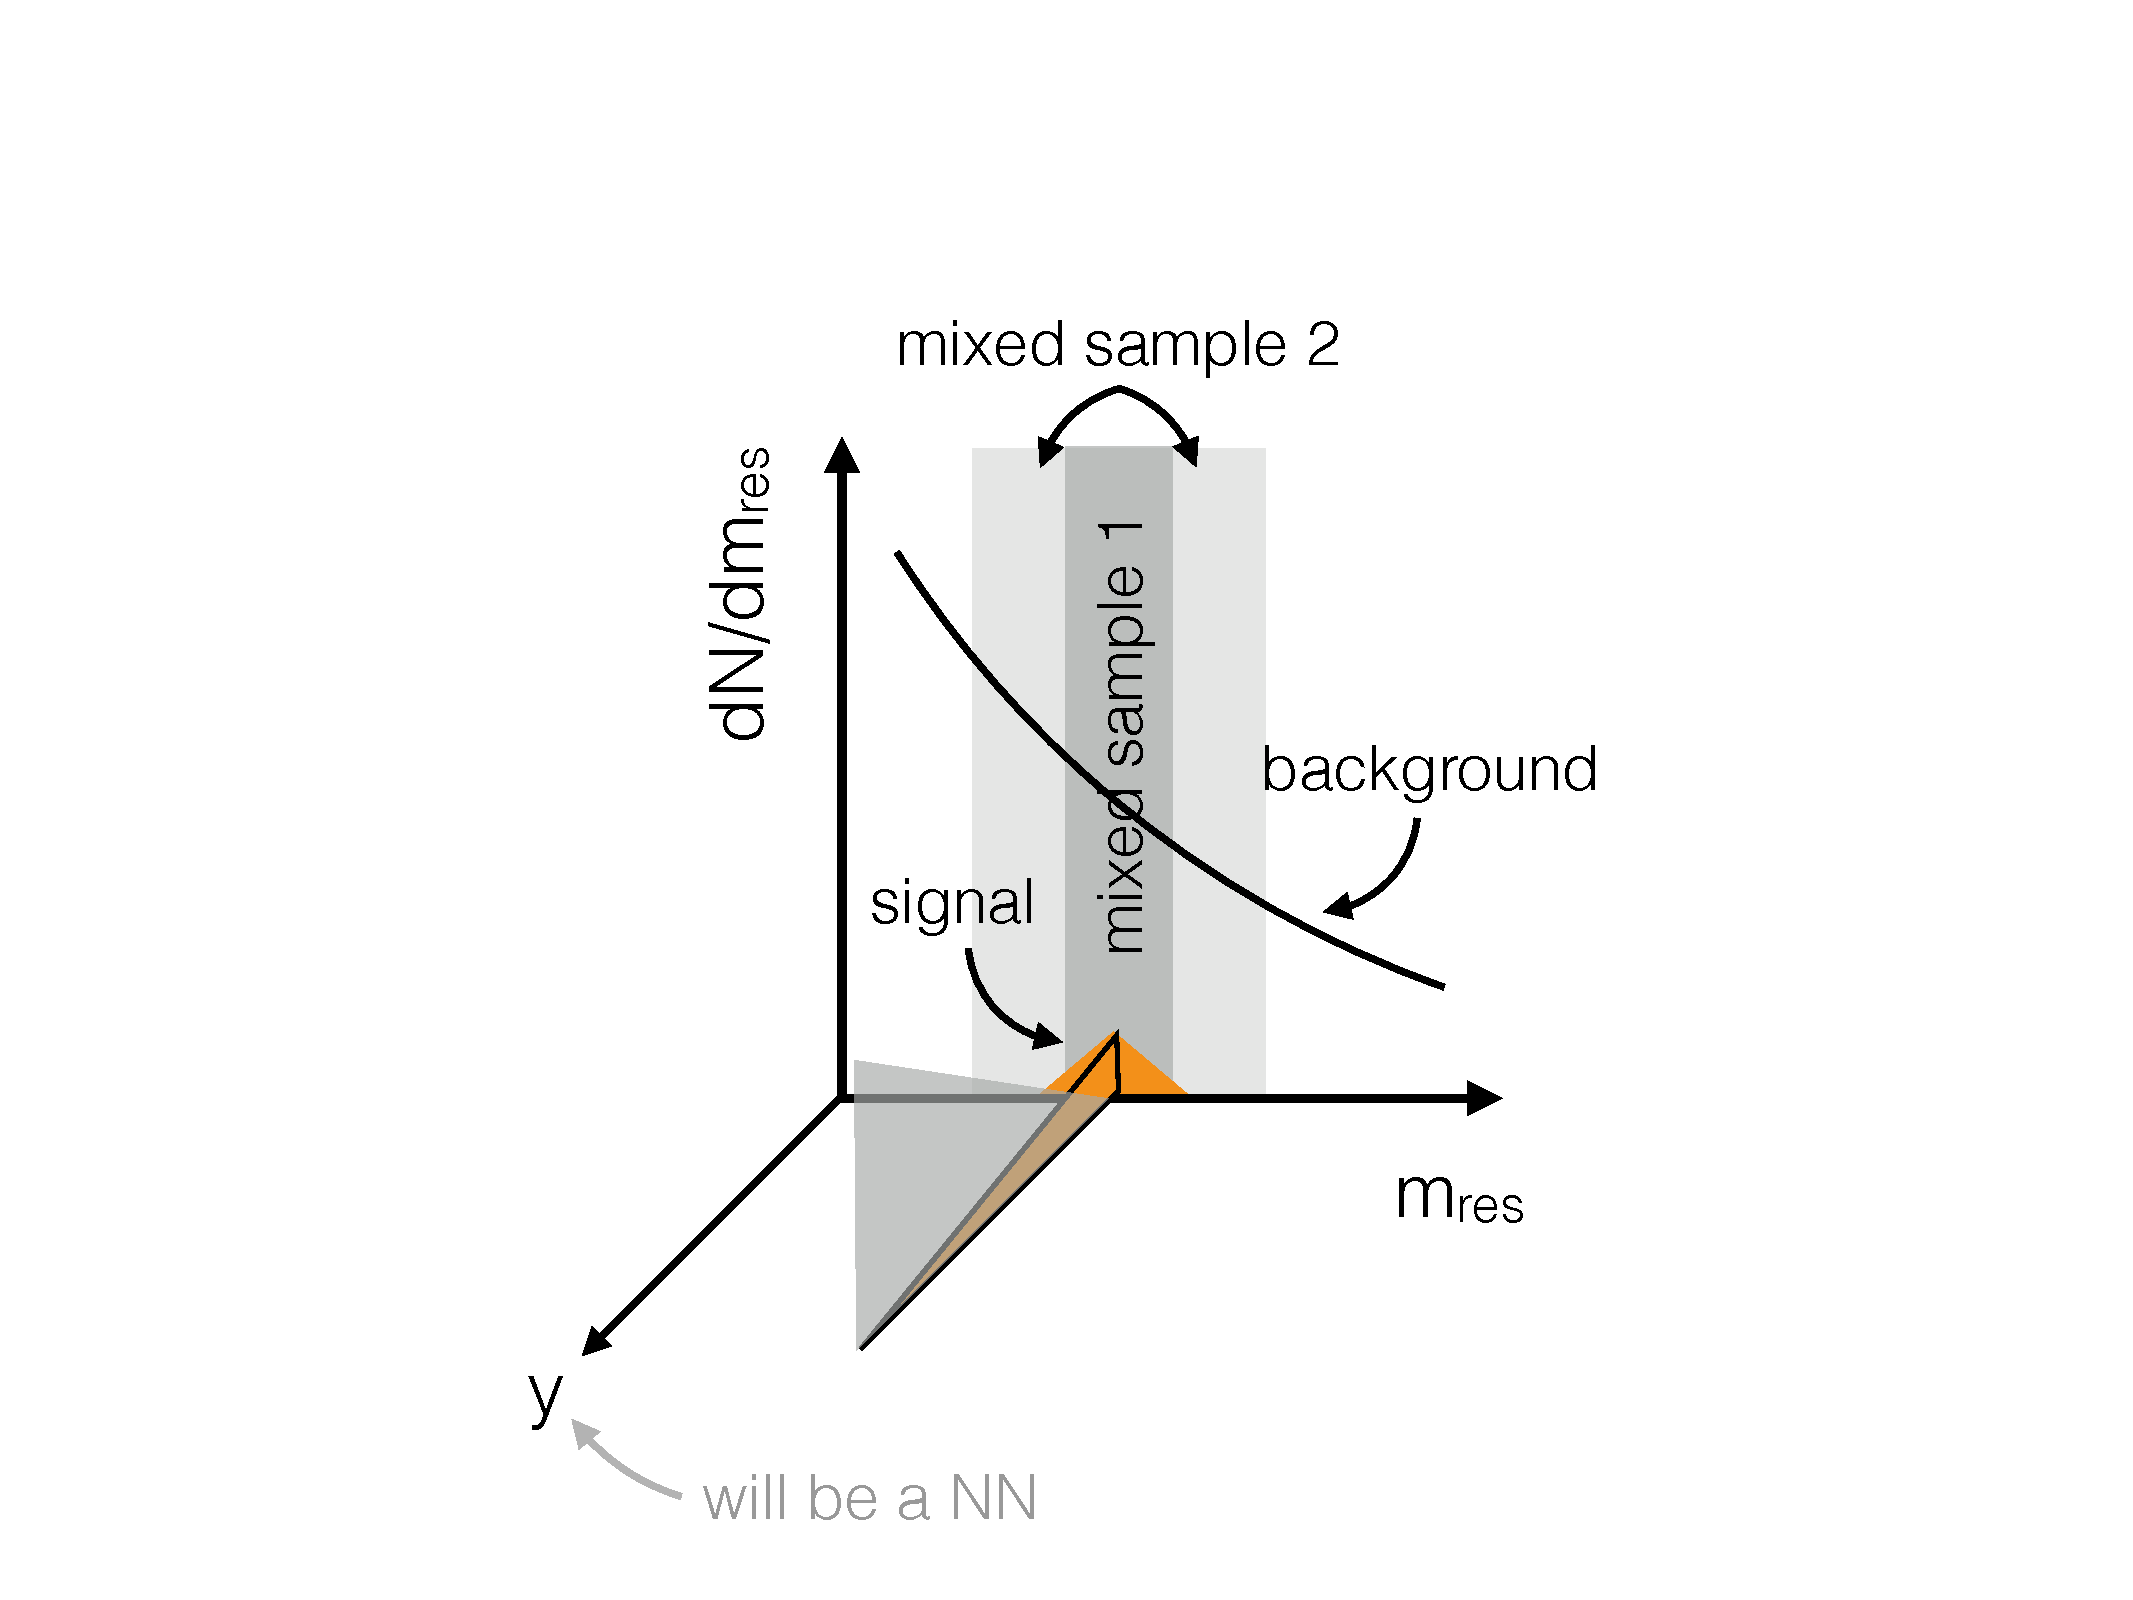
\includegraphics[width=0.5\textwidth]{figures_CWoLa/cwolahuntingsetup.pdf}
\caption{
  A schematic for the setup of CWoLa hunting.
  The background has a smoothly falling spectrum in some feature $m_\text{res}$, while the signal is narrowly peaked (resonant) in that feature.
  A network is trained to distinguish between a narrow region of $m_\text{res}$ in which the signal lies from its neighboring regions.
  Because of the principles of CWoLa, the scores from the resulting network $y$ can distinguish between signal and background events. 
  Figure adapted from~\cite{NPKI_CWoLa_Hunting}.
}
\label{fig:CWoLa:cwolahuntingsetup}
\end{figure}

This and other key aspects are discussed in the following Section (\ref{sec:CWoLa:Analysis:Overview}), which lays out the assumptions and specifics of this analysis based on the above ideas with $m_\text{res}=m_{JJ}$.

It should be noted that CWoLa hunting is not the only possible way of doing a model-independent bump hunt.
A broad classification of existing and proposed searches based on their signal and background model independence is shown in Figure~\ref{fig:CWoLa:ANODE}.
As mentioned above, many analyses train a tagger to distinguish between signal and background simulations, and these analyses are therefore dependent on both signal and background modeling.
There are a few analyses which train a tagger to distinguish between signal simulations and unlabeled data and are therefore background model independent, e.g. in the $\gamma\gamma$ channel of the observation of $t\bar{t}H$~\cite{Aaboud:2018urx}, using a validation region with low signal efficiency as the background sample for training.
There are also some searches which directly test the compatibility of the observed data with the background-only hypothesis in a portmanteau test by comparing the observed data directly to the simulation of the background in ATLAS~\cite{ATLAS-CONF-2012-107,ATLAS-CONF-2014-006,Aaboud:2018ufy} and in CMS~\cite{CMS:2011fra,CMS:2017yoc}; these searches are therefore signal model independent but heavily dependent on background modeling.
Recently, there have been proposals to enhance these searches with deep learning~\cite{DAgnolo:2018cun,DAgnolo:2019vbw}.

CWoLa hunting falls into a final category which is both signal and background modeling independent.
There are a few direct competitors to CWoLa hunting which also have these model independent properties.
Many of these searches are based on autoencoders~\cite{Farina:2018fyg,Heimel:2018mkt,Roy:2019jae,Cerri:2018anq,Blance:2019ibf,Hajer:2018kqm}, but there are other unsupervised techniques based on nearest neighbor classification~\cite{1809.02977,DeSimone:2018efk,Mullin:2019mmh}, probabilistic modeling~\cite{Dillon:2019cqt}, reweighted simulation~\cite{Andreassen:2020nkr}, density estimation~\cite{Nachman:2020lpy}, and others~\cite{Aguilar-Saavedra:2017rzt}.
These techniques must also be combined with a background estimation strategy, either in the form of a bump hunt, or using simulation, similarly to CWoLa hunting.
The main difference between these techniques and CWoLa hunting is that they are \textit{un}supervised, while CWoLa hunting is \textit{weakly} supervised.
I.e., the unsupervised methods simply find natural groupings or patterns in the data, and it may be the case that a new signal does not fit into those groupings or follow those patterns so that the unsupervised network can tag these as anomalies (however such an outcome is not guaranteed).
The weakly supervised method, on the other hand, does see the signal during its training, if it exists, and so therefore can be biased towards better tagging the signal.
Because of this difference, when signal rates are large enough such that the weakly supervised network can learn some information to tag the signal itself, the weak supervision method is superior.
On the other hand, the unsupervised approaches can do better when there is very little signal.

\begin{figure}
\centering
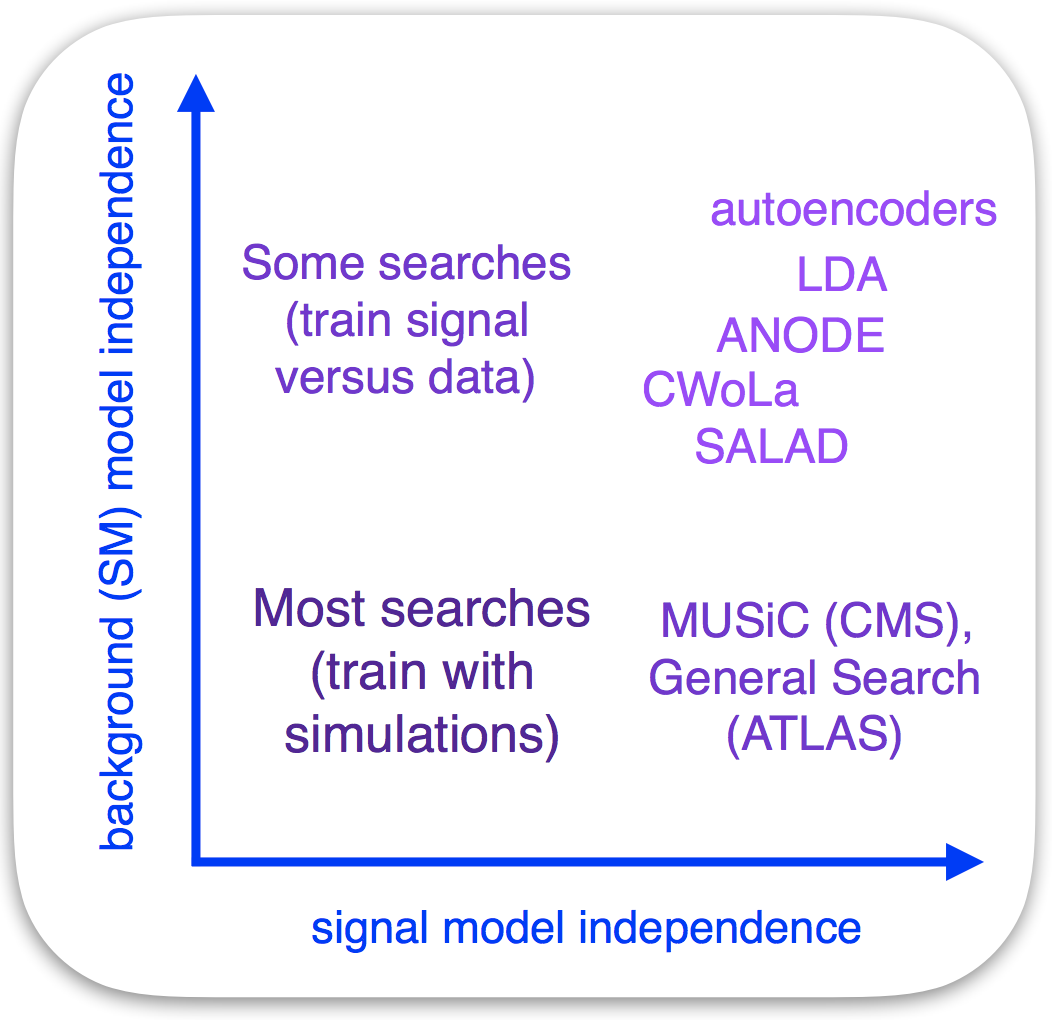
\includegraphics[width=0.5\textwidth]{figures_CWoLa/ANODE.png}
\caption{
  Classification of existing and proposed searches based on their signal and background model independence.
  The MUSiC (Model Unspecific Search for new physiCs)~\cite{CMS:2011fra,CMS:2017yoc} and General Search~\cite{ATLAS-CONF-2012-107,ATLAS-CONF-2014-006,Aaboud:2018ufy} are used in CMS and ATLAS, respectively.
  Methods based on autoencoders~\cite{Farina:2018fyg,Heimel:2018mkt,Roy:2019jae,Cerri:2018anq,Blance:2019ibf,Hajer:2018kqm}, LDA (Latent Dirichlet Allocation)~\cite{Dillon:2019cqt}, ANODE (ANOmaly detection with Density Estimation)~\cite{Nachman:2020lpy}, and SALAD (Simulation Assisted Likelihood-free Anomaly Detection)~\cite{Andreassen:2020nkr} can be considered to be direct competitors to CWoLa~\cite{Metodiev:2017vrx,Collins:2018epr,Collins:2019jip}.
  Figure sourced from~\cite{Nachman:2020lpy}.
}
\label{fig:CWoLa:ANODE}
\end{figure}

It is important to point out that, while CWoLa hunting can be sensitive to a broad set of signal models, there are some assumptions made about the signal so that the method is not totally generic.
First, there is an assumption that the signal is resonant in $m_\text{res}$, preventing sensitivity to wide or non-resonant signals.
Second, there is a requirement that there are features of the signal events that can distinguish them from the background other than $m_\text{res}$ (although if this were not the case the best search that could be done would be the inclusive fit in $m_\text{res}$, as there is no signal/background discrimination power).
Third, as will be mentioned in Section~\ref{sec:CWoLa:blinding}, for the specific search using CWoLa hunting discussed here (with $m_\text{res}=m_{JJ}$), a non-trivial selection is placed on the rapidity difference between the two jets.
This selection basically amounts to an assumption that the $A\rightarrow BC$ process being targeted by this search occurs via an $s$-channel process, and removes a large amount of the background due to $t$-channel QCD processes.
It should be noted that this selection is also applied in the inclusive dijet search~\cite{Aad:2019hjw} and in the all-hadronic diboson resonance search~\cite{Aad:2019fbh}, which are sensitive to similar signals and also aim to be inclusive in their sensitivity.

The search presented here, using CWoLa hunting with $m_\text{res}=m_{JJ}$, is the first application of these model-independent generic searches with LHC data.

\FloatBarrier
\subsection{Analysis Strategy}
\label{sec:CWoLa:Analysis:Overview}
This analysis utilizes the concept of Classification Without Labels (CWoLa) described in Section~\ref{sec:CWoLa:schematic} in order to be sensitive to a broad class of non-SM models of the form $A\rightarrow BC$, with $A$ massive and on-shell, and the decay products of $B$ and $C$ reconstructed as large-$R$ jets in the ATLAS calorimeter.
In these models, the reconstructed dijet mass $m_{JJ}$ will show a peak near the mass of the $A$, with width determined by the dijet mass resolution.
There are two key assumptions that enable this analysis to be sensitive to these models.
\begin{enumerate}
  \item \textbf{(Assumption 1)} One or both of the jets reconstructed from the $B$ and $C$ decays have features, e.g. in their substructure, which differ from the background composition (i.e., non-resonant dijet events from QCD and other SM processes), so that these jets can be tagged in order to increase the signal to background ratio of the signal $m_{JJ}$ peak over the background shape. \label{ass1}
  \item \textbf{(Assumption 2)} After tagging on these features, the background $m_{JJ}$ remains smooth, so that a fit to the background $m_{JJ}$ spectrum does not indicate a potential discovery via a bump in the $m_{JJ}$ spectrum. \label{ass2}
\end{enumerate}
In particular, clearly one of the features that differs between the signal and the background composition is $m_{JJ}$ itself; if $m_{JJ}$ is used as a feature, or if jet features that allow reconstruction of $m_{JJ}$ are used, then Assumption~\ref{ass2} is violated, because after tagging on this feature the $m_{JJ}$ spectrum in the background will no longer be smooth.
Therefore some effort must be put into choosing features that will not violate Assumption~\ref{ass2}, and into validating that the assumption is not violated once the features are chosen.

Under these assumptions, the outline of the analysis is as follows.
\begin{enumerate}
  \item Select events in which at least two large-$R$ jets are reconstructed, and in these events form the dijet invariant mass, $m_{JJ}$, and record some relevant jet features $X$.\label{step1}
  \item Partition the $m_{JJ}$ spectrum into discrete, monotonically increasing bins.\label{step2}
  \item Label one of these bins the \textit{signal region}, and the bins on either side in $m_{JJ}$ space the \textit{sideband regions}.~\label{step3}
  \item Train a neural network (NN) to distinguish between the signal region and the sideband regions based on the chosen features $X$.
    There are three possibilities of what the network learns, based on where the true signal lies relative to the signal region.
    \begin{enumerate}
      \item If the signal mass peak happens to lie in the signal region, then the signal fraction in the signal region will be higher than in the sideband regions, and the network will learn that it can identify some events in the signal region by tagging the true signal; i.e., the network will learn how to tag signal events.
        This process is what is referred to as CWoLa.\label{case1}
      \item If the signal mass peak happens to lie in one of the sideband regions, then the signal fraction in the signal region will be lower than in the sideband regions, and the network will learn to identify some events in the sideband region by tagging the true signal; i.e., the network will learn how to anti-tag signal events.\label{case2}
      \item If the signal mass peak does not lie in the signal region or sideband regions, or if there is no signal at all, then the network will learn to distinguish between the background events in the signal and sideband regions based on the features $X$, as far as such correlations exist.\label{case3}
    \end{enumerate}
    Note that, in Cases~\ref{case1} and~\ref{case2}, the network is sensitive to both the difference in the distribution of the features $X$ between the signal and the background, and to the differences between the background in the signal region and the background in the sideband regions.
    In order to allow the network to focus on tagging the signal versus the background, the sideband regions are chosen to be adjacent to the signal region in kinematic space so that the difference in the features in the background between the signal and sideband regions is minimzed.
  \label{step4}
  \item Tag events by choosing events with high neural network output.
    In Case~\ref{case1}, the neural network is a signal tagger, so the signal-to-background ratio increases, in particular increasing the significance of the signal peak over the background $m_{JJ}$ shape. 
    In Case~\ref{case2}, the network anti-tags signal, and in Case~\ref{case3}, the network tags only differences in the background between signal and sideband regions; in either case, the signal-to-background ratio after tagging is small or zero.
  \label{step5}
  \item Fit to the $m_{JJ}$ shape after tagging.
    Because of Assumption~\ref{ass2}, the background spectrum is smooth after tagging.
    In Case~\ref{case1}, there will be a bump in the $m_{JJ}$ spectrum in the signal region due to the presence of signal, allowing the potential of a discovery of this signal.
    In Cases~\ref{case2} and~\ref{case3}, there will be little to no signal, so there will be no bump in the $m_{JJ}$ spectrum, and the spectrum fit will not indicate the discovery of a signal.
    \label{step6}
  \item Repeat Steps~\ref{step3}-\ref{step6} with each possible signal region bin.
    If there is any true signal, then the signal will lie in one of the signal region bins, and Case~\ref{case1} will be true in that bin, allowing discovery of this signal.
    If there is no true signal, then in each signal region bin Case~\ref{case3} will be true, thus indicating no discovery over the whole $m_{JJ}$ range.
\end{enumerate}
Since there is a difference in the observed outcomes between the case where there is presence of signal and when there is no signal, limits can be set on specific signal models based on what would have been observed if those signals were present.

Since the network learns what features distinguish the signal from the background automatically, this analysis is sensitive to a wide range of possible signal distributions of these features, and thus the analysis can be sensitive to a wide range of signal models without paying the price of a trials factor that a dedicated search for each one of these signal models would entail.

Furthermore, since the network learns the features that distinguish the signal from the background directly from data, the tagger does not suffer from suboptimality due to differences between simulation and background, as could be the case with a tagger trained to distinguish between signal and background in simulation.

\FloatBarrier
\subsection{Blinding and Validation Procedure}
\label{sec:CWoLa:blinding}
Validating the analysis in a blinded region of the data is a challenge for this analysis.
In a typical analysis, after running the analysis entirely in simulation, some validation region is defined with orthogonal cuts with low signal efficiency in order to validate the analysis.
This validation region is used to either do data/MC comparisons to verify that the simulation is describing the background adequately or to perform in situ checks of the assumptions of the analysis.
For example, in the search described in Chapter~\ref{ch:HBSM}, the background is estimated in a data-driven way with an A/B/C/D matrix of regions; the highest signal efficiency is expected in region D.
The assumption of the A/B/C/D method (that the ratio of events in B/A is the same as in D/C in the background) is verified both in simulations of the background and in a data validation region, inverting the $m_{gg\gamma\gamma}$ cut.

In this analysis, the original event selection (Analysis Step~\ref{step1}) is inclusive and minimal, in order to be sensitive to a broad class of models.
The event selection learned by the NN depends on the data, so there is no way to construct an orthogonal signal-deficient region ahead of time.
In Analysis Step~\ref{step5}, only events with some high NN score are chosen, so one idea is to use the events with lower NN scores for validation.
However, this does not clearly work - if selecting only events that the NN assigned \textit{low} scores, then in Case~\ref{case2}, where the network has anti-tagged the signal, this selection would actually have a high signal efficiency, defeating the purpose of the validation region.
Another option is to select only events with \textit{average} scores, i.e. close to the median NN output.
However these events are exactly those for which the NN has decided it cannot distinguish between the signal and sideband regions, so that even if Assumption~\ref{ass2} were being violated in general by the NN selection, for these events the Assumption would \textit{not} be violated, again defeating the purpose of a validation region.
These ideas and others for constructing a validation sample are explored in Appendix~\ref{app:CWoLa:validation_alternate}.

In light of these considerations, the event selection is given one additional non-trivial selection, a maximum rapidity difference between the two jets in the event; and the validation region is defined to be the inverse of this.
This rapidity selection is also present in the inclusive dijet search~\cite{Aad:2019hjw} and in the all-hadronic diboson resonance search~\cite{Aad:2019fbh}, two analyses which are sensitive to similar signals and also aim to be inclusive in their searches.
This selection both suppresses contributions from $t$-channel QCD dijet production, while remaining efficient on $A\rightarrow BC$ signals produced in the $s$-channel.
The distribution of the rapidity difference in the background simulation can be seen in Figure~\ref{fig:CWoLa:bkg_rapdiff}\footnote{Note that there is a selection of $|\eta|<2$ for large-$R$ jets, so the maximum rapidity difference is $|y_1-y_2|<4$ (since $|y|\le|\eta|$).}, and the distributions in a representative signal model can be seen in Figure~\ref{fig:CWoLa:sig_rapdiff}.

\begin{figure}[htbp]
  \centering 
  \subfloat[]{\includegraphics[width=0.45\textwidth]{figures_CWoLa/{jet_rapdiff_log_bn04_4.10.19}.pdf}}
  \subfloat[]{\includegraphics[width=0.45\textwidth]{figures_CWoLa/{jet_rapdiff_log_bn510_4.10.19}.pdf}}
  \caption{Distribution of $|y_1-y_2|$ in the background simulation, broken down by the $m_{JJ}$ region, as described in Section~\ref{sec:CWoLa:binning}. (a) $m_{JJ}$ regions 0-4; (b) $m_{JJ}$ regions 5-9. The green line indicates the cut at 1.2 (Section~\ref{sec:CWoLa:eventselection}).}
\label{fig:CWoLa:bkg_rapdiff}
\end{figure}

\begin{figure}[htbp]
  \centering 
  \subfloat[]{\includegraphics[width=0.45\textwidth]{figures_CWoLa/{jet_rapdiff_log_Wprime_WZqqqq_M3000_m200_m200_4.10.19}.pdf}}
  %\subfloat[]{\includegraphics[width=0.45\textwidth]{figures_CWoLa/{jet_rapdiff_log_Wprime_WZqqqq_M6000_m200_m200_4.10.19}.pdf}}
  \caption{Distribution of $|y_1-y_2|$ for a signal model with ($m_A,m_B,m_C=3000,200,200$ GeV).
    %(a) ($m_A,m_B,m_C=3000,200,200$ GeV);
    %(b) ($m_A,m_B,m_C=6000,200,200$ GeV).
    The green line indicates the selection at 1.2 (Section~\ref{sec:CWoLa:eventselection}).}
\label{fig:CWoLa:sig_rapdiff}
\end{figure}

The validation and unblinding procedure is then as follows:
\begin{enumerate}
\item Run the full method in simulation.  These results are presented in Section~\ref{sec:CWoLa:simulation_analysis}.  Two challenges with this validation are (i) we have less simulation than data and (ii) the simulated events are weighted.  The latter can be challenging for our training procedure and is not an issue for the real data version of the analysis. This step is referred to as the ``simulation'' or ``MC'' analysis.
\item Proceed to run the full method on data where the rapidity gap cut is inverted.  Any $s$-channel model will have a reduced cross-section while the background rate increases.  This is discussed in Section~\ref{sec:CWoLa:val_analysis} and allows us to run the full procedure on data where we do not expect to see any $s$-channel signal. This step is referred to as the ``inverted rapidity cut'', ``data validation'', or simply ``validation'' analysis, as it serves as the main validation in data before the full unblinded analysis.
\item Run the method on the full dataset (with the uninverted rapidity gap cut).  The results of this are reported in Section~\ref{sec:CWoLa:unblinded}. This step is referred to as the ``uninverted'', ``unblinded'', ``signal selection'', or simply ``full'' analysis.
\end{enumerate}

The development of this analysis occurred by progressing through each of these steps in turn, and though overall most of the analysis remained the same between each of the steps, naturally some details changed after learning things at various steps of the validation.
The details of the analysis outlined in Section~\ref{sec:CWoLa:analysis_details} apply to each of these steps, but are clear about where they are different.
In particular, the fitting process (Analysis Step~\ref{step6}) went through multiple iterations before settling on the final procedure.
In general, doing a parametric background fit on large datasets tends to be a key challenge;
this challenge was compounded due to the effective statistics of the background in each of these steps, which is expanded on below.

The effective statistics of the inverted sample compared with the nominal sample and the simulation are presented in Figure~\ref{fig:CWoLa:effectivestats}\footnote{Also given for good measure are the statistics for 3.2\ifb, which corresponds to the 2015 LHC dataset.}.
The binnings presented there are those defined in Section~\ref{sec:CWoLa:binning}, and given in Table~\ref{tab:mjj_bins}.
For the simulation, the effective statistics is defined as the inverse of the sum of the squares of the normalized event weights.
For the central dataset, the MC statistics are relatively uniform in $m_{JJ}$ and there are only more effective events past the third bin, with boundaries at $1.90 \le m_{JJ} < 2.28$ TeV.
Even in the fourth bin ($2.28 \le m_{JJ} < 2.74$ TeV), there are events with a large weight, which makes the training and fitting unrealistic.

For the inverted dataset, the problem is much more severe because for a fixed $m_{JJ}$, lower $p_T$ jets can contribute compared to the central dataset.
For the full Run 2 statistics, the MC has the same number of weighted events only by the eighth bin ($4.73 \le m_{JJ} < 5.68$ TeV).

\begin{figure}[h!]
\centering
\subfloat[]{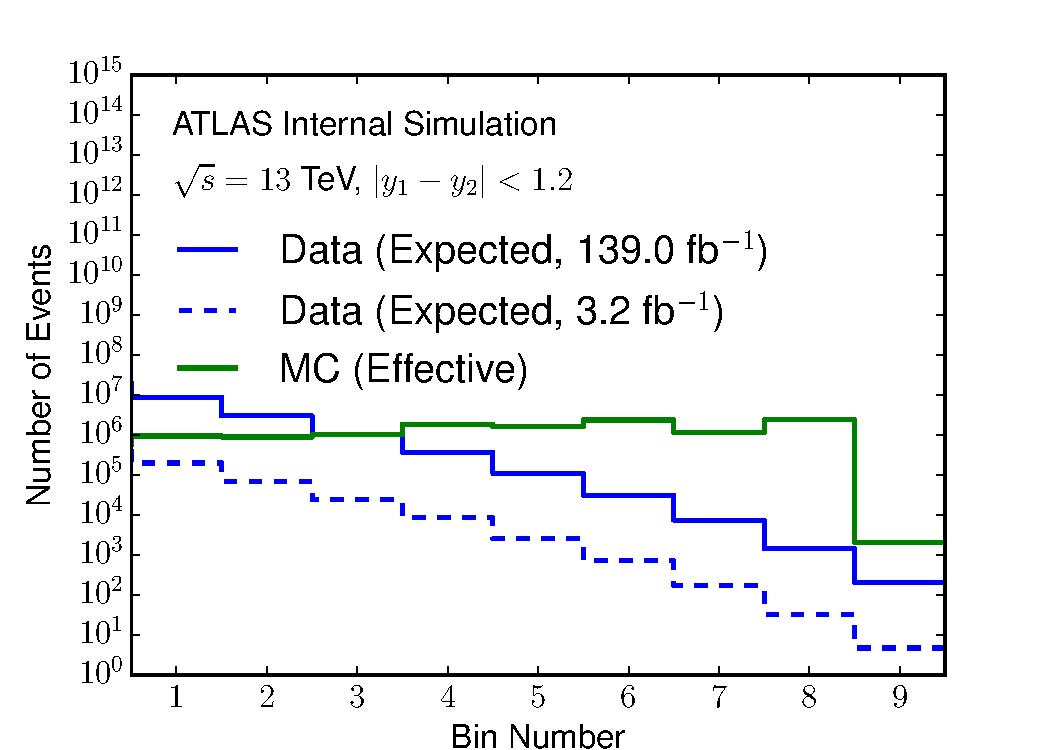
\includegraphics[width=0.45\textwidth]{figures_CWoLa/MCstats_4_10_19.pdf}}
\subfloat[]{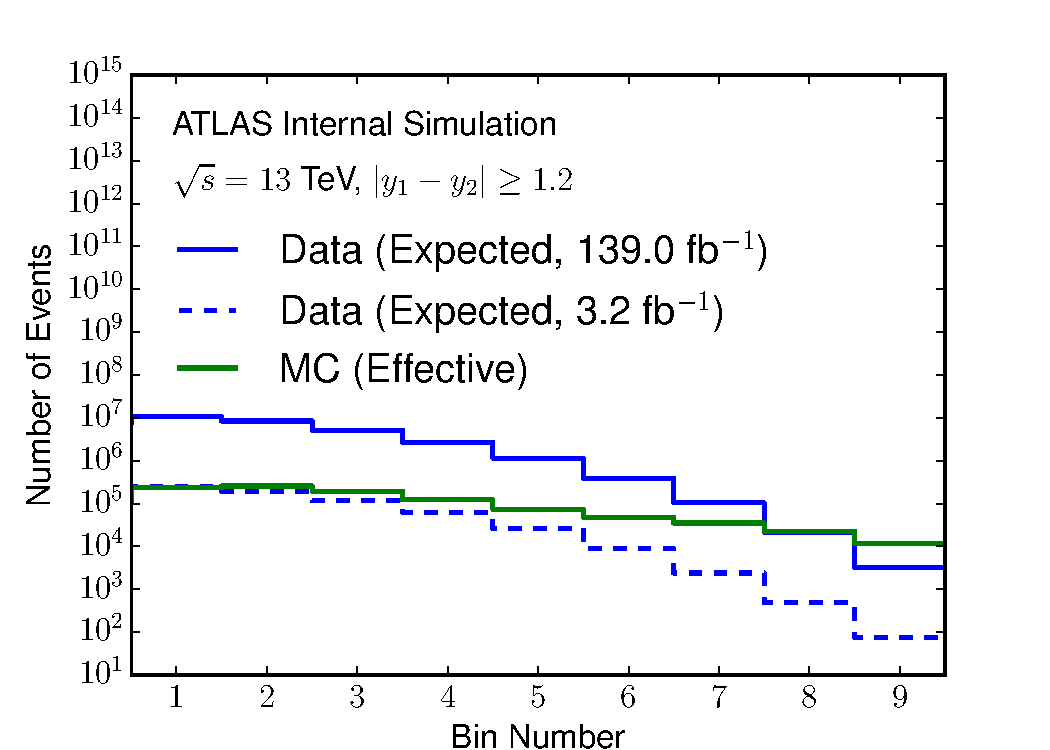
\includegraphics[width=0.45\textwidth]{figures_CWoLa/MCstats_yinvert_4_10_19.pdf}}
\caption{The effective statistics for the nominal rapidity difference (a) and the inverted one (b) for MC and data and for different integrated luminosities.}
\label{fig:CWoLa:effectivestats}
\end{figure}

The inverted dataset has about ten times more events than the nominal rapidity difference dataset above about 3 TeV, which can be seen in Figure~\ref{fig:CWoLa:invertedcutratio}.
In order for the inverted dataset to have comparable statistics to the nominal dataset for testing our methodology, random sampling without replacement is used to reduce the dataset.
The random sampling rate is determined from a fit to the ratio of efficiencies for the two rapidity differences cuts (also shown in Figure~\ref{fig:CWoLa:invertedcutratio})
\footnote{In principle, by looking at this distribution, we have unblinded the full dataset with no NN cut.  However, we have not examined this distribution in detail and have not performed any statistical tests on the quality of the fit.  It actually may be easier to do the bump hunt in this ratio, which is relatively flat, but this is left for future studies.}.

\begin{figure}[h!]
\centering
\includegraphics[width=0.45\textwidth]{figures_CWoLa/{yinvert_eff_fit_11.2.19}.pdf}
\caption{The ratio of efficiencies for the two rapidity differences cuts.  A fit shown with a dashed line is the sum of two power law functions.  Note that these are data plots and not simulation.}
\label{fig:CWoLa:invertedcutratio}
\end{figure}

As will be mentioned in Section~\ref{sec:CWoLa:fitting}, each analysis imposes a cut of $m_{JJ}>1.8$ TeV for the fitting.
For the simulation analysis, as mentioned above, the effective MC statistics are only reliable above around that value.
For the data analyses, this cut results mainly from the finding that the fitting procedure simply is not sufficient to describe the background shape for the high numbers of events seen below that cut\footnote{A more sophisticated (possibly non-parametric) fitting procedure may be able to extend the search to lower values in the future.}.
However, it is also the case that the inverted rapidity selection provides multiple copies of independent datasets to test the analysis when the ratio of efficiencies is $<\frac{1}{2}$;
in particular, the ratio of efficiencies is $<\frac{1}{3}$ (so $3$ statistically independent copies) for $m_{JJ}>\sim 1.8$ TeV, which was useful for testing the statistical properties of the fitting.

\FloatBarrier
\section{Analysis Details}
\label{sec:CWoLa:analysis_details}

\subsection{Event Selection}
\label{sec:CWoLa:eventselection}
%The following can be considered an explication of the event selection mentioned in Analysis Step~\ref{step1}.

As mentioned in Section~\ref{sec:CWoLa:data}, data are collected using the lowest available unprescaled single-jet trigger.

%For both data and simulation, the EXOT3 derivation is used, which requires at least two \\ \texttt{AntiKt10LCTopoTrimmedPtFrac5SmallR20} jets with $\pt>100$ GeV, $|\eta|<2.8$, and (uncalibrated) $m>30$ GeV if the jet $\pt$ is less than 1000 GeV.

This analysis uses anti-$k_t$, $R=1.0$ jets reconstructed from topoclusters with the local cluster weighting scheme (LCW)~\cite{Aad:2016upy}.
The jets are trimmed~\cite{Krohn:2009th} using using the parameters $f_\text{cut} = 5\%$ and $R_\text{sub} = 0.2$.
A Monte Carlo-based particle-level calibration is then applied to the jets used in this analysis~\cite{Aaboud:2018kfi}.
It corrects on average the reconstructed mass and $p_T$ of the jets to their particle-level values.
The \textit{combined mass} measurement is used, which combines measurements from the tracking system and the calorimeter; including this information has been shown to have better mass resolution, especially at high jet $\pt$~\cite{ATLAS-CONF-2016-035}.

The offline selection that is made on top of the selection from the derivation is intended to be as fully inclusive as possible to prospective signal models, while remaining on the plateau of the turn-on for the trigger.

Each event is required to have at least two large-$R$ jets with calibrated $\pt>200$ GeV
\footnote{Jet calibrations for large-radius jets are only derived for $\pt>200$ GeV.
%In any case, the number of jets with $\pt$ between 100 and 200 GeV is negligible: 0.1\% for $m_{JJ} > 1.8$ TeV.
%The simulation and validation analyses do not remove these as they are already done and nothing noticeable will change by removing them (at the expense of a lot of additional work).  They are removed for the unblinded nominal data analysis.
}
and $|\eta|<2.0$, and with at least one such jet with calibrated $\pt>500$ GeV.
This offline threshold has been shown to be fully efficient with respect to the trigger selection~\cite{Adorni:2647394}.
There is no explicit lepton overlap removal or veto.

Only the two jets with highest $\pt$ in the event are used in this analysis, and the remaining jets are ignored.
For each jet $j=1,2$, the four-momentum $p^\mu_j$ is recorded, in particular the jet mass $m_j^2 = (p^\mu_j)^2$.
As mentioned in Section~\ref{sec:CWoLa:blinding}, a selection is placed on the rapidity difference, $|y_1-y_2|<1.2$.
%The distribution of the rapidity difference in the background simulation can be seen in Figure~\ref{fig:CWoLa:bkg_rapdiff}, and the distributions in various signal models can be seen in Figure~\ref{fig:CWoLa:sig_rapdiff}.

The jets are ordered by their mass, so that $m_1 \ge m_2$.
In order to suppress background and therefore increase sensitivity to massive signal objects, a minimum cut $m_1$, $m_2 > 30$ \GeV{} is applied
\footnote{In addition, jet calibrations for large-radius jets are only derived for $m>30$ GeV.}
.
Also, in order to make the kinematic region in which the learning is applied definite, a maximum selection $m_1$, $m_2 < 500$ \GeV{} is applied.
The reasoning behind this selection is explained in more detail in Section~\ref{sec:CWoLa:features}.

Typically the dijet invariant mass $m_{JJ}$ would be defined as in terms of the sum of the four-momenta of the two jets, $m_{JJ}^2 = (p^\mu_1+p^\mu_2)^2 = m_1^2+m_2^2+2\left(E_1E_2-\vec{p}_1\cdot\vec{p}_2\right)$, with $E^2 = |\vec{p}|^2+m^2$ and $|\vec{p}| = p_T\cosh(\eta)$.
In this analysis the dijet invariant mass is defined slightly differently: in order to reduce correlations between the features used in the neural network ($m_1,m_2$) and the final $m_{JJ}$ value, the dijet invariant mass is formed by setting all $m_i$ to zero: $m_{JJ}^2 \equiv 2\left(|\vec{p}_1||\vec{p_2}|-\vec{p}_1\cdot\vec{p}_2\right)$.
This new definition removes all correlations between $m_{JJ}$ and $m_1,m_2$ except for those arising from indirect correlations between the jet $m$ and the jet $p_T$ and $\eta$.
In practice this is a very small change, because the jets in this analysis typically have energies much larger than their masses, and so the new definition gives almost the same value for the invariant mass.
As will be discussed in Section~\ref{sec:CWoLa:binning}, a selection is applied on the dijet invariant mass of $1.1 \le m_{JJ} < 8.17$ TeV.
As will be discussed in Section~\ref{sec:CWoLa:fitting}, effectively a selection of $1.8 \le m_{JJ}$ TeV is applied as the fitting range.

These selections are summarized in Table~\ref{tab:event_selection}.
\begin{table}[htbp]
  \begin{center}
    \caption{Jet selection. The $m_{JJ}$ selection is indicated for the $m_{JJ}$ bins (Section~\ref{sec:CWoLa:binning}) and also for the fitting range (Section~\ref{sec:CWoLa:fitting}).}
  \label{tab:event_selection}
    \begin{tabular}{c c}
      \hline
      Observable & Selection \\
      \hline
      $p_T$ & $>500$ GeV ($\ge 1$ jet), $>200$ GeV ($\ge 2$ jets) \\
      $|\eta|$ & $<2.0$ \\
      $|y_1-y_2|$ & $<1.2$ \\
      $m$ & $> 30$ GeV, $<500$ GeV \\
      $m_{JJ}$ (bins) & $\ge 1.1$ TeV, $<8.17$ TeV \\
      $m_{JJ}$ (fitting) & $\ge 1.8$ TeV \\
      \hline
    \end{tabular}
  \end{center}
\end{table}

The cutflow of these selections on the signal samples is given in Table~\ref{tab:cutflow_signal}.
\begin{table}[htbp]
  \begin{adjustwidth}{-2cm}{-2cm}
  \begin{center}
    \caption{Signal sample efficiency with selections up to and including given selection. All selections are given in Section~\ref{sec:CWoLa:eventselection}. The jet selections are summarized in Table~\ref{tab:event_selection}. The $m_{JJ}$ selection is included for the binning selection of $1.1 \le m_{JJ} < 8.17$ TeV and for the additional selection from the fitting of $1.8 \le m_{JJ}$ TeV.}
  \label{tab:cutflow_signal}
    \begin{tabular}{c c c c c c c c c}
      \hline
      $(m_A,m_B,m_C)$ [\GeV] & Derivation & Trigger & \pt & $|\eta|$ & $|y_1-y_2|$ & $m$ & $m_{JJ}$ (bins) & $m_{JJ}$ (fitting) \\
      \hline
      (3000,80,80)   & 1.00 & 0.90 & 0.85 & 0.85 & 0.64 & 0.63 & 0.62 & 0.59 \\
      (3000,80,200)  & 1.00 & 0.91 & 0.85 & 0.85 & 0.63 & 0.62 & 0.61 & 0.58 \\
      (3000,80,400)  & 1.00 & 0.92 & 0.81 & 0.81 & 0.61 & 0.60 & 0.58 & 0.56 \\
      (3000,200,200) & 1.00 & 0.93 & 0.87 & 0.87 & 0.64 & 0.63 & 0.63 & 0.59 \\
      (3000,200,400) & 1.00 & 0.95 & 0.84 & 0.84 & 0.62 & 0.61 & 0.60 & 0.58 \\
      (3000,400,400) & 1.00 & 0.95 & 0.82 & 0.82 & 0.62 & 0.60 & 0.59 & 0.57 \\
      (5000,80,80)   & 1.00 & 0.68 & 0.58 & 0.58 & 0.44 & 0.44 & 0.42 & 0.34 \\
      (5000,80,200)  & 1.00 & 0.70 & 0.59 & 0.59 & 0.45 & 0.44 & 0.42 & 0.34 \\
      (5000,80,400)  & 1.00 & 0.78 & 0.58 & 0.58 & 0.44 & 0.43 & 0.40 & 0.34 \\
      (5000,200,200) & 1.00 & 0.75 & 0.63 & 0.63 & 0.48 & 0.47 & 0.45 & 0.37 \\
      (5000,200,400) & 1.00 & 0.82 & 0.65 & 0.65 & 0.49 & 0.48 & 0.45 & 0.39 \\
      (5000,400,400) & 1.00 & 0.88 & 0.68 & 0.68 & 0.50 & 0.48 & 0.47 & 0.43 \\
      \hline
    \end{tabular}
  \end{center}
  \end{adjustwidth}
\end{table}

\FloatBarrier
\subsection{Binning}
\label{sec:CWoLa:binning}
As mentioned in Analysis Step~\ref{step2}, the $m_{JJ}$ spectrum is binned in order to derive the signal and sideband regions.
The size of the binning is chosen to be 20\%, guided by the dijet mass resolution of the signal models.
The minimum $m_{JJ}$ value is 1.1 TeV, due to the jet and trigger selection, and the maximum value is at 8.17 TeV (the right edge of bin $10$ with 20\% bin size), above which few events are expected to be observed.
Since every event is required to lie in an $m_{JJ}$ bin, effectively an event selection is therefore applied for $1.1 \le m_{JJ} < 8.17$ TeV.
The bin definitions are given in Table~\ref{tab:mjj_bins}.

\begin{table}[htb]
  \centering
  \caption{\label{tab:mjj_bins} $m_{JJ}$ bin definitions.}
  \begin{tabular}{c c}
    \hline
    Bin & Definition  \\ \hline
    0 & $1.10 \le m_{JJ} < 1.32$ TeV \\
    1 & $1.32 \le m_{JJ} < 1.58$ TeV \\
    2 & $1.58 \le m_{JJ} < 1.90$ TeV \\
    3 & $1.90 \le m_{JJ} < 2.28$ TeV \\
    4 & $2.28 \le m_{JJ} < 2.74$ TeV \\
    5 & $2.74 \le m_{JJ} < 3.28$ TeV \\
    6 & $3.28 \le m_{JJ} < 3.94$ TeV \\
    7 & $3.94 \le m_{JJ} < 4.73$ TeV \\
    8 & $4.73 \le m_{JJ} < 5.68$ TeV \\
    9 & $5.68 \le m_{JJ} < 6.81$ TeV \\
    10 & $6.81 \le m_{JJ} < 8.17$ TeV \\
    \hline
  \end{tabular}
\end{table}

The distribution of $m_{JJ}$ in the background with these bin definitions is shown in Figure~\ref{fig:CWoLa:bkg_mjj}.
It can be seen that the distribution of $m_{JJ}$ in the background before any cuts is smooth, with no bumps indicating possible discoveries.
\begin{figure}[htbp]
  \centering 
  \subfloat[]{\includegraphics[width=0.6\textwidth]{figures_CWoLa/{mjj_loglog_4.10.19}.pdf}}
  \caption{Distribution of $m_{JJ}$ in the background MC. The green lines indicate the bin edges of $m_{JJ}$ regions 0-10.}
\label{fig:CWoLa:bkg_mjj}
\end{figure}

The distributions of $m_{JJ}$ in a variety of signal models are shown in Figure~\ref{fig:CWoLa:sig_mjj}.
It can be seen that the mass of the signal object, $m_A$, is well-reconstructed as $m_{JJ}$, with significant tails at lower $m_{JJ}$ values.
The resolution of $m_A$ with $m_{JJ}$ is roughly 20\%, which guides the sizing of the binning, as mentioned above.

\begin{figure}[htbp]
  \centering 
  \subfloat[]{\includegraphics[width=0.3\textwidth]{figures_CWoLa/{mjj_loglog_vlines_Wprime_WZqqqq_M3000_m80_m80_1.14.20}.pdf}}
  \subfloat[]{\includegraphics[width=0.3\textwidth]{figures_CWoLa/{mjj_loglog_vlines_Wprime_WZqqqq_M3000_m80_m200_1.14.20}.pdf}}
  \subfloat[]{\includegraphics[width=0.3\textwidth]{figures_CWoLa/{mjj_loglog_vlines_Wprime_WZqqqq_M3000_m80_m400_1.14.20}.pdf}}\\
  \subfloat[]{\includegraphics[width=0.3\textwidth]{figures_CWoLa/{mjj_loglog_vlines_Wprime_WZqqqq_M3000_m200_m200_1.14.20}.pdf}}
  \subfloat[]{\includegraphics[width=0.3\textwidth]{figures_CWoLa/{mjj_loglog_vlines_Wprime_WZqqqq_M3000_m200_m400_1.14.20}.pdf}}
  \subfloat[]{\includegraphics[width=0.3\textwidth]{figures_CWoLa/{mjj_loglog_vlines_Wprime_WZqqqq_M3000_m400_m400_1.14.20}.pdf}}\\
  \subfloat[]{\includegraphics[width=0.3\textwidth]{figures_CWoLa/{mjj_loglog_vlines_Wprime_WZqqqq_M5000_m80_m80_1.14.20}.pdf}}
  \subfloat[]{\includegraphics[width=0.3\textwidth]{figures_CWoLa/{mjj_loglog_vlines_Wprime_WZqqqq_M5000_m80_m200_1.14.20}.pdf}}
  \subfloat[]{\includegraphics[width=0.3\textwidth]{figures_CWoLa/{mjj_loglog_vlines_Wprime_WZqqqq_M5000_m80_m400_1.14.20}.pdf}}\\
  \subfloat[]{\includegraphics[width=0.3\textwidth]{figures_CWoLa/{mjj_loglog_vlines_Wprime_WZqqqq_M5000_m200_m200_1.14.20}.pdf}}
  \subfloat[]{\includegraphics[width=0.3\textwidth]{figures_CWoLa/{mjj_loglog_vlines_Wprime_WZqqqq_M5000_m200_m400_1.14.20}.pdf}}
  \subfloat[]{\includegraphics[width=0.3\textwidth]{figures_CWoLa/{mjj_loglog_vlines_Wprime_WZqqqq_M5000_m400_m400_1.14.20}.pdf}}\\
  \caption{Distribution of $m_{JJ}$ for a signal model with:\\
    (a) ($m_A,m_B,m_C=3000,80,80$ GeV);
    (b) ($m_A,m_B,m_C=3000,200,80$ GeV);\\
    (c) ($m_A,m_B,m_C=3000,400,80$ GeV);
    (d) ($m_A,m_B,m_C=3000,200,200$ GeV);\\
    (e) ($m_A,m_B,m_C=3000,400,20$ GeV);
    (f) ($m_A,m_B,m_C=3000,400,400$ GeV);\\
    (g) ($m_A,m_B,m_C=5000,80,80$ GeV);
    (h) ($m_A,m_B,m_C=5000,200,80$ GeV);\\
    (i) ($m_A,m_B,m_C=5000,400,80$ GeV);
    (j) ($m_A,m_B,m_C=5000,200,200$ GeV);\\
    (k) ($m_A,m_B,m_C=5000,400,20$ GeV);
    (l) ($m_A,m_B,m_C=5000,400,400$ GeV).
  }
\label{fig:CWoLa:sig_mjj}
\end{figure}

One thing to note about this analysis is that the binning is fixed.
A possible issue with this is that for a signal that is found close to the edge of a bin, the NN may not learn to tag that signal because it has presence in both that bin and its sideband.
This effect is mitigated somewhat due to two factors: (1) Because the background is steeply falling, there is only a small region of $m_A$ in which the signal fraction in both a signal bin and its sideband are comparable; and (2) the NN is trained on both sidebands simultaneously, so that the signal should still be tagged when distinguishing between the signal region and the combined sidebands even if it lies on the edge.
A study of this effect is presented in Appendix~\ref{app:CWoLa:binoffset}.

\FloatBarrier
\subsection{Features}
\label{sec:CWoLa:features}
In Analysis Step~\ref{step4}, some features $X$ are designated which, as per Assumption~\ref{ass1}, can be used to distinguish signals from the background.
In this analysis, only the masses of the two jets, $X = \{m_1,m_2\}$, are used as features.

The distributions of $m_1$ and $m_2$ in the background using the nominal simulation are plotted in various $m_{JJ}$ regions in Figure~\ref{fig:CWoLa:bkg_m1_m2}.
The distributions of $m_1$ and $m_2$ in a variety of signal models are plotted in the $m_{JJ}$ region which is most efficient on that signal in Figure~\ref{fig:CWoLa:sig_m1_m2}.
It can be seen that the masses of the signal objects, $m_B$ and $m_C$, are well-reconstructed as $m_1$ and $m_2$.

\begin{figure}[htbp]
  \centering 
  \subfloat[]{\includegraphics[width=0.3\textwidth]{figures_CWoLa/{jet1_m_jet2_m_sigR0_4.10.19}.png}}
  \subfloat[]{\includegraphics[width=0.3\textwidth]{figures_CWoLa/{jet1_m_jet2_m_sigR1_4.10.19}.png}}
  \subfloat[]{\includegraphics[width=0.3\textwidth]{figures_CWoLa/{jet1_m_jet2_m_sigR2_4.10.19}.png}}\\
  \subfloat[]{\includegraphics[width=0.3\textwidth]{figures_CWoLa/{jet1_m_jet2_m_sigR3_4.10.19}.png}}
  \subfloat[]{\includegraphics[width=0.3\textwidth]{figures_CWoLa/{jet1_m_jet2_m_sigR4_4.10.19}.png}}
  \subfloat[]{\includegraphics[width=0.3\textwidth]{figures_CWoLa/{jet1_m_jet2_m_sigR5_4.10.19}.png}}\\
  \subfloat[]{\includegraphics[width=0.3\textwidth]{figures_CWoLa/{jet1_m_jet2_m_sigR6_4.10.19}.png}}
  \subfloat[]{\includegraphics[width=0.3\textwidth]{figures_CWoLa/{jet1_m_jet2_m_sigR7_4.10.19}.png}}
  \subfloat[]{\includegraphics[width=0.3\textwidth]{figures_CWoLa/{jet1_m_jet2_m_sigR8_4.10.19}.png}}\\
  \subfloat[]{\includegraphics[width=0.3\textwidth]{figures_CWoLa/{jet1_m_jet2_m_sigR9_4.10.19}.png}}
  %\subfloat[]{\includegraphics[width=0.3\textwidth]{figures_CWoLa/{jet1_m_jet2_m_sigR10_4.10.19}.pdf}}
  \caption{Distribution of $m_1$ and $m_2$ in the background simulation in $m_{JJ}$ regions (a) 0; (b) 1; (c) 2; (d) 3; (e) 4; (f) 5; (g) 6; (h) 7; (i) 8; (j) 9.}
\label{fig:CWoLa:bkg_m1_m2}
\end{figure}

\begin{figure}[htbp]
  \centering 
  \subfloat[]{\includegraphics[width=0.3\textwidth]{figures_CWoLa/{jet1_m_jet2_m_Wprime_WZqqqq_M3000_m80_m80_1.14.20}.pdf}}
  \subfloat[]{\includegraphics[width=0.3\textwidth]{figures_CWoLa/{jet1_m_jet2_m_Wprime_WZqqqq_M3000_m80_m200_1.14.20}.pdf}}
  \subfloat[]{\includegraphics[width=0.3\textwidth]{figures_CWoLa/{jet1_m_jet2_m_Wprime_WZqqqq_M3000_m80_m400_1.14.20}.pdf}}\\
  \subfloat[]{\includegraphics[width=0.3\textwidth]{figures_CWoLa/{jet1_m_jet2_m_Wprime_WZqqqq_M3000_m200_m200_1.14.20}.pdf}}
  \subfloat[]{\includegraphics[width=0.3\textwidth]{figures_CWoLa/{jet1_m_jet2_m_Wprime_WZqqqq_M3000_m200_m400_1.14.20}.pdf}}
  \subfloat[]{\includegraphics[width=0.3\textwidth]{figures_CWoLa/{jet1_m_jet2_m_Wprime_WZqqqq_M3000_m400_m400_1.14.20}.pdf}}\\
  \subfloat[]{\includegraphics[width=0.3\textwidth]{figures_CWoLa/{jet1_m_jet2_m_Wprime_WZqqqq_M5000_m80_m80_1.14.20}.pdf}}
  \subfloat[]{\includegraphics[width=0.3\textwidth]{figures_CWoLa/{jet1_m_jet2_m_Wprime_WZqqqq_M5000_m80_m200_1.14.20}.pdf}}
  \subfloat[]{\includegraphics[width=0.3\textwidth]{figures_CWoLa/{jet1_m_jet2_m_Wprime_WZqqqq_M5000_m80_m400_1.14.20}.pdf}}\\
  \subfloat[]{\includegraphics[width=0.3\textwidth]{figures_CWoLa/{jet1_m_jet2_m_Wprime_WZqqqq_M5000_m200_m200_1.14.20}.pdf}}
  \subfloat[]{\includegraphics[width=0.3\textwidth]{figures_CWoLa/{jet1_m_jet2_m_Wprime_WZqqqq_M5000_m200_m400_1.14.20}.pdf}}
  \subfloat[]{\includegraphics[width=0.3\textwidth]{figures_CWoLa/{jet1_m_jet2_m_Wprime_WZqqqq_M5000_m400_m400_1.14.20}.pdf}}\\
  \caption{Distribution of $m_1$ and $m_2$ for a signal model with:\\
    (a) ($m_A,m_B,m_C=3000,80,80$ GeV);
    (b) ($m_A,m_B,m_C=3000,200,80$ GeV);\\
    (c) ($m_A,m_B,m_C=3000,400,80$ GeV);
    (d) ($m_A,m_B,m_C=3000,200,200$ GeV);\\
    (e) ($m_A,m_B,m_C=3000,400,20$ GeV);
    (f) ($m_A,m_B,m_C=3000,400,400$ GeV);\\
    (g) ($m_A,m_B,m_C=5000,80,80$ GeV);
    (h) ($m_A,m_B,m_C=5000,200,80$ GeV);\\
    (i) ($m_A,m_B,m_C=5000,400,80$ GeV);
    (j) ($m_A,m_B,m_C=5000,200,200$ GeV);\\
    (k) ($m_A,m_B,m_C=5000,400,200$ GeV);
    (l) ($m_A,m_B,m_C=5000,400,400$ GeV).
  }
\label{fig:CWoLa:sig_m1_m2}
\end{figure}

Since $m_1$ and $m_2$ peak around the values of $m_B$ and $m_C$ in the signal, while they have smoothly falling spectra in the background, these features satisfy Assumption~\ref{ass1}, and therefore can be used for the training.

\FloatBarrier
\subsubsection{Mass Decorrelation}
\label{sec:CWoLa:decorrelation}
In Figure~\ref{fig:CWoLa:bkg_m1_m2}, it can be seen that there are true physical differences in the features in the background between a given signal region and sideband regions (as chosen in Analysis Step~\ref{step3}); in particular, the distribution gets more populated at higher $m_1$,$m_2$ as $m_{JJ}$ increases.
This therefore requires some modification of these features in order to satisfy Assumption~\ref{ass2}.

The idea is to scale the 1-dimensional marginal distribution of the jet mass $m$ (combining both $m_1$ and $m_2$ across all events) in the sideband regions to the signal region.
This is accomplished by constructing the empirical cumulative distribution function (ECDF) in each region $s$:
\begin{align}
  \Phi_s(m) = \frac{1}{n_s} \sum_{j=1}^{n_s} \mathbbm{1}(m_j\le m)
\end{align}
Where $n_s$ is the number of jets in $m_{JJ}$ region $s$, $\mathbbm{1}$ is the indicator function, and $j$ goes over all jets (leading and subleading) in region $s$.\footnote{Actually, $\Phi_s(m)$ is evaluated at all values of $m$ that exist in the $m_{JJ}$ region, and then is linearly interpolated for intermediate values.}
Note that the distribution of $\Phi_s(m)$ over all jets in $m_{JJ}$ region $s$ is by definition uniform; and that the distribution of $\Phi^{-1}_s(x)$ is exactly the distribution of $m$ in $m_{JJ}$ region $s$, if $x$ follows a uniform distribution.
The ECDF is a good approximation of the true CDF in regions where there are a sufficient number of samples.
This motivates the choice to place a maximum cut on the jet mass at $500 \GeV$, in order to restrict to the region in which the CDF can be approximated well.

Then, for a given signal segion $s$, the masses of all jets in the sideband segions $s-1$ and $s+1$ are rescaled to the signal segion:
\begin{align}
  \begin{cases}
    m \rightarrow \Phi^{-1}_s\left(\Phi_{s-1}\left(m\right)\right) & m \in \text{region } s-1 \\
    m \rightarrow \Phi^{-1}_s\left(\Phi_{s+1}\left(m\right)\right) & m \in \text{region } s+1
  \end{cases}
\end{align}
This ensures that the 1-dimensional distributions of $m$ in the sideband regions are exactly the same, by construction, as in the signal region.
Note that, if there is a signal present in the signal region, that the scaling will be slightly biased by the presence of this signal, depending on the signal fraction in that region.
This scaling is demonstrated for an example signal and sideband regions in Figure~\ref{fig:CWoLa:m_scaling}, including an example with an injected signal.
\begin{figure}[t!]
    \centering
    \subfloat[]{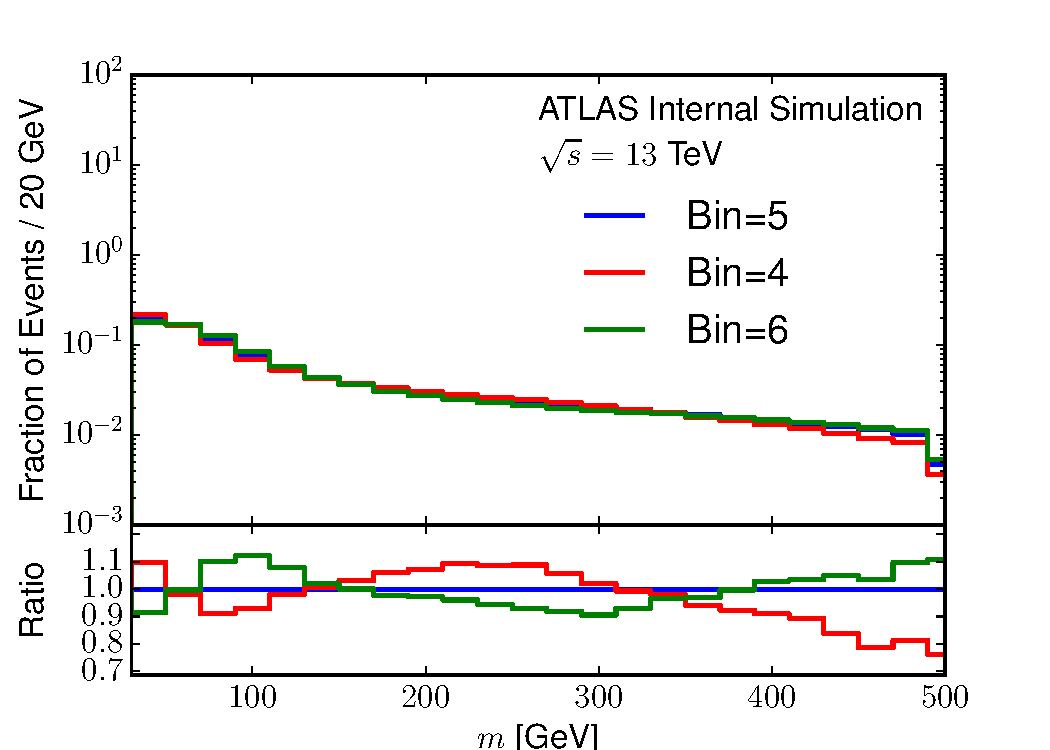
\includegraphics[width=0.45\textwidth]{{figures_CWoLa/jet_m_log_mjjbins_sigR5_4.10.19}.pdf}}
    \subfloat[]{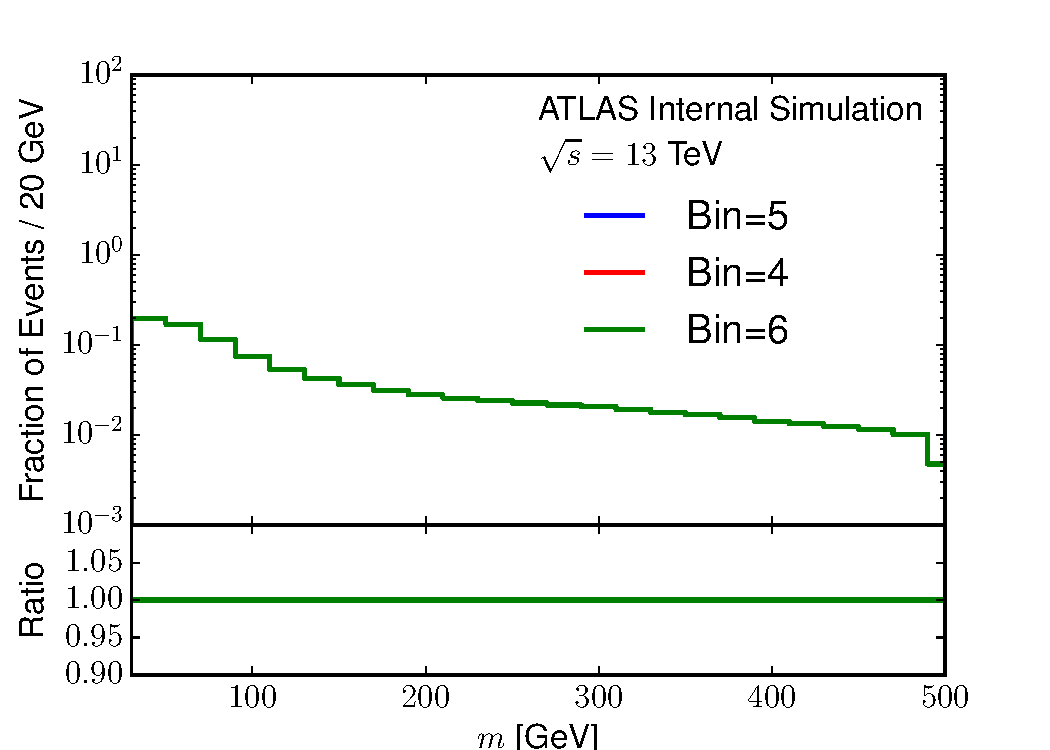
\includegraphics[width=0.45\textwidth]{{figures_CWoLa/jet_m_scaled_log_mjjbins_sigR5_4.10.19}.pdf}}\\
    \subfloat[]{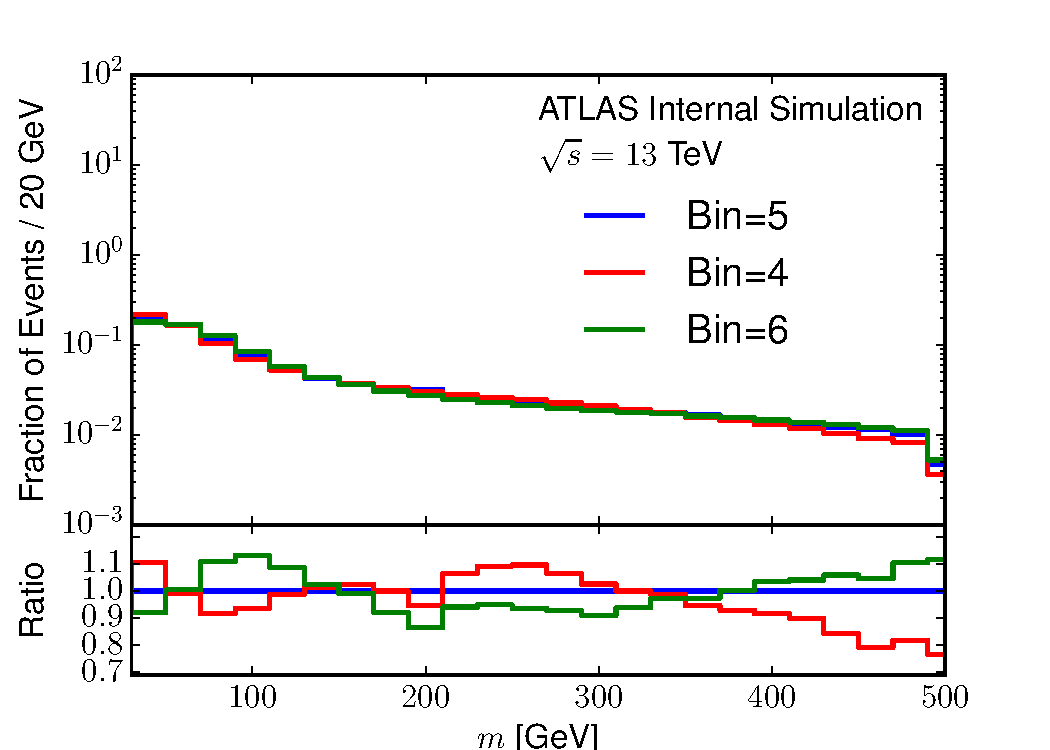
\includegraphics[width=0.45\textwidth]{{figures_CWoLa/jet_m_log_mjjbins_sigR5_Wprime_WZqqqq_M3000_m200_m200_nS2000_4.10.19}.pdf}}
    \subfloat[]{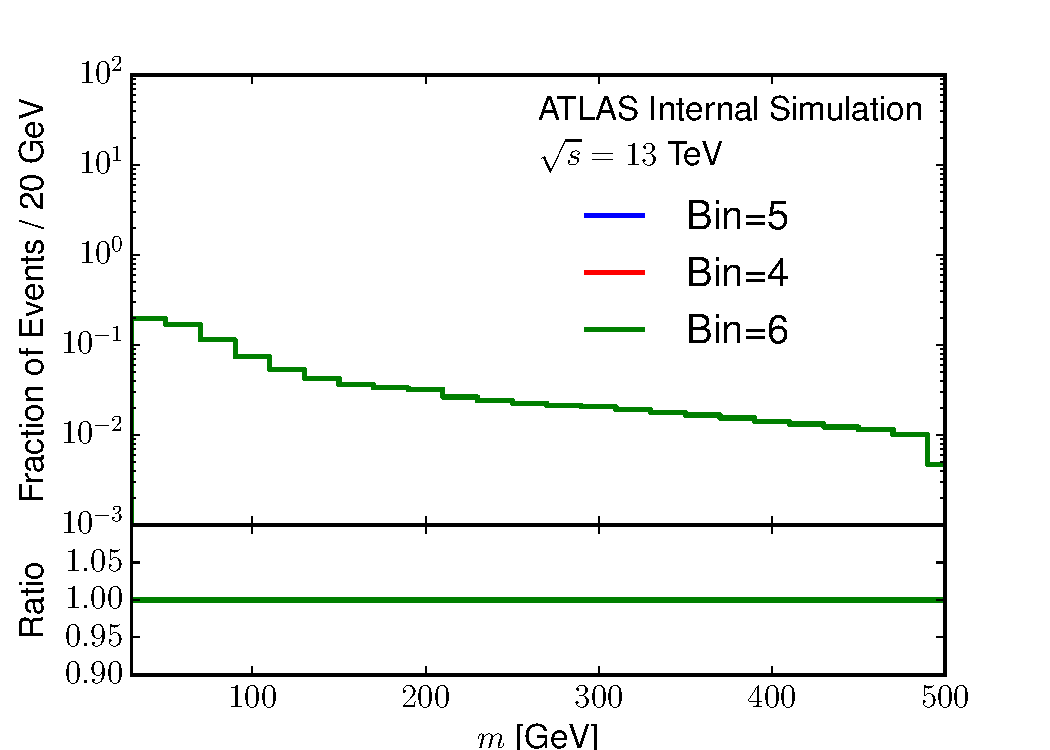
\includegraphics[width=0.45\textwidth]{{figures_CWoLa/jet_m_scaled_log_mjjbins_sigR5_Wprime_WZqqqq_M3000_m200_m200_nS2000_4.10.19}.pdf}}
    \caption{The distributions of $m$ in simulation, comparing between signal region $s=5$ and sideband regions $s-1=4$ and $s+1=6$.
    (a) Before any scaling.
    (b) After scaling via the empirical cumulative distribution function.
    (c) Including an injected signal sample with $m_A,m_B,m_C=3000,200,200$ GeV, which lies mostly in signal segion 5, and with $\frac{S}{\sqrt{B}}\sim 2$ in that region.
    (d) After scaling, with the presence of the signal sample.}
    \label{fig:CWoLa:m_scaling}
\end{figure}

After the 1-dimensional scaling the only differences that can exist are in the 2-dimensional distribution $m_1$ and $m_2$, which can arise due to differences in the correlation between $m_1$ and $m_2$ between the regions.
It is expected that in the background these differences are small, and this is supported by examining the distributions of $m_1$ and $m_2$ in simulation, as can be seen in Figure~\ref{fig:CWoLa:LR2D}.

In order to additionally remove correlations between the features and $m_{JJ}$, the left and right sidebands are combined with equal total weight for the training (Section~\ref{sec:CWoLa:network}).
Then the distribution of the features in the combined sidebands is exactly the average of the distribution in the left and right sidebands, removing first-order dependencies of the features on $m_{JJ}$.

The presence of a signal in one of the regions is exactly such a difference that can exist in the correlations between $m_1$ and $m_2$.
Therefore, even though the scaling can be biased by the presence of a signal in the signal region, it is expected that there will still exist differences in the 2-dimensional distribution between the signal and sideband regions, as can be seen in Figure~\ref{fig:CWoLa:LR2D}.
\begin{figure}[t!]
    \centering
    \subfloat[]{\includegraphics[width=0.3\textwidth]{{figures_CWoLa/jet_m1_m2_scaled_ratiolow_sigR5_scaleall_4.10.19}.pdf}}
    \subfloat[]{\includegraphics[width=0.3\textwidth]{{figures_CWoLa/jet_m1_m2_scaled_ratiohigh_sigR5_scaleall_4.10.19}.pdf}}
    \subfloat[]{\includegraphics[width=0.3\textwidth]{{figures_CWoLa/jet_m1_m2_scaled_ratio_sigR5_scaleall_4.10.19}.pdf}}\\
    \subfloat[]{\includegraphics[width=0.3\textwidth]{{figures_CWoLa/jet_m1_m2_scaled_ratiolow_sigR5_Wprime_WZqqqq_M3000_m200_m200_nS2000_4.10.19}.pdf}}
    \subfloat[]{\includegraphics[width=0.3\textwidth]{{figures_CWoLa/jet_m1_m2_scaled_ratiohigh_sigR5_Wprime_WZqqqq_M3000_m200_m200_nS2000_4.10.19}.pdf}}
    \subfloat[]{\includegraphics[width=0.3\textwidth]{{figures_CWoLa/jet_m1_m2_scaled_ratio_sigR5_Wprime_WZqqqq_M3000_m200_m200_nS2000_4.10.19}.pdf}}
    \caption{The 2-dimensional likelihood ratio in $m_1$ and $m_2$ after scaling, comparing between signal region $s=5$ and (a) sideband region $s-1=4$;
      (b) sideband region $s+1=6$;
      and (c) combining sideband regions $4$ and $6$.
      (d,e,f) Including an injected signal sample with $m_A,m_B,m_C=3000,200,200$ GeV, which lies mostly in signal region 5, and with $\frac{S}{\sqrt{B}}\sim 2$ in that region.
      N.B. This Figure may appear fuzzy if viewing in macOS Preview; using a different PDF viewer, e.g. Google Chrome, seems to fix the problem.
  }
    \label{fig:CWoLa:LR2D}
\end{figure}

\FloatBarrier

\subsection{Neural Network Architecture}
\label{sec:CWoLa:network}
The neural network which determines the final score for each event, indicating more or less signal-like, is derived in multiple stages.
Neural networks have been shown to have excellent performance on a wide variety of training tasks with limited training data~\cite{haykin1994neural,Kriesel2007NeuralNetworks,bishop_2013,reed_marks_1999,goodfellow_bengio_courville_2017,ng2000cs229}.

These stages are intended to maximize the sensitivity to new potential signals, while remaining robust to statistical fluctuations and true correlations in the background.

In Analysis Step~\ref{step3} (Section~\ref{sec:CWoLa:Analysis:Overview}), some signal bin $s$ is designated. The process below can then be considered an enumeration of the steps in Analysis Step~\ref{step4} (Section~\ref{sec:CWoLa:Analysis:Overview}).
See also Figure~\ref{fig:CWoLa:flowchart} for an overview. 

\begin{enumerate}
  \item Designate the sideband regions $s+1$ (the ``upper" sideband) and $s-1$ (the ``lower" sideband). 
  \label{NNstep2}
  \item All events in the entire dataset are separated randomly into 5 equally-sized \textit{cross-validation} sets $i \in [0-4]$.
  \label{NNstep1}
  \item Designate one of the cross-validation sets $i_t$ as the \textit{test set}.
  \label{NNstep3}
  \item Designate a different cross-validation set $i_v \ne i_t$ as the \textit{validation set}. The remaining 3 cross-validation sets are designated as the \textit{training set}.
  \label{NNstep5}
  \item A neural network is trained using only the training set, with features $X = \{m_1,m_2\}$, rescaled as described in Section~\ref{sec:CWoLa:decorrelation}. The events are labeled with $Y \in [0,1]$, with $1$ indicating an event in the signal region, and $0$ indicating an event in the sidebands. The events in each of the sideband regions are weighted uniformly in the training so that the sum of weights in each of the sideband regions is equal.

  The network is a Sequential Neural Network with 4 hidden layers of size 64,32,8,1, and activation functions \texttt{ReLu},\texttt{ReLu},\texttt{ReLu},sigmoid, respectively, as implemented in \texttt{Keras}~\cite{chollet2015keras}.
  The loss used is the binary cross-entropy, and the training loss is minimized using the \texttt{Adam}~\cite{kingma2014adam} optimizer.
  The loss is evaluated on the validation set.
  
  Total number of epochs is 1000, with an early stopping with patience of 100 on the validation loss. The batch size is 1\% of the total.

  
  \label{NNstep6}
  \item Repeat Step~\ref{NNstep6} with 3 different random initial configurations of the neural network weights, and choose the network with the lowest validation loss. The other 2 networks are discarded.
  \label{NNstep7}

  Finally, this network is evaluated on the test set, and only the scores on the test set are recorded.

  \textbf{Scaling}
  \phantomsection
  \label{NNstep7scaling}

  The score from the neural network output is scaled monotonically as a quantile between 0 and 1 on the events in the signal region test set (note that the scores for all events in the test set are recorded, not just those in the signal region).
  That is to say, after the scaling, an event with a score of $0 \le \epsilon \le 1$ received a higher score from the neural network than exactly a fraction $\epsilon$ of the events in the signal region test set.
  The scaling is done in this way so that different networks can later be combined by averaging their scores; since the network output score is standardized, this averaging is meaningful.
  \item Repeat Steps~\ref{NNstep5}-\ref{NNstep7} by varying $i_v$ to each of the remaining cross-validation sets in turn, keeping the test set $i_t$ fixed.
    I.e., there are 4 different validation set choices for the given test set, and these steps are repeated for each one, resulting in 4 different networks.
    The scores from these 4 networks are then averaged, and the average score is further rescaled as described in Step~\ref{NNstep7scaling}.
  \label{NNstep8}
  \item Repeat Steps~\ref{NNstep3}-\ref{NNstep8} by varying the chosen test set $i_t$, for a total of 5 networks.
  The total sample is then combined together; since the score from each network is scaled to be an efficiency on its respective test set, and the test sets are equally sized, the score for each event remains an efficiency over the entire dataset.
  \label{NNstep9}
\end{enumerate}

Ultimately, there are $3\times4\times5 = 60$ neural networks trained for each signal region $s$. A flowchart of the process described above is given in Figure~\ref{fig:CWoLa:flowchart}, and the neural network outputs are shown at each step in the process for a sample with injected signal.

The events are separated into training, validation, and test sets as described above in order to reduce the effect of statistical fluctuations in the training.
Since the validation set is statistically independent from the training set, choosing the network with the lowest validation loss, as described in Step~\ref{NNstep7}, ensures that the network which learns true correlations the best is chosen.
Since the test set is statistically independent from both the training and validation sets, the network cannot do artificially better by being biased by statistical fluctuations in the training or validation set.
This is actually a crucially important point for removing the look-elsewhere effect in this analysis.
If the network were trained and tested on the same dataset, one would expect a high rate of false positives in terms of being able to separate the signal region from the sidebands due to correlated (actually, the same) statistical fluctuations between the train and test sets, which results directly in a bump in the $m_{JJ}$ spectrum.
Because the train and validation sets are statistically independent from the test set, the statistical fluctuations are uncorrelated, and in the case that there is no true signal the rate of false positives is no more than that expected due to a random classifier. 

The choice to train 4 different networks with each non-test set chosen to be a validation set in succession, as described in Step~\ref{NNstep8}, is again intended to reduce the sensitivity to statistical fluctuations in the training sets, since for each validation set the training set is (somewhat, but not entirely) different.
The averaging over the validation sets can be seen when going from the first column of Figure~\ref{fig:CWoLa:flowchart} to the second column.
%This can be seen, for example, when going from the first column of Figure~\ref{fig:CWoLa:flowchart} to the second column; the outputs for each individual validation set in the first column have clear differences from each other due to statistical fluctuations in the training sets, but after averaging the network outputs look almost identical between different test sets.

%The choice to train separate networks for the 2 sidebands, as described in Step~\ref{NNstep9}, is motivated by the desire to find features that are present in the signal region only and not in either of the sidebands, as would be expected for a true signal peak.
%If there are true correlations between $m_{JJ}$ and the features in the background, this correlation is expected to be the same when going from the lower sideband region to the signal region as from the signal region to the upper sideband region; and so averaging the networks trained between the 2 sidebands is intended to cancel out these effects.
%In Figure~\ref{fig:CWoLa:flowchart}, the networks for the upper and lower sideband (in the second column) can clearly be seen to be different, since there are true correlations in the background when comparing the signal region to either sideband.
%Each network does pick out the kinematic region near the true signal (near $m_B,m_C=200,80$ GeV) as a signal-like region, but other parts of the kinematic space also have high scores.
%Importantly, other than near the true signal, the network scores between the two sidebands are near opposites of each other, which supports the claim that the correlations are the same when going from the lower sideband to the signal region as from the signal region to the upper sideband.
%After averaging (in the third column), the kinematic region that receives the highest scores is clearly near the true signal, successfully canceling out the correlations between the two sidebands.

Note that, because of the fact that the networks between different test sets never interact, as described in Step~\ref{NNstep9}, two events with exactly the same features could in principle have different scores, if they happened to lie in different test sets.
However, because of the extensive measures taken to reduce the sensitivity to statistical fluctuations in the training set, it is expected that the final 5 networks should mostly be the same; this can be seen for example in the penultimate column of Figure~\ref{fig:CWoLa:flowchart}.

\begin{figure}[t!]
    \centering
    \includegraphics[width=0.9\textwidth]{figures_CWoLa/split_flowchart.pdf}
    \caption{Flowchart of steps in derivation of final network scores, as described in Section~\ref{sec:CWoLa:network}. The networks in the left-most column have already been chosen to have the lowest validation loss, as described in Step~\ref{NNstep7}. The networks are represented by a 2D plot showing the neural network output in the $m_1$,$m_2$ plane, as expressed as an efficiency on events, as described in Step~\ref{NNstep7scaling}. In this particular example, a signal was injected at $m_B=200$ GeV, $m_C=200$ GeV.  All plots in this figure use simulation.  Note that the amount of effective data in the left parts of the plot is actually $1/5$ of the total.}
    \label{fig:CWoLa:flowchart}
\end{figure}

%Briefly about the trials factor in $(m_1,m_2)$: no event is selected with a classifier that was trained using that event.  The nested cross-validation is like dividing the dataset in half, training on one half and testing on the other.  The nested cross-validation extends this to use $(k-1)/k$ events for training each network (all $k$-folds get a different network) and use all events for testing. 

Details about the software used to execute the analysis pipeline up to this point (Sections~\ref{sec:CWoLa:eventselection},~\ref{sec:CWoLa:binning},~\ref{sec:CWoLa:features},~\ref{sec:CWoLa:network}) can be found in Appendix~\ref{app:CWoLa:software}.

\FloatBarrier
\subsection{Systematic Uncertainties}
\label{sec:CWoLa:systs}

As will be described in Section~\ref{sec:CWoLa:fitting}, the background is estimated in a fully data-driven manner, and the only uncertainties are associated with the background fit.
The uncertainties related to the signal simulation are only relevant for setting cross-section limits (Section~\ref{sec:CWoLa:limits}).
For the signal, there are uncertainties on the jet mass scale and resolution as well as on the modeling of jet fragmentation; there is also an overall luminosity uncertainty.

The former set of uncertainties use the prescriptions of the Jet/MET group~\cite{TWiki_JetUncertainties_2019}.

The luminosity uncertainty for the full Run 2 dataset is 1.7\%~\cite{TWiki_LuminosityUncertainty}.
It is derived from the calibration of the luminosity scale using $x$-$y$ beam-separation scans, following a methodology similar to that detailed in Ref.~\cite{Aaboud:2016hhf}, and using the LUCID-2 detector for the baseline luminosity measurements \cite{LUCID2}.
The total integrated luminosity is $139$~fb$^{-1}$.

%More details are provided below.

The NN is not retrained for every systematic variation.
Instead, the NN trained with the nominal signal and then applied to the events with the kinematic properties of the jets varied according to the uncertainty.
In principle this is a conservative treatment of the uncertainties, since the NN learns what the actual signal looks like and tags the kinematic space accordingly;
training the network on the nominal signal and then applying to the varied kinematic properties can therefore lead to artificially low NN signal tagging efficiencies.
In practice, though, the uncertainties are small enough such that the total efficiency on the signal for some fixed NN selection is about the same in the nominal and varied samples.

%\subsubsection{Jet Kinematic Properties}
%The in situ uncertainty on the jet $p_\text{T}$ and jet mass are determined from momentum balancing and calorimeter-track matching, respectively~\cite{Aaboud:2018kfi}.
%Since the results from this analysis are not intended to be combined with other analyses\footnote{Any targeted analysis should be better in their sensitive parameter space, so combining would not improve the results.}, we use the Global Reduction set of nuisance parameters.
%This includes 6 jet mass scale uncertainties, 12 jet energy scale uncertainties, and one jet mass resolution uncertainty.
%The usual jet mass resolution prescription is to inflate the resolution by 20\% and symmetrize, which is accomplished with the standard tool by providing maps of smearing factors for particular topologies.
%However, since we have access to the true jet masses, and no single topology fits our signals, we use forward-folding to inflate and deflate the resolution by 20\% on a per-jet basis. 

\subsection{Fitting}
\label{sec:CWoLa:fitting}
After the application of the NN selection, a standard parametric background fit is performed to estimate the background contribution in the signal region.
As mentioned in Section~\ref{sec:CWoLa:blinding}, the fitting procedure is relatively simple for the simulation analysis, but more complex for the data validation and full unblinded analyses.
There are in addition some small differences in the fitting procedure between these latter two analyses.
Because of this, the fitting procedure for each of these analyses is broken out into separate subsections.

Details about the software used for the fitting are given in Appendix~\ref{app:CWoLa:fitting_software}.

\subsubsection{Simulation Analysis}
\label{sec:CWoLa:fitting:simulation_analysis}
The parametric fit is performed using 100 GeV bins
%actually from 2 TeV
from 1.8 TeV to 8.2 TeV\footnote{The 8.2 TeV maximum bin edge contains the 8.17 TeV maximum $m_{JJ}$ from the event selection (Section~\ref{sec:CWoLa:eventselection}); this value is essentially arbitrary as there are expected to be $<1$ events at that high $m_{JJ}$.}.
These bins are finer than the bins used for learning as described in Section~\ref{sec:CWoLa:binning}
\footnote{In the corresponding Section (~\ref{sec:CWoLa:simulation_analysis}), some example fits are shown using the $m_{JJ}$ bins themselves for the parametric fit; these are not actually used for the final results.}.

The selected fit function is the same as the one used by the all-hadronic diboson resonance search~\cite{Aad:2019fbh}:

\begin{align}
\label{eqn:CWoLa:fitfunction}
\frac{dn}{dx}=p_1(1-x)^{p_2-\xi p_3}x^{-p_3},
\end{align}

\noindent where $x=m_{JJ}/\sqrt{s}$, $p_1$ is a normalization parameter, $p_2$ and $p_3$ are dimensionless shape parameters, and $\xi=4.2955$ is a constant (this value chosen by the all-hadronic resonance search to remove correlations between $p_2$ and $p_3$).
%For simplicity, we set $\xi=0$ (in the diboson search, it is chosen to reduce correlations between $p_2$ and $p_3$).

The parameter $p_2$ is initialized to 10 and restricted to the range $[-100,100]$ and the parameter $p_3$ is initialized to $-30$ and restricted to the range $[-100,100]$ as well.
The signal region is not masked during this fit.
After the fit, the prediction is normalized to have the same integral as the data over the entire range.
As there are two free parameters, the fit produces a $2\times 2$ covariance matrix.  

The background fit is decoupled from the signal strength scan; the signal strength is used as a POI to set limits, as discussed in Section~\ref{sec:CWoLa:limits}.
A background prediction is generated as a histogram from the central values of the background fit.
There is one nuisance parameter for the background fit systematic uncertainty.
The ``up'' and ``down'' variations are created by taking the sum in quadrature of the uncertainties from the two parameters from the original background fit ($p_2$ and $p_3$).
This nuisance parameter can be profiled in the second fit used to fit the POI.   

\subsubsection{Validation Analysis}
\label{sec:CWoLa:fitting:val_analysis}
As in the fitting for the simulation analysis (Section~\ref{sec:CWoLa:fitting:simulation_analysis}), the parametric fit uses bins of size 100 GeV, spanning 1.8 TeV to 8.2 TeV.
Unlike in that fit, \textbf{the signal region is masked for this fit}.
In order to remove the dependence of a potential signal, the masked region for each bin is enlarged to include half of both the left and right neighboring bins.
In particular, the bins used for training and the windows used for masking in the fit are presented in Table~\ref{tab:mjj_bins2}.

\begin{table}[htb]
  \centering
  \caption{\label{tab:mjj_bins2} $m_{JJ}$ bin definitions and the mask regions for the background fit.}
  \begin{tabular}{c c c}
    \hline
    Bin & Definition & Mask  \\ \hline
    5 & $2.74 \le m_{JJ} < 3.28$ TeV & $2.5 \le m_{JJ} < 3.6$ TeV \\
    6 & $3.28 \le m_{JJ} < 3.94$ TeV & $3.0 \le m_{JJ} < 4.3$ TeV \\
    7 & $3.94 \le m_{JJ} < 4.73$ TeV & $3.6 \le m_{JJ} < 5.2$ TeV \\
    8 & $4.73 \le m_{JJ} < 5.68$ TeV & $4.3 \le m_{JJ} < 6.2$ TeV \\
    9 & $5.68 \le m_{JJ} < 6.81$ TeV & $5.2 \le m_{JJ} < 7.5$ TeV \\
    \hline
  \end{tabular}
\end{table} 

The fitting procedure then proceeds as follows:

\begin{enumerate}
  \item \label{fitstep:1} Perform a fit using the sidebands using Equation~\ref{eqn:CWoLa:fitfunction}.  Compute the $\chi^2$ in the sideband:

\begin{align}
%\chi^2=\sum_{i=1}^N \frac{(\text{data in bin $i$}-\text{fit in bin $i$})^2}{\text{fit in bin $i$}},
\chi^2=\sum_{i=1}^N \frac{(O_i-E_i)^2}{E_i},
\end{align}

\noindent where $O_i$ is the number of events observed in data in bin $i$, $E_i$ is the expected number of events from the fit function in bin $i$, and the sum runs over all $N$ sideband bins.
The parameter $p_1$ is fixed by the normalization in the sidebands.
The sideband $p$-value is then computed using $N-3$ degrees of freedom, since there are 3 fit parameters.
If this $p$-value is greater than $0.05$, move on to step~\ref{fitstep:4}, else:
\item \label{fitstep:2} Try an extended fit function:

\begin{align}
\frac{dn}{dx}=p_1(1-x)^{p_2-\xi_1 p_3}x^{-p_3+(p_4-\xi_2p_3-\xi_3p_2)\log(x)}.
\end{align}

\noindent As before, compute the sideband $p$-value (now with $N-4$ degrees of freedom).
If this $p$-value is greater than $0.05$, move on to step~\ref{fitstep:4}, else:

\item \label{fitstep:3} Try with the UA2 fit function~\cite{Alitti:1990kw}:

\begin{align}
\frac{dn}{dx}=p_1x^{p_2-\xi_1 p_3}e^{-p_3x+(p_4-\xi_2p_3-\xi_3p_2)x^2}.
\end{align}

\noindent As before, compute the sideband $p$-value with $N-4$ degrees of freedom.
If this $p$-value is greater than $0.05$, move on to step~\ref{fitstep:4}, else:

\item Reduce the sideband window size and repeat steps~\ref{fitstep:1}-\ref{fitstep:3} until the sideband $p$-value is above $0.05$ or the range used to fit in the sideband is smaller than 800 GeV (in which case, the fit fails).
The sideband is range is reduced as follows.
If the right sideband is bigger than the left one, the rightmost 400 GeV is removed from the right sideband.
If the left sideband is larger than the right one, the leftmost 400 GeV is removed from the left sideband.
If both sidebands are the same size, then 200 GeV is removed from both.

\item \label{fitstep:4} After a fit is found with $p$-value greater than $0.05$, the $\xi_i$ parameters are optimized to reduce correlations between parameters in order to improve the quality of the uncertainties used for the statistical analysis (Section~\ref{sec:CWoLa:statanalysis}).
  For all of the fits, the $\xi_i$ are initialized to zero.
  Then, whatever fit setup was found in the previous steps is repeated after iteratively adjusting the $\xi_i$ as follows.
  For the three parameter fits, we set

\begin{align}
\xi=\text{correlation}(p_2,p_3)\frac{\sigma_{p_2}}{\sigma_{p_3}}.
\end{align}

\noindent This can be viewed as a Gram-Schmidt orthogonalization, treating the random variables $p_2$ and $p_3$ as vectors in an inner product space with the inner product between two vectors given by their covariance.

%One can then verify:
%
%\begin{align}
%\text{Cov}(p_2-\xi p_3,p_3)&=\text{Cov}(p_3,p_3)-\xi\sigma^2_{p_3}\\
%&=\text{Cov}(p_3,p_3)-\text{correlation}(p_2,p_3)\sigma_{p_2}\sigma_{p_3}\\
%&=\text{Cov}(p_3,p_3)-\frac{\text{Cov}(p_2,p_3)}{\sigma_{p_2}\sigma_{p_3}}\sigma_{p_2}\sigma_{p_3}\\
%&=0
%\end{align}

\noindent The $\xi$ setting is iteratively repeated automatically until the residual correlation is less than $0.25$.
In practice, we find that after one iteration, the correlation converges to $10^{-5}$ or smaller.
For the four-parameter fit, the pairwise correlations are removed in a similar fashion:

\begin{align}
\xi_1&=\text{correlation}(p_2,p_3)\frac{\sigma_{p_2}}{\sigma_{p_3}}\\
\xi_2&=\text{correlation}(p_3,p_4)\frac{\sigma_{p_3}}{\sigma_{p_4}}\\
\xi_3&=\text{correlation}(p_2,p_4)\frac{\sigma_{p_2}}{\sigma_{p_4}}.
\end{align}

\noindent This procedure converges slower than the three-parameter fit and sometimes does stop at close to (but less than) $0.25$ correlation between some pair of two variables.

\item Finally, the local $p$-value in the masked region is quoted to give a sense of the deviations from the background expectation in the signal region.
The $\chi^2$ is calculated including the signal uncertainties:
\begin{align}
  \chi^2=\sum_{i=1}^N \frac{(O_i-E_i)^2}{E_i+\sigma(E)^2_i},
\end{align}

\noindent where $O_i$ is the number of events observed in data in bin $i$, $E_i$ is the expected number of events from the fit function in bin $i$, $\sigma(E)_i$ is the uncertainty on the mean value of the fit function in bin $i$ (as described in Section~\ref{sec:CWoLa:statanalysis}), and the sum runs over all $N$ bins in the masked region.
Since the masked region is not used to derive the fit, the number of degrees of freedom used to calculate the $p$-value is equal to $N$.

\end{enumerate}

\subsubsection{Unblinded Analysis}
\label{sec:CWoLa:fitting:unblinded}
The fitting procedure is very similar to the procedure in the data validation analysis (Section~\ref{sec:CWoLa:fitting:val_analysis}).
%The starting point is similar to Section~\ref{sec:CWoLa:statanalysis}.
In particular, bins of size 100 GeV are used for the fitting, spanning 1.8 TeV to 8.2 TeV.
Like the all-hadronic diboson search, and unlike the fitting for the validation analysis described in Section~\ref{sec:CWoLa:fitting:val_analysis}, \textbf{the signal region is not masked for this fit}, and the likelihood of the fit function is minimized across the entire range.
However, in order to fit the background when there is the presence a potential signal, there is still a masked region defined, and \textbf{the fit quality is evaluated on only the sidebands outside the masked region}.
This change was applied as it was found that the fit function was sometimes performing poorly in the masked regions.
The masked regions are the same as for the validation analysis as described in Section~\ref{sec:CWoLa:fitting:val_analysis} (Table~\ref{tab:mjj_bins2}); in particular, the masked region for each bin is enlarged to include half of both the left and right neighboring bins.

The fitting procedure is exactly the same as described in Section~\ref{sec:CWoLa:fitting:val_analysis}, other than that, in Fit Step~\ref{fitstep:1}, the fit includes the masked region.
In particular, the fit is still evaluated on the sidebands outside the masked region and continues through the steps until the $\chi^2$ $p$-value in the sidebands is greater than $0.05$.
The local $p$-value in the masked region is quoted to give a sense of the deviations from the background expectation in the signal region.
Since the signal region is used in the overall fit, the $\chi^2$ is calculated using only the statistical uncertainties on the background expectation, not including the uncertainties on the fit:
\begin{align}
  \label{eqn:CWoLa:signal_chi2}
  \chi^2=\sum_{i=1}^N \frac{(O_i-E_i)^2}{E_i},
\end{align}
\noindent where $O_i$ is the number of events observed in data in bin $i$, $E_i$ is the expected number of events from the fit function in bin $i$, and the sum runs over all $N$ bins in the masked region.
Since the masked region is used to derive the fit, the number of degrees of freedom used to calculate the $p$-value is equal to $N-3$ or $N-4$, depending on the ultimate fit function used.

Since the fit includes the masked region as well as the sidebands, in the presence of a signal the background expectation can be biased upwards, leading to a negative bias on the fitted $\hat{\mu}$ when setting limits (Section~\ref{sec:CWoLa:limits}).
This effect is small, though, when the signal presence is at or less than the limits that are actually set; the results of a signal injection test can be found in Appendix~\ref{app:CWoLa:signalinjection}.

Detailed tests on the validation dataset indicated that the $\epsilon=1.0$ and $\epsilon=0.25$ background spectra were not adequately described by the fitting functions used.
The results of these fits can be found in Section~\ref{sec:CWoLa:val_analysis}.
Therefore, the final analysis only includes the results with $\epsilon=0.1$ and $\epsilon=0.01$.

For these values also it was found in the validation dataset that the fitting function was inadequate to describe the background spectra - the fit function tends to underestimate the data at low $m_{JJ}$ and overestimate at high $m_{JJ}$, leading to a non-closure in the significances (Equation~\ref{eqn:CWoLa:significance_def}) of the data with respect to the background (meaning a mean significance of $<0$).
However, this effect is quite small, so it can be corrected.
This correction is described in detail in Appendix~\ref{app:CWoLa:fit_closure}.
A linear correction in $m_{JJ}$ is applied to the final fit values.
This correction is derived in the data validation dataset, and then validated by testing for closure in the sidebands of the unblinded dataset.
An uncertainty on this correction is derived in the validation dataset and applied as an additional uncertainty on the background expectation.

\subsection{Statistical Analysis}
\label{sec:CWoLa:statanalysis}

\subsubsection{Background Compatibility}
The background compatibility is presented in two ways, depending on the precision of the result required.

For the simulation analysis and data validation analysis, the background compatibility is quantified as the (Data-Fit)/Uncertainty, i.e. the (signed) $\chi$ in the respective $\chi^2$ calculation.

For the final fit results, a more precise $p$-value calculation is included.
Where indicated, the \textit{significance} of the data with respect to the background fit is shown.
The significance $S$ is calculated as the inverse Gaussian CDF of the $p$-value of the data under the background-only hypothesis:
\begin{align}
  S = \Phi^{-1}\left(\sum_{k<O_i} P(E_i;k)\right),
  \label{eqn:CWoLa:significance_def}
\end{align}
where $O_i$ is the observed count in bin $i$, $E_i$ is the expected count in bin $i$ (background fit value), and $\Phi^{-1}$ is the inverse Gaussian CDF; the $p$-value is the argument of $\Phi^{-1}$.
When $k=0$, the $p$-value is $0$, so the significance is in principle $-\infty$; in these bins the significance is simply quoted as $0$.
As mentioned in Section~\ref{sec:CWoLa:fitting:unblinded}, since each bin is included in the fit in the full unblinded analysis, the uncertainties on the background fit itself are not included when calculating the significance.
However, the additional uncertainty on the background fit due to the fit correction derived in the validation selection (Appendix~\ref{app:CWoLa:fit_closure}) \textit{is} included in the background-only significance calculation by allowing $E_i$ to vary within Gaussian constraints when calculating the $p$-value.
This significance is directly used as the test of the background-only hypothesis; a significance $>5$ would indicate a ``discovery'' of a new signal.

\subsubsection{Setting Limits}
\label{sec:CWoLa:limits}
The observed results are interpreted using a frequentist statistical analysis when setting limits.
The parameter of interest is the signal strength, $\mu$, defined as a scale factor on the total number of signal events expected relative to some benchmark, so that $\mu=0$ corresponds to no signal, and $\mu=1$ corresponds to the benchmark.
As we do not have a specific signal model, the couplings and thus cross-sections are free parameters.
Therefore, we define the benchmark to be such that, in the benchmark model, the total number of events expected to be produced is exactly 1: $\sigma\times\text{B}\times\mathcal{L}=1$, with $\sigma$ the signal cross section for $A$ production, $\text{BR}$ the signal branching ratio to $BC$ which then decay hadronically, and $\mathcal{L}$ the data luminosity.
Then $\mu$ is exactly the total number of signal events expected to be produced.

A likelihood function $\mathcal{L}(\mu,\theta)$ is defined, with $\theta=\{\theta_s,\theta_b\}$ going over the nuisance parameters in the signal ($\theta_s$) and background ($\theta_b$).
%, and the profile likelihood ratio $\lambda(\mu)$ is used to define the discovery $p$-value $p_0$ and the exclusion $p$-value $p_\mu$~\cite{Cowan:2010js}.
The likelihood function is defined as follows:
\begin{align}
  %\mathcal{L}(\mu,\theta) = \prod_i P_\text{pois}(n_\text{obs}^i|\mu s_i + b_i)\times\mathcal{G}(\theta_s)\times\mathcal{G}(\theta_b),
  \mathcal{L}(\mu,\theta) = \prod_i P_\text{pois}(n_\text{obs}^i|\mu s_i + b_i)\times\mathcal{G}(\theta_b)\times\mathcal{G}(\theta_s),
  \label{eqn:CWoLa:likelihood}
\end{align}
where $n_\text{obs}^i$ is the number of events observed in bin $i$,
$s_i$ is the fraction of signal expected in bin $i$ (including the event selection due to the NN selection),
$\theta_s$ are the nuisance parameters corresponding to the systematic uncertainties on the signal shape (Section~\ref{sec:CWoLa:systs}),
$b_i$ is the total number of background expected in bin $i$,
$\theta_b$ are the nuisance parameters corresponding to the uncertainty on the background fit, as derived from the fitting and described in Section~\ref{sec:CWoLa:fitting},
$P_\text{pois}(n|e)$ is a Poisson likelihood of $n$ events given $e$ expected, and $\mathcal{G}$ is a  Gaussian.
Note that, since $\theta_s$ only affect the shape of the signal, these uncertainties cannot be profiled.
%Furthermore, they are not included in the likelihood function directly, but are rather used as post-fit uncertainties on the derived limits, as explained below.
%\footnote{Note that the likelihood defined here is a \textit{single-bin} likelihood. We do this in order to be as agnostic as possible to the shape of the signal. Note also then that the nuisance parameters cannot be profiled.}
%and that the uncertainties on the signal normalization are degenerate with $\mu$.}

The test statistic $\lambda(\mu)$ based on the profile likelihood ratio is defined using the lowest order asymptotic approximation~\cite{Cowan:2010js}.
%The significance of an observed excess with respect to the background-only hypothesis is quantified in terms of the local $p_0$, defined as the probability of the background-only model to produce an excess at least as large as the one observed.
%When $p_0 = 1-\Phi(5.0) \approx 3\times10^{-7}$ (with $\Phi$ the standard normal CDF), this is called a ``discovery" of a potential new signal.
%In the absence of such an observed excess, the ``signal discovery potential strength" $\mu_{5\sigma}$ is defined to be the amount of signal such that, when injected into the data, causes an excess with a local $p_0$ small enough to claim discovery.
Exclusion limits at the 95\% confidence level, $\mu_{95}$ are also set following the CL$_s$ prescription~\cite{Read:2002hq}.

In this analysis, the cuts are not set in advance, and are rather determined by the number and nature of a potential signal.
In order to remain agnostic to the number and nature of a potential new signal, rather than optimizing the efficiency of the NN cut for a particular signal model, a few different NN cut efficiencies $\epsilon$ are chosen in order to scan the space of possible NN cuts.
These chosen efficiency values are listed in Table~\ref{tab:effs}\footnote{In the final unblinded analysis, only the values $\epsilon=0.1$ and $\epsilon=0.01$ are used.}.
\begin{table}[htb]
  \centering
  \caption{Chosen values of NN cuts with efficiency $\epsilon$ for analysis.}
  \label{tab:effs}
  \begin{tabular}{c c}
    \hline
 & Values   \\ \hline
$\epsilon$ & [1.0,0.25,0.1,0.01] \\
    \hline
  \end{tabular}
\end{table}
Each choice of $\epsilon$ is treated as a separate statistical analysis; since the choices of $\epsilon$ differ by factors of more than $2$, the results with a given NN at different values of $\epsilon$ are mostly uncorrelated.
%In particular, the analysis with a cut at $\epsilon=1.0$ is very similar to the standard dijet search~\cite{ATLAS:2015nsi}, and is included as a cross-check on the results relative to existing results.

%For deriving the discovery potential $\mu_{5\sigma}$ or 95\% confidence exclusion limits $\mu_{95}$, it is necessary to inject signal on top of the background expectation in order to evaluate the profile likelihood $\lambda(\mu)$.
For deriving the 95\% confidence exclusion limits $\mu_{95}$, it is necessary to inject signal on top of the background expectation in order to evaluate the profile likelihood $\lambda(\mu)$.
The NN output depends on the presence of the signal, and in particular gets better at tagging signal the more signal there is (Section~\ref{sec:CWoLa:simulation:NN}). 
Therefore, the $\mu_{95}$ values are evaluated by first injecting a certain amount of signal $\mu$, running the NN training, and then performing the statistical analysis, deriving a limit $\mu_{95}(\mu)$ which is a multiple of the injected signal strength while keeping the NN fixed. 
In particular, the values $\mu_{95}(\mu)$ are functions of the injected signal strength $\mu$, derived from performing the statistical analysis after such a signal is injected.
Ideally, $\mu$ would be scanned until $\mu_{95}(\mu)=\mu\equiv\hat{\mu}_{95}$ - with this strength of signal present, that exact signal would be exluded.

However, it is expensive to scan finely over the injected $\mu$ (because of the requirement to retrain the NN at each value), so upper limits on $\hat{\mu}_{95}$ are derived by injecting a coarse grid of signal strengths $\mu$; for each analysis (validation in simulation (Section~\ref{sec:CWoLa:simulation:statanalysis}), validation in data (Section~\ref{sec:CWoLa:inverted:statisticalanalysis}), and unblinded (Section~\ref{sec:CWoLa:unblinded:limits})) this grid is provided in the respective section.
In order to simulate a true signal, for each given injected signal strength $\mu$, exactly $\mu$ events are chosen from the given signal MC sample, with probability proportional to the MC weight.
These events are then injected into the data sample with weight $1$ and included with all the rest of the data when being passed through the steps of the analysis, in particular the event selection (Analysis Step~\ref{NNstep1}), the cross-validation splits (Section~\ref{sec:CWoLa:network}), and the mass decorrelation and training (Analysis Step~\ref{NNstep5}).
However, for the tagging (Analysis Step~\ref{NNstep7}), the derived NN is applied to the entire signal sample with weights in order to get the full signal $m_{JJ}$ histogram after tagging.
The signal is injected in this way with weights $1$ for the training in order to simulate as close as possible for the NN what a true signal would look like.
The tagging is done with the full sample with the MC weights in order to derive limits as a multiple of the injected $\mu$ with the NN fixed, as described above.
For each of the $3\times4\times5=60$ (Section~\ref{sec:CWoLa:network}) iterations of the signal training, the chosen signal events injected for the NN training are held fixed.

However, for the final unblinded analysis (Section~\ref{sec:CWoLa:unblinded:limits}), this entire process is repeated for $5$ different random samplings of the signal MC as a smoothing procedure, and the expected limits that are used for the given $\mu$ value (median and bands) are the limits derived from the sampling which gives the \textit{median} median expected limit over the $5$ random samplings.
The $5$ random samplings indicate an uncertainty in the output of the NN, based on the specific presence of the signal the NN is trained on.
This uncertainty is added to the bands of the expected limits:
the (unbiased or Bessel-corrected) variance of the median expected limits is added in quadrature to the $\pm 1,2\sigma$ bands relative to the median.
The observed limits that are used for the given $\mu$ value are the limits derived from the samplings with gives the median (over the $5$ random samplings) observed limit.

Once a limit $\mu_{95}(\mu)$ is derived for each injected $\mu$, the final limit overall is derived as described below.

A crucial observation is that $\mu_{95}(\mu_1) \ge \mu_{95}(\mu_2)$ if $\mu_1<\mu_2$; this is because, when more signal is injected, the NN only gets better at discriminating that signal from the background, and the exclusion limit therefore only gets better (recall that the total efficiency in the signal region $\epsilon$ is fixed).
We then derive the following results:
\begin{align}
  \mu > \hat{\mu} \rightarrow \mu_{95}(\mu) \le \mu_{95}(\hat{\mu}) = \hat{\mu} < \mu \\
  \mu < \hat{\mu} \rightarrow \mu_{95}(\mu) \ge \mu_{95}(\hat{\mu}) = \hat{\mu} > \mu
\end{align}
Therefore, if $\mu>\mu_{95(\mu)}$, then $\mu$ is an appropriate upper limit on $\hat{\mu}$; and if $\mu<\mu_{95(\mu)}$, then $\mu_{95}(\mu)$ is an appropriate upper limit on $\hat{\mu}$.
In summary, with a signal injection of $\mu$, the upper limit on $\hat{\mu}$ that is set is $\text{max}\left(\mu_{95},\mu\right)$.
Since it is desirable to derive an exclusion limit as close as possible to $\hat{\mu}$, a few different values of $\mu$ are injected (depending on the signal region), and the value of $\mu$ that leads to the lowest median expected upper limit is used.

For some signals, at low $\mu$ values, the rule $\mu_{95}(\mu_1) \ge \mu_{95}(\mu_2)$ if $\mu_1<\mu_2$ can be violated; this is due to the NN learning to tag basically a random region of the parameter space and just happening to tag the signal.
For these signals, the limits at those $\mu$ values are simply not used.

%It should be noted that, while the uncertainties on the background due to the fit parameters go directly into the likelihood (Equation~\ref{eqn:CWoLa:likelihood}) and therefore into evaluating $\mu_{95}(\mu)$, the uncertainties on the signal shape $\theta_s$ can affect the NN in an unpredictable way.
%Therefore, the effect of the systematic uncertainties that affect the signal $\theta_s$ on $\mu_{95}(\mu)$ are evaluated by running the whole procedure (including retraining the NN and varying $\mu$ to find the upper limit on $\hat{\mu}$) at discrete values of $\theta_s = \{-1,0,1\}$ and imposing a post-fit uncertainty on $\mu_{95}$.

%For the global significance, one could look at the $\chi^2$ for the fit and then do a Bonferroni correction for all $m_{JJ}$ bins. It is proposed to not add this explicitly to the paper.

%As mentioned in~\ref{sec:CWoLa:limits}, given the injected signal strength $\mu$, exactly $\mu$ events are chosen from the given signal MC sample, with probability proportional to the MC weight, and injected into the NN training with weight $1$.

\FloatBarrier
%-------------------------------------------------------------------------------
\section{Simulation Analysis}
\label{sec:CWoLa:simulation_analysis}
%-------------------------------------------------------------------------------
\subsection{Event Selection}
In this section, the analysis is validated on a MC sample with the same event selections as used in the full unblinded data analysis, as detailed in section~\ref{sec:CWoLa:eventselection}.

\subsection{Neural Network Output}
\label{sec:CWoLa:simulation:NN}

Some thorough studies are performed to test the sensitivity of the neural network to various signals.
%In Appendix~\ref{sec:CWoLa:app:CWoLa:NNout_bkg}, the neural network scores are shown for a background-only sample with no injected signal.
%In Section~\ref{sec:CWoLa:app:CWoLa:vary_signal}, the neural network scores are shown for a sample with injected signal at a variety of points in the $m_A,m_B,m_C$ space.
%In Section~\ref{sec:CWoLa:app:CWoLa:nS}, the neural network scores are shown for a particular signal sample, with the signal strength varying to show how the network learns about the presence of signal for a large enough signal.

%\subsubsection{Sensitivity of Neural Network to Different Signal Samples}
%\label{sec:CWoLa:app:CWoLa:vary_signal}

A study is performed by training the neural network with different injected signals in different part of the $m_A,m_B,m_C$ kinematic space, for fixed $\mu$.

For $m_A=3000$ GeV, this signal lies in signal region 5.
In this region, there are roughly $1.0\times10^5$ background events, and $\mu$ is set to 1500; after all event selections ($~45\%$ efficiency), there are roughly $650$ signal events in signal region 5, for a signal fraction of $\sim 0.7\%$ and an estimated significance $\frac{S}{\sqrt{B}}$ $\sim 2$.
The results of this study can be seen in Figure~\ref{fig:CWoLa:vary_signal_sigR5}.
The network succesfully learns to tag the kinematic region near the true signal as being signal-like.

\begin{figure}[htbp]
  \centering 
  \subfloat[]{\includegraphics[width=0.3\textwidth]{figures_CWoLa/{NNoutcontrast_sigR5_Wprime_WZqqqq_M3000_m80_m80_nS1500_patience1000_4.10.19}.pdf}}
  \subfloat[]{\includegraphics[width=0.3\textwidth]{figures_CWoLa/{NNoutcontrast_sigR5_Wprime_WZqqqq_M3000_m80_m200_nS1500_patience1000_4.10.19}.pdf}}
  \subfloat[]{\includegraphics[width=0.3\textwidth]{figures_CWoLa/{NNoutcontrast_sigR5_Wprime_WZqqqq_M3000_m80_m400_nS1500_patience1000_4.10.19}.pdf}}\\
  \subfloat[]{\includegraphics[width=0.3\textwidth]{figures_CWoLa/{NNoutcontrast_sigR5_Wprime_WZqqqq_M3000_m200_m200_nS1500_patience1000_4.10.19}.pdf}}
  \subfloat[]{\includegraphics[width=0.3\textwidth]{figures_CWoLa/{NNoutcontrast_sigR5_Wprime_WZqqqq_M3000_m200_m400_nS1500_patience1000_4.10.19}.pdf}}
  \subfloat[]{\includegraphics[width=0.3\textwidth]{figures_CWoLa/{NNoutcontrast_sigR5_Wprime_WZqqqq_M3000_m400_m400_nS1500_patience1000_4.10.19}.pdf}}
  \caption{Neural network output for signal region 5 with $\mu=1500$ for a signal with $m_A=3000$ GeV and
  (a) ($m_B,m_C = 80,80$ GeV);
  (b) ($m_B,m_C = 200,80$ GeV);
  (c) ($m_B,m_C = 400,80$ GeV);
  (d) ($m_B,m_C = 200,200$ GeV);
  (e) ($m_B,m_C = 400,200$ GeV);
  (f) ($m_B,m_C = 400,400$ GeV).
  }
\label{fig:CWoLa:vary_signal_sigR5}
\end{figure}

%For $m_A=6000$ GeV, this signal lies mostly in signal region 9, but there is significant bleeding into signal region 8.
%In signal region 9, there are roughly $3900$ background events, and $\mu$ is set to 5000; after all event selections ($~50\%$ efficiency), there are roughly 450 signal events in signal region 9, for a signal fraction of roughly $12\%$.
%The results of this study in signal region 9 can be seen in Figure~\ref{fig:CWoLa:vary_signal_sigR9}.
%The network succesfully learns to tag the kinematic region near the true signal as being signal-like.
%In signal region 8, there are roughly $25000$ background events; after all event selections, there are roughly 250 signal events in signal region 8, for a a signal fraction of roughly $1\%$.
%The results of this study in signal region 8 can be seen in Figure~\ref{fig:CWoLa:vary_signal_sigR8}.
%The network succesfully learns to anti-tag the kinematic region near the true signal as being signal-like, since training on signal region 8 falls under Case~\ref{case2}.
%
%\begin{figure}[htbp]
%  \centering 
%  \subfloat[]{\includegraphics[width=0.3\textwidth]{figures_CWoLa/{NNout_sigR9_Wprime_WZqqqq_M6000_m80_m80_nS5000_12.31.18}.pdf}}
%  \subfloat[]{\includegraphics[width=0.3\textwidth]{figures_CWoLa/{NNout_sigR9_Wprime_WZqqqq_M6000_m80_m200_nS5000_12.31.18}.pdf}}
%  \subfloat[]{\includegraphics[width=0.3\textwidth]{figures_CWoLa/{NNout_sigR9_Wprime_WZqqqq_M6000_m80_m400_nS5000_12.31.18}.pdf}}\\
%  \subfloat[]{\includegraphics[width=0.3\textwidth]{figures_CWoLa/{NNout_sigR9_Wprime_WZqqqq_M6000_m200_m200_nS5000_12.31.18}.pdf}}
%  \subfloat[]{\includegraphics[width=0.3\textwidth]{figures_CWoLa/{NNout_sigR9_Wprime_WZqqqq_M6000_m200_m400_nS5000_12.31.18}.pdf}}
%  \subfloat[]{\includegraphics[width=0.3\textwidth]{figures_CWoLa/{NNout_sigR9_Wprime_WZqqqq_M6000_m400_m400_nS5000_12.31.18}.pdf}}\\
%  \caption{Neural network output for signal region 9 with $\mu=5000$ for a signal with $m_A=6000$ GeV and
%  (a) ($m_B,m_C = 80,80$ GeV);
%  (b) ($m_B,m_C = 200,80$ GeV);
%  (c) ($m_B,m_C = 400,80$ GeV);
%  (d) ($m_B,m_C = 200,200$ GeV);
%  (e) ($m_B,m_C = 400,200$ GeV);
%  (f) ($m_B,m_C = 400,400$ GeV).
%Blue indicates more signal-like.}
%\label{fig:CWoLa:vary_signal_sigR9}
%\end{figure}
%
%\begin{figure}[htbp]
%  \centering 
%  \subfloat[]{\includegraphics[width=0.3\textwidth]{figures_CWoLa/{NNout_sigR8_Wprime_WZqqqq_M6000_m80_m80_nS5000_12.31.18}.pdf}}
%  \subfloat[]{\includegraphics[width=0.3\textwidth]{figures_CWoLa/{NNout_sigR8_Wprime_WZqqqq_M6000_m80_m200_nS5000_12.31.18}.pdf}}
%  \subfloat[]{\includegraphics[width=0.3\textwidth]{figures_CWoLa/{NNout_sigR8_Wprime_WZqqqq_M6000_m80_m400_nS5000_12.31.18}.pdf}}\\
%  \subfloat[]{\includegraphics[width=0.3\textwidth]{figures_CWoLa/{NNout_sigR8_Wprime_WZqqqq_M6000_m200_m200_nS5000_12.31.18}.pdf}}
%  \subfloat[]{\includegraphics[width=0.3\textwidth]{figures_CWoLa/{NNout_sigR8_Wprime_WZqqqq_M6000_m200_m400_nS5000_12.31.18}.pdf}}
%  \subfloat[]{\includegraphics[width=0.3\textwidth]{figures_CWoLa/{NNout_sigR8_Wprime_WZqqqq_M6000_m400_m400_nS5000_12.31.18}.pdf}}\\
%  \caption{Neural network output for signal region 8 with $\mu=5000$ for a signal with $m_A=6000$ GeV and
%  (a) ($m_B,m_C = 80,80$ GeV);
%  (b) ($m_B,m_C = 200,80$ GeV);
%  (c) ($m_B,m_C = 400,80$ GeV);
%  (d) ($m_B,m_C = 200,200$ GeV);
%  (e) ($m_B,m_C = 400,200$ GeV);
%  (f) ($m_B,m_C = 400,400$ GeV).
%Blue indicates more signal-like.}
%\label{fig:CWoLa:vary_signal_sigR8}
%\end{figure}


%\subsubsection{Sensitivity of Neural Network to $\mu$}
%\label{sec:CWoLa:app:CWoLa:nS}
A second study is performed with a fixed signal model ($m_{JJ} = 3000$ GeV; $m_B,m_C = 200,400$ GeV), varying $\mu$ in order to test the sensitivity of the neural network to $\mu$.
This signal lies in signal region 5; the results when training with signal region 5 as the signal region can be seen in Figure~\ref{fig:CWoLa:nS_study}.
There are roughly $1.0\times10^5$ background events in this signal region; the signal fraction and estimated significance varies from $\sim 0.3\%$, $\sim 1$ (at $\mu=750$), respectively, to $0.7\%$, $\sim 2$ (at $\mu=1500$), respectively.
For low $\mu$, the network is unable to detect the presence of the signal, and it learns to tag the same kinematic regions as in the background-only case.
As $\mu$ increases, the network becomes more confident about tagging the kinematic region near the true signal, while still tagging the kinematic regions that are present in the background-only case.
%In particular, there seems to be a sharp turn-on, somewhere between $\mu=10000$ and $\mu=20000$, where the network learns to tag the kinematic region near the true signal.

\begin{figure}[htbp]
  \centering 
  \subfloat[]{\includegraphics[width=0.45\textwidth]{figures_CWoLa/{NNoutcontrast_sigR5_patience1000_4.10.19}.pdf}}
  \subfloat[]{\includegraphics[width=0.45\textwidth]{figures_CWoLa/{NNoutcontrast_sigR5_Wprime_WZqqqq_M3000_m200_m400_nS750_patience1000_4.10.19}.pdf}}\\
  \subfloat[]{\includegraphics[width=0.45\textwidth]{figures_CWoLa/{NNoutcontrast_sigR5_Wprime_WZqqqq_M3000_m200_m400_nS1000_patience1000_4.10.19}.pdf}}
  \subfloat[]{\includegraphics[width=0.45\textwidth]{figures_CWoLa/{NNoutcontrast_sigR5_Wprime_WZqqqq_M3000_m200_m400_nS1500_patience1000_4.10.19}.pdf}}\\
  \caption{Neural network output for signal region 5 with a signal at ($m_A,m_B,m_C = 3000,200,400$ GeV) with (a) $\mu=0$; (b) $\mu=750$; (c) $\mu=1000$; (d) $\mu=1500$.}
\label{fig:CWoLa:nS_study}
\end{figure}

\FloatBarrier
\subsection{Fitting Results}
Example fits in the coarse bins used for training are shown in Figure~\ref{fig:CWoLa:examplefits}.
\begin{figure}[h!]
    \centering
    \subfloat[]{\includegraphics[width=0.45\textwidth]{figures_CWoLa/{mjj_loglog_fit_all_sigR5_Wprime_WZqqqq_M3000_m200_m200_nS1500_patience1000_SEC_4params_4.10.19}.pdf}}
    \subfloat[]{\includegraphics[width=0.45\textwidth]{figures_CWoLa/{mjj_loglog_fit_q99_sigR5_Wprime_WZqqqq_M3000_m200_m200_nS1500_patience1000_SEC_4params_4.10.19}.pdf}}
    \caption{Example fits to the $m_{JJ}$ spectrum using the functional form given in Equation~\ref{eqn:CWoLa:fitfunction}.
    There is an injected signal sample at $m_A,m_B,m_C=3000,200,200$ GeV, which lies mostly in signal segion 5, and with $\frac{S}{\sqrt{B}}\sim 2$ in that region. (a) With no cut on the NN output; (b) Training a NN with signal region $s=5$ ($2.74-3.28$~\TeV), and making a cut on the NN output at efficiency $\epsilon=0.01$.   The uncertainty on the fit is due to the covariance matrix from the fit parameters.}
    \label{fig:CWoLa:examplefits}
\end{figure}

\FloatBarrier
\subsection{Limits}
\label{sec:CWoLa:simulation:statanalysis}
As described in Section~\ref{sec:CWoLa:limits}, there is a coarse scan of injected $\mu$ values to train the NN, following which, for each injected $\mu$, limits are set following the CL$_s$ procedure by scanning the overall signal strength as the POI while keeping the NN fixed.
The values of $\mu$ injected for this analysis are given in Table~\ref{tab:MC:injectedmu}.

\begin{table}[htb]
  \centering
  \caption{Injected $\mu$ values.}
  \label{tab:MC:injectedmu}
  \begin{tabular}{c c c}
    \hline
    Bin & $m_a$ [GeV] & Values \\ \hline
    5 & 3000 & [750,1000,1500,2000] \\
    \hline
  \end{tabular}
\end{table} 


%\subsection{Results}
%We also note that the all-hadronic diboson resonance search analysis team\footnote{We are grateful to Roland Jansky and Kalliopi Iordanidou for performing this test.} has also tested our benchmark signals and as expected, have an excellent sensitivity to the benchmark near $(m_{Z/W},m_{Z/W})$ but no sensitivity away from this point due to the mass requirements used in the analysis.

The 95\% confidence exclusion limit $\mu_{95}$ on a variety of signal models is shown in Figure~\ref{fig:CWoLa:simulation:sigma95}, expressed as the limit on the cross section times branching ratio, $\sigma_{95}\times B = \frac{\mu_{95}}{\mathcal{L}}$, where $\mathcal{L} = 139$~fb$^{-1}$ is the total integrated luminosity.
The result is shown for a few different values of $\epsilon$, where the NN is trained with signal region $s=5$, which is the signal region in which these signal models mostly lie.
For comparison, we also show limits for the ATLAS inclusive dijet search~\cite{Aad:2019hjw} and for the ATLAS all-hadronic diboson resonance search~\cite{Aad:2019fbh}
The inclusive dijet limits are calculated using the $W'$ signals from this analysis and the full analysis pipeline of that search;
in particular, small-radius jets were used, so that the limits from that search get worse at higher $m_B,m_C$ as the small-radius jets are not sufficient to contain all of the decay products of the daughter resonances.
The diboson search limits are computing using the Heavy Vector Triplet~\cite{Pappadopulo:2014qza} $W'$ signal used in that search.

The $\epsilon=1$ regime of the search has no machine learning tagging and is therefore similar to the inclusive dijet search.
The limits from the $\epsilon=1$ search are about the same as the inclusive dijet search for lower $m_B,m_C$; but they are much better at higher $m_B,m_C$, because small-radius jets are often not sufficient to contain all of the decay products of the daughter resonances.
%The comparison between the diboson resonance search and the inclusive dijet search is performed for the first time in the rightmost column of Figure~\ref{fig:CWoLa:simulation:sigma95}.
As expected, the targeted diboson search is more sensitive than the relatively generic inclusive dijet search and the difference in limits is about a factor of $10$.
Away from the SM dibosons, CWoLa hunting with $\epsilon<1$ outperforms the other searches by as much as a factor of $5$ for the heaviest masses, and almost a factor of $2$ for the lighter masses where the inclusive dijet search is most sensitive.

%sample:                               observed limit[pb], expected limit[pb]:
%3TeV_80GeV_80GeV:       0.00713022,            0.00584819
%3TeV_80GeV_200GeV:     0.00785234,           0.00674434
%3TeV_80GeV_400GeV:     0.0182049,             0.015643
%3TeV_200GeV_200GeV:   0.00805465,           0.00699676
%3TeV_200GeV_400GeV:   0.0183346,             0.0161542
%3TeV_400GeV_400GeV:   0.0260437,             0.0282762

%6TeV_80GeV_80GeV:       0.000726661,         0.00105962
%6TeV_80GeV_200GeV:     0.000796257,         0.001029
%6TeV_80GeV_400GeV:     0.0012986,             0.00162539
%6TeV_200GeV_200GeV:   0.000661496,         0.00089748
%6TeV_200GeV_400GeV:   0.000877514,         0.00109904
%6TeV_400GeV_400GeV:   0.000862185,         0.00108135

%From Roland
%So, for m = 80 GeV CWoLa signals:
%CwoLa expected limits:
%3TeV	0.6182026
%6TeV  1.0625823

%Radion expected limits:
%3TeV  0.7855590
%6TeV  0.2351363

\begin{figure}[h!]
    \centering
    \includegraphics[width=0.9\textwidth]{figures_CWoLa/{limits95}.pdf}
    %\includegraphics[width=0.45\textwidth]{figures_CWoLa/{limits5sigma}.pdf}
    \caption{95\% confidence exclusion limits on the cross section of a variety of signal models, labeled by $(m_A,m_B,m_C)$, in GeV. The limits are shown for NN cuts at $\epsilon=[1.0,0.25,0.1]$. Also shown are the limits from the ATLAS dijet search~\cite{Aad:2019hjw} and the ATLAS all-hadronic diboson search~\cite{Adorni:2647394}.}
    \label{fig:CWoLa:simulation:sigma95}
\end{figure}

%As the NN cut $\epsilon$ is lowered, the exclusion limits get better, with some signals more so than others; this is because some signals are easier for the NN to tag. The $\epsilon=0.01$ case is not shown, in order to keep the plot less cluttered; at the values of $\mu$ around these exclusion limits, the NN tends not to tag the signal at the $\epsilon=0.01$ level, and the exclusion limits are actually sometimes even worse than the $\epsilon=1.0$ case.\footnote{The $\epsilon=0.01$ cut is useful for elevating a $\sim 2\sigma$ fluctuation before any cuts to a $\sim5\sigma$ fluctuation after cuts, which would show up on the $\mu_{5\sigma}$ results. For $\mu_{95}$, a $\sim 1\sigma$ fluctuation before any cuts is being elevated to a $\sim 2\sigma$ fluctuation after cuts, so the NN is much less confident about tagging the signal.}

%Also shown are the limits from the ATLAS dijet search and the ATLAS all-hadronic diboson search. The $\epsilon=1.0$ case has no cut on the NN and therefore closely approximates the dijet search; it can be seen that the limits set in this analysis are approximately the same as those set from that search. The diboson search only has sensitivity to the mass point at $(m_B,m_C = 80,80~\GeV)$, and for that mass point it has significantly better sensitivity than CWoLa. This is due both to its use of more distinguishing features (e.g., boson-tagging variables like $D_2$), and due to the general principle that a dedicated analysis optimized for a specific signal model will always do better than a weakly supervised analysis. However, the limits set by this analysis at the other mass points are better than any existing analysis, demonstrating the power of weak supervision to be sensitive to a broad range of possible signal models.

%The $m_{JJ}$ spectrum after cutting on the neural network output is shown in Figure~\ref{fig:CWoLa:mjj_effs} for a variety of injected signal models, including no injected signal.
%In the case that no signal is injected, it can be seen that cutting on the network output does not produce a bump which would indicate discovery of a new signal.
%In the case that a signal is injected, it can be seen that, with no cuts, the signal bump does not rise above the background shape, and there is no potential for discovery; however, after cutting on the neural network output, the signal bump does rise above the background shape, indicating discovery of this signal.
%Also worth noting is that even in the case that there is injected signal, the background shape by itself does not produce a bump after cutting on the network output.
%
%\begin{figure}[htbp]
%  \centering 
%  \subfloat[]{\includegraphics[width=0.3\textwidth]{figures_CWoLa/{mjj_loglog_all_sigR5_12.31.18}.pdf}}
%  \subfloat[]{\includegraphics[width=0.3\textwidth]{figures_CWoLa/{mjj_loglog_q90_sigR5_12.31.18}.pdf}}
%  \subfloat[]{\includegraphics[width=0.3\textwidth]{figures_CWoLa/{mjj_loglog_q99_sigR5_12.31.18}.pdf}}\\
%  \subfloat[]{\includegraphics[width=0.3\textwidth]{figures_CWoLa/{mjj_loglog_all_sigR5_Wprime_WZqqqq_M3000_m200_m200_nS100000_12.31.18}.pdf}}
%  \subfloat[]{\includegraphics[width=0.3\textwidth]{figures_CWoLa/{mjj_loglog_q90_sigR5_Wprime_WZqqqq_M3000_m200_m200_nS100000_12.31.18}.pdf}}
%  \subfloat[]{\includegraphics[width=0.3\textwidth]{figures_CWoLa/{mjj_loglog_q99_sigR5_Wprime_WZqqqq_M3000_m200_m200_nS100000_12.31.18}.pdf}}\\
%  %\subfloat[]{\includegraphics[width=0.3\textwidth]{figures_CWoLa/{mjj_loglog_all_sigR9_12.31.18}.pdf}}
%  %\subfloat[]{\includegraphics[width=0.3\textwidth]{figures_CWoLa/{mjj_loglog_q90_sigR9_12.31.18}.pdf}}
%  %\subfloat[]{\includegraphics[width=0.3\textwidth]{figures_CWoLa/{mjj_loglog_q99_sigR9_12.31.18}.pdf}}\\
%  %\subfloat[]{\includegraphics[width=0.3\textwidth]{figures_CWoLa/{mjj_loglog_all_sigR9_Wprime_WZqqqq_M6000_m200_m200_nS5000_12.31.18}.pdf}}
%  %\subfloat[]{\includegraphics[width=0.3\textwidth]{figures_CWoLa/{mjj_loglog_q90_sigR9_Wprime_WZqqqq_M6000_m200_m200_nS5000_12.31.18}.pdf}}
%  %\subfloat[]{\includegraphics[width=0.3\textwidth]{figures_CWoLa/{mjj_loglog_q99_sigR9_Wprime_WZqqqq_M6000_m200_m200_nS5000_12.31.18}.pdf}}\\
%  \caption{
%    Distribution of $m_{JJ}$ after training in signal region 5 with no injected signal with a cut on the neural network output of
%    (a) $\epsilon=1$ (no cut);
%    (b) $\epsilon=0.1$;
%    (c) $\epsilon=0.01$.
%    In comparison, distribution of $m_{JJ}$ after training in signal region 5 with an injected signal at ($m_A,m_B,m_C=3000,200,200$) and $\mu=100000$ with a cut on the neural network output of
%    (d) $\epsilon=1$ (no cut);
%    (e) $\epsilon=0.1$;
%    (f) $\epsilon=0.01$.
%    %Also, distribution of $m_{JJ}$ after training in signal region 9 with no injected signal with a cut on the neural network output of
%    %(g) $\epsilon=1$ (no cut);
%    %(h) $\epsilon=0.1$;
%    %(i) $\epsilon=0.01$.
%    %In comparison, distribution of $m_{JJ}$ after training in signal region 9 with an injected signal at ($m_A,m_B,m_C=6000,200,200$) and $\mu=5000$ with a cut on the neural network output of
%    %(j) $\epsilon=1$ (no cut);
%    %(k) $\epsilon=0.1$;
%    %(l) $\epsilon=0.01$.
%  }
%\label{fig:CWoLa:mjj_effs}
%\end{figure}
%
%After cutting on the neural network output, if the network has learned to tag signal, the efficiency on signal $\epsilon_s$ is higher than the efficiency on background $\epsilon_b$.
%Because of this, the the signal/background ratio increases; in particular, the significance of the signal over the background, estimated as $\frac{s}{\sqrt{b}}$ in the relevant signal region, also increases, indicating the potential discovery of a new signal that would not be significant without the tagging enabled by CWoLa.
%The change in the estimated significance $\frac{\epsilon_s}{\sqrt{\epsilon_b}}$ is shown in Figure~\ref{fig:CWoLa:significance_ratio}.
%The estimated significance increases by factors of 2-10, with the cut leading to maximum significance, $\hat{\epsilon}$, somewhere between 0.01 and 0.5.
%In general, as $m_B$ and $m_C$ increase, the maximum significance increases, $\hat{\epsilon}$ is at lower values, and the significance is broader (greater than 1 for a larger range of values of $\epsilon$).
%This is expected, as the background distribution of $m_1$ and $m_2$ peaks at lower values, so signals with high values of $m_B$ and $m_C$ (and therefore of $m_1$ and $m_2$) are easier to distinguish from the background.
%
%\begin{figure}[htbp]
%  \centering 
%  \subfloat[]{\includegraphics[width=0.3\textwidth]{figures_CWoLa/{significance_ratio_sigR5_Wprime_WZqqqq_M3000_m80_m80_nS100000_12.31.18}.pdf}}
%  \subfloat[]{\includegraphics[width=0.3\textwidth]{figures_CWoLa/{significance_ratio_sigR5_Wprime_WZqqqq_M3000_m80_m200_nS100000_12.31.18}.pdf}}
%  \subfloat[]{\includegraphics[width=0.3\textwidth]{figures_CWoLa/{significance_ratio_sigR5_Wprime_WZqqqq_M3000_m80_m400_nS100000_12.31.18}.pdf}}\\
%  \subfloat[]{\includegraphics[width=0.3\textwidth]{figures_CWoLa/{significance_ratio_sigR5_Wprime_WZqqqq_M3000_m200_m200_nS100000_12.31.18}.pdf}}
%  \subfloat[]{\includegraphics[width=0.3\textwidth]{figures_CWoLa/{significance_ratio_sigR5_Wprime_WZqqqq_M3000_m200_m400_nS100000_12.31.18}.pdf}}
%  \subfloat[]{\includegraphics[width=0.3\textwidth]{figures_CWoLa/{significance_ratio_sigR5_Wprime_WZqqqq_M3000_m400_m400_nS100000_12.31.18}.pdf}}\\
%  %\subfloat[]{\includegraphics[width=0.3\textwidth]{figures_CWoLa/{significance_ratio_sigR9_Wprime_WZqqqq_M6000_m80_m80_nS5000_12.31.18}.pdf}}
%  %\subfloat[]{\includegraphics[width=0.3\textwidth]{figures_CWoLa/{significance_ratio_sigR9_Wprime_WZqqqq_M6000_m80_m200_nS5000_12.31.18}.pdf}}
%  %\subfloat[]{\includegraphics[width=0.3\textwidth]{figures_CWoLa/{significance_ratio_sigR9_Wprime_WZqqqq_M6000_m80_m400_nS5000_12.31.18}.pdf}}\\
%  %\subfloat[]{\includegraphics[width=0.3\textwidth]{figures_CWoLa/{significance_ratio_sigR9_Wprime_WZqqqq_M6000_m200_m200_nS5000_12.31.18}.pdf}}
%  %\subfloat[]{\includegraphics[width=0.3\textwidth]{figures_CWoLa/{significance_ratio_sigR9_Wprime_WZqqqq_M6000_m200_m400_nS5000_12.31.18}.pdf}}
%  %\subfloat[]{\includegraphics[width=0.3\textwidth]{figures_CWoLa/{significance_ratio_sigR9_Wprime_WZqqqq_M6000_m400_m400_nS5000_12.31.18}.pdf}}\\
%  \caption{Increase in significance, $\frac{\epsilon_s}{\sqrt{\epsilon_b}}$, as a function of neural network cut $\epsilon$ trained on signal region 5 for a signal model with
%    (a) ($m_A,m_B,m_C=3000,80,80$ GeV);
%    (b) ($m_A,m_B,m_C=3000,200,80$ GeV);
%    (c) ($m_A,m_B,m_C=3000,400,80$ GeV);
%    (d) ($m_A,m_B,m_C=3000,200,200$ GeV);
%    (e) ($m_A,m_B,m_C=3000,400,20$ GeV);
%    (f) ($m_A,m_B,m_C=3000,400,400$ GeV).
%    %Also, increase in significance, $\frac{\epsilon_s}{\sqrt{\epsilon_b}}$, as a function of neural network cut $\epsilon$ trained on signal region 9 for a signal model with
%    %(g) ($m_A,m_B,m_C=6000,80,80$ GeV);
%    %(h) ($m_A,m_B,m_C=6000,200,80$ GeV);
%    %(i) ($m_A,m_B,m_C=6000,400,80$ GeV);
%    %(j) ($m_A,m_B,m_C=6000,200,200$ GeV);
%    %(k) ($m_A,m_B,m_C=6000,400,20$ GeV);
%    %(l) ($m_A,m_B,m_C=6000,400,400$ GeV).
%  }
%\label{fig:CWoLa:significance_ratio}
%\end{figure}

% \FloatBarrier

\FloatBarrier
%-------------------------------------------------------------------------------
\section{Validation Analysis}
\label{sec:CWoLa:val_analysis}
%-------------------------------------------------------------------------------
In this section, the analysis is validated on a data sample with an inverted rapidity cut, as detailed in section~\ref{sec:CWoLa:inverted:eventselection}.

\subsection{Event Selection}
\label{sec:CWoLa:inverted:eventselection}

The event selection is similar to the standard selection from Section~\ref{sec:CWoLa:eventselection}, only that the rapidity cut is inverted: $|y_1-y_2|>1.2$.
Note that the signal samples have the usual non-inverted cut applied ($|y_1-y_2|\le 1.2$).

The distributions of $|y_1-y_2|>1.2$, $\eta_1$, and $\eta_2$ after this selection are shown in Figure~\ref{fig:CWoLa:inverted:deltarap}.
The jet mass distributions in a few representative signal regions are shown in Figure~\ref{fig:CWoLa:inverted:m1m2plane}.

\begin{figure}[h!]
\centering
\subfloat[]{\includegraphics[width=0.45\textwidth]{figures_CWoLa/{jet_rapdiff_log_bn04_yinvert_11.2.19}.pdf}}
\subfloat[]{\includegraphics[width=0.45\textwidth]{figures_CWoLa/{jet_rapdiff_log_bn510_yinvert_11.2.19}.pdf}}\\
\subfloat[]{\includegraphics[width=0.45\textwidth]{figures_CWoLa/{jet1_eta_log_yinvert_11.2.19}.pdf}}
\subfloat[]{\includegraphics[width=0.45\textwidth]{figures_CWoLa/{jet2_eta_log_yinvert_11.2.19}.pdf}}
\caption{The difference in rapidity for the two selected jets. The $\eta$ distributions of both jets are shown below.  Note that these are data plots and not simulation, using the inverted rapidity cut data selection.}
\label{fig:CWoLa:inverted:deltarap}
\end{figure}

\begin{figure}[h!]
\centering
\subfloat[]{\includegraphics[width=0.33\textwidth]{figures_CWoLa/{jet1_m_jet2_m_sigR4_yinvert_11.2.19}.pdf}}
\subfloat[]{\includegraphics[width=0.33\textwidth]{figures_CWoLa/{jet1_m_jet2_m_sigR5_yinvert_11.2.19}.pdf}}
\subfloat[]{\includegraphics[width=0.33\textwidth]{figures_CWoLa/{jet1_m_jet2_m_sigR6_yinvert_11.2.19}.pdf}}
\caption{The mass distribution of the two selected jets in (a) signal region 4; (b) signal region 5; (c) signal region 6. Note that these are data plots and not simulation, using the inverted rapidity cut data selection.}
\label{fig:CWoLa:inverted:m1m2plane}
\end{figure}

%\subsection{Binning}
%\label{sec:CWoLa:inverted:binning}
%
%The binning for the learning is the same as in Section~\ref{sec:CWoLa:binning}, starting from bin 5 and going up to bin 9.
%These bins are chosen to have enough statistics on the left and right for fitting.

\FloatBarrier
\subsection{Neural Network Output}

The output of the neural network training with no injected signal is presented in Figure~\ref{fig:CWoLa:inverted:NNsensitivity:nosignal}.
There are some features in this neural network output, corresponding to likely statistical fluctuations, especially at high $(m_1,m_2)$ where the data are poorly populated by events.

\begin{figure}[h!]
\centering
\subfloat[]{\includegraphics[width=0.33\textwidth]{figures_CWoLa/{NNoutcontrast_sigR4_patience100_yinvertresample_1.14.20}.pdf}}
\subfloat[]{\includegraphics[width=0.33\textwidth]{figures_CWoLa/{NNoutcontrast_sigR5_patience100_yinvertresample_1.14.20}.pdf}}
\subfloat[]{\includegraphics[width=0.33\textwidth]{figures_CWoLa/{NNoutcontrast_sigR6_patience100_yinvertresample_1.14.20}.pdf}}\\
\subfloat[]{\includegraphics[width=0.33\textwidth]{figures_CWoLa/{NNoutcontrast_sigR7_patience100_yinvertresample_1.14.20}.pdf}}
\subfloat[]{\includegraphics[width=0.33\textwidth]{figures_CWoLa/{NNoutcontrast_sigR8_patience100_yinvertresample_1.14.20}.pdf}}
\subfloat[]{\includegraphics[width=0.33\textwidth]{figures_CWoLa/{NNoutcontrast_sigR9_patience100_yinvertresample_1.14.20}.pdf}}
\caption{The output of the neural network when there is no injected signal, in
(a) signal region 4;
(b) signal region 5;
(c) signal region 6;
(d) signal region 7;
(e) signal region 8;
(f) signal region 9.
Note that these are data and not simulation, using the inverted rapidity cut data selection.}
\label{fig:CWoLa:inverted:NNsensitivity:nosignal}
\end{figure}

The output of the neural network training with an injected signal is presented in Figure~\ref{fig:CWoLa:inverted:NNsensitivity:signal}.
In all cases, the location of the injected signal aligns well with an identified region in the neural network map.
The $(80,80)$ GeV point is the hardest to find as it would sit on top of the largest background from all of the benchmarks.

\begin{figure}[h!]
\centering
\subfloat[]{\includegraphics[width=0.33\textwidth]{figures_CWoLa/{NNoutcontrast_sigR5_Wprime_WZqqqq_M3000_m80_m80_nS1000_patience100_yinvertresample_11.2.19}.pdf}}
\subfloat[]{\includegraphics[width=0.33\textwidth]{figures_CWoLa/{NNoutcontrast_sigR5_Wprime_WZqqqq_M3000_m80_m200_nS1000_patience100_yinvertresample_11.2.19}.pdf}}
\subfloat[]{\includegraphics[width=0.33\textwidth]{figures_CWoLa/{NNoutcontrast_sigR5_Wprime_WZqqqq_M3000_m80_m400_nS1000_patience100_yinvertresample_11.2.19}.pdf}}\\
\subfloat[]{\includegraphics[width=0.33\textwidth]{figures_CWoLa/{NNoutcontrast_sigR5_Wprime_WZqqqq_M3000_m200_m200_nS1000_patience100_yinvertresample_11.2.19}.pdf}}
\subfloat[]{\includegraphics[width=0.33\textwidth]{figures_CWoLa/{NNoutcontrast_sigR5_Wprime_WZqqqq_M3000_m200_m400_nS1000_patience100_yinvertresample_11.2.19}.pdf}}
\subfloat[]{\includegraphics[width=0.33\textwidth]{figures_CWoLa/{NNoutcontrast_sigR5_Wprime_WZqqqq_M3000_m400_m400_nS1000_patience100_yinvertresample_11.2.19}.pdf}}
  \caption{Neural network output for signal region 5 with $\mu=1000$ for a signal with $m_A=3000$ GeV and
  (a) ($m_B,m_C = 80,80$ GeV);
  (b) ($m_B,m_C = 200,80$ GeV);
  (c) ($m_B,m_C = 400,80$ GeV);
  (d) ($m_B,m_C = 200,200$ GeV);
  (e) ($m_B,m_C = 400,200$ GeV);
  (f) ($m_B,m_C = 400,400$ GeV).
  Note that these are data and not simulation, using the inverted rapidity cut data selection.
  }
\label{fig:CWoLa:inverted:NNsensitivity:signal}
\end{figure}

\FloatBarrier
\subsection{Fitting Results}
\label{sec:CWoLa:inverted:datafitting}

The fit results for signal region 5, with no injected signal, are shown in Figure~\ref{fig:CWoLa:inverted:fit_sigR5_nosignal}.
In this region, there is a slight excess in the masked region for the $\epsilon=1.0$ dataset, which goes away for $\epsilon<1$.
This indicates that the NN is not sculpting the background distribution in favor of the signal region, in agreement with Assumption~\ref{ass2}.

\begin{figure}[h!]
\centering
\subfloat[]{\includegraphics[width=0.45\textwidth]{figures_CWoLa/{sigR5_patience100_yinvertresample_11.2.19_SWiFT_all}.pdf}}
\subfloat[]{\includegraphics[width=0.45\textwidth]{figures_CWoLa/{q75_sigR5_patience100_yinvertresample_11.2.19_SWiFT_all}.pdf}}\\
\subfloat[]{\includegraphics[width=0.45\textwidth]{figures_CWoLa/{q90_sigR5_patience100_yinvertresample_11.2.19_SWiFT_all}.pdf}}
\subfloat[]{\includegraphics[width=0.45\textwidth]{figures_CWoLa/{q99_sigR5_patience100_yinvertresample_11.2.19_SWiFT_all}.pdf}}
\caption{The background fit when there is no injected signal, in signal region 5, for various efficiency points $\epsilon$. Note that these are data and not simulation, using the inverted rapidity cut data selection.  The red dashed lines indicate the fit uncertainty.}
\label{fig:CWoLa:inverted:fit_sigR5_nosignal}
\end{figure}

The fit results with no injected signal for the other signal regions are included in Appendix~\ref{app:CWoLa:inverted:fit_nosignal}.
These fit results with no injected signal indicate that the fit functions are insufficient to describe the background shape at $\epsilon=1$ and $\epsilon=0.25$, motivating the choice to limit the analysis to only $\epsilon=0.1$ and $\epsilon=0.01$ for the full unblinded analysis.
In all signal regions, at these lower values of $\epsilon$, there is no evidence of sculpting of the background, adding support to the claim that Assumption~\ref{ass2} is holding true.

Even at these lower values of $\epsilon$, there is still a slight bias in the fit results; this bias is measured with these fits and applied as a correction, as a function of $m_{JJ}$, on the fit results in the full unblinded fit results.
The correction is validated in the sidebands of the fits in the full unblinded dataset, and the uncertainty on this correction is added as an additional uncertainty on the fit;
this correction is explained in detail in Appendix~\ref{app:CWoLa:fit_closure}.

The fit results for signal region 5, with an injected signal at $m_A=3000,m_B=200,m_C=200$ \GeV, for various efficiency points $\epsilon$, are shown in Figure~\ref{fig:CWoLa:inverted:fit_sigR5_M3000_m200_m200_nS1000}.
The injected signal is a $\sim 1.5\sigma$ excess in the $\epsilon=1.0$ case (note that there is a slight excess in the data for $\epsilon=1.0$ already, so the observed $p$-value in the signal region there is artificially low), and would not be excluded at the 95\% confidence level.
After cutting on the output of the NN, the background is reduced while the signal remains, until at $\epsilon=0.01$ the excess can be seen by eye and this level of signal would be clearly excluded.

\begin{figure}[h!]
\centering
\subfloat[]{\includegraphics[width=0.45\textwidth]{figures_CWoLa/{combined_sigR5_Wprime_WZqqqq_M3000_m200_m200_nS750_patience100_yinvertresample_11.2.19_SWiFT_all}.pdf}}
\subfloat[]{\includegraphics[width=0.45\textwidth]{figures_CWoLa/{combined_q75_sigR5_Wprime_WZqqqq_M3000_m200_m200_nS750_patience100_yinvertresample_11.2.19_SWiFT_all}.pdf}}\\
\subfloat[]{\includegraphics[width=0.45\textwidth]{figures_CWoLa/{combined_q90_sigR5_Wprime_WZqqqq_M3000_m200_m200_nS750_patience100_yinvertresample_11.2.19_SWiFT_all}.pdf}}
\subfloat[]{\includegraphics[width=0.45\textwidth]{figures_CWoLa/{combined_q99_sigR5_Wprime_WZqqqq_M3000_m200_m200_nS750_patience100_yinvertresample_11.2.19_SWiFT_all}.pdf}}\\
\caption{The fit with an injected signal at $m_A=3000,m_B=200,m_C=200$ \GeV, in signal region 5, for various efficiency points $\epsilon$. The strength of the signal is $\mu=750$, corresponding to a $\sim 1.5\sigma$ excess in this bin. \textbf{Note that the data points include both the observed data and the injected signal}. Note that other than the injected signal, these are data and not simulation, using the inverted rapidity cut data selection. The red dashed lines indicate the fit uncertainty.}
\label{fig:CWoLa:inverted:fit_sigR5_M3000_m200_m200_nS1000}
\end{figure}

The fit results for signal region 5, with a variety of injected signals with $m_A=3000$ \GeV, at either efficiency $\epsilon=0.1$ or $\epsilon=0.01$ depending on the signal, are shown in Figure~\ref{fig:CWoLa:inverted:fit_sigR5_nS1000}.
The injected signal is a $\sim 1.7\sigma$ excess in the $\epsilon=1.0$ case, and would not be excluded at the 95\% confidence level.
After cutting on the output of the NN, the background is reduced while the signal remains.
For the mass points at $m_B,m_C=(80,80),(80,200),(80,400)$ \GeV, the efficiency point $\epsilon=0.1$ is shown.
At this cut level, for the higher mass points, there is a maximum excess of around $3\sigma$ relative to the background expectation.
For the mass points at $m_B,m_C=(200,200),(200,400),(400,400)$ \GeV, the efficiency point $\epsilon=0.01$ is shown.
At this cut level, for these mass points, there is a maximum excess of $\ge 5\sigma$ relative to the background expectation.

\begin{figure}[h!]
\centering
\subfloat[]{\includegraphics[width=0.33\textwidth]{figures_CWoLa/{combined_q90_sigR5_Wprime_WZqqqq_M3000_m80_m80_nS1000_patience100_yinvertresample_11.2.19_SWiFT_all}.pdf}}
\subfloat[]{\includegraphics[width=0.33\textwidth]{figures_CWoLa/{combined_q90_sigR5_Wprime_WZqqqq_M3000_m80_m200_nS1000_patience100_yinvertresample_11.2.19_SWiFT_all}.pdf}}
\subfloat[]{\includegraphics[width=0.33\textwidth]{figures_CWoLa/{combined_q90_sigR5_Wprime_WZqqqq_M3000_m80_m400_nS1000_patience100_yinvertresample_11.2.19_SWiFT_all}.pdf}}\\
\subfloat[]{\includegraphics[width=0.33\textwidth]{figures_CWoLa/{combined_q99_sigR5_Wprime_WZqqqq_M3000_m200_m200_nS1000_patience100_yinvertresample_11.2.19_SWiFT_all}.pdf}}
\subfloat[]{\includegraphics[width=0.33\textwidth]{figures_CWoLa/{combined_q99_sigR5_Wprime_WZqqqq_M3000_m200_m400_nS1000_patience100_yinvertresample_11.2.19_SWiFT_all}.pdf}}
\subfloat[]{\includegraphics[width=0.33\textwidth]{figures_CWoLa/{combined_q99_sigR5_Wprime_WZqqqq_M3000_m400_m400_nS1000_patience100_yinvertresample_11.2.19_SWiFT_all}.pdf}}\\
\caption{The fit with an injected signal at $m_A=3000$ \GeV and (a) $m_B=80,m_C=80$; (b) $m_B=80,m_C=200$; (c) $m_B=80,m_C=400$; (d) $m_B=200,m_C=200$; (e) $m_B=200,m_C=400$; and (f) $m_B=400,m_C=400$ \GeV, in signal region 5, for efficiency points $\epsilon=0.1$ (a,b,c) and $\epsilon=0.01$ (d,e,f). The strength of the signal is $\mu=1000$, corresponding to a $\sim 1.7\sigma$ excess in this bin. \textbf{Note that the data points include both the observed data and the injected signal}. Note that other than the injected signal, these are data and not simulation, using the inverted rapidity cut data selection.  The red dashed lines indicate the fit uncertainty.}
\label{fig:CWoLa:inverted:fit_sigR5_nS1000}
\end{figure}

\FloatBarrier
\subsection{Limits}
\label{sec:CWoLa:inverted:statisticalanalysis}

The values of $\mu$ injected for this analysis are given in Table~\ref{tab:inverted:injectedmu}.

\begin{table}[htb]
  \centering
  \caption{Injected $\mu$ values.}
  \label{tab:inverted:injectedmu}
  \begin{tabular}{c c c}
    \hline
    Bin & $m_a$ [GeV] & Values \\ \hline
    5 & 3000 & [500,750,1000,1500] \\
    8 & 5000 & [50,75,100,150] \\
    \hline
  \end{tabular}
\end{table} 

%\subsection{Limits}
The 95\% confidence exclusion limit $\mu_{95}$ on a variety of signal models is shown in Figure~\ref{fig:CWoLa:sigma95_val}, expressed as the limit on the cross section times branching ratio, $\sigma_{95}\times B = \frac{\mu_{95}}{\mathcal{L}}$, where $\mathcal{L} = 139$~fb$^{-1}$ is the total integrated luminosity.
Note that these are not real limits, as the validation data has an inverted rapidity cut applied while the signal samples have the usual non-inverted cut.
However, since the validation data has been rescaled to match the expected statistics in the non-inverted region, as explained in Section~\ref{sec:CWoLa:blinding}, these results can be considered as estimates for the exclusion power of the method in the final non-inverted signal region.
The result is shown for a few different values of $\epsilon$, where the NN is trained with signal region $s=5$, which is the signal region in which these signal models mostly lie.
For comparison, we also show limits for the ATLAS inclusive dijet search~\cite{Aad:2019hjw} and for the ATLAS all-hadronic diboson resonance search~\cite{Aad:2019fbh}
The inclusive dijet limits are calculated using the $W'$ signals from this analysis and the full analysis pipeline of that search;
in particular, small-radius jets were used, so that the limits from that search get worse at higher $m_B,m_C$ as the small-radius jets are not sufficient to contain all of the decay products of the daughter resonances.
The diboson search limits are computing using the Heavy Vector Triplet~\cite{Pappadopulo:2014qza} $W'$ signal used in that search.

The $\epsilon=1$ regime of the search has no machine learning tagging and is therefore similar to the inclusive dijet search.
The limits from the $\epsilon=1$ search are about the same as the inclusive dijet search for lower $m_B,m_C$; but they are much better at higher $m_B,m_C$, because small-radius jets are often not sufficient to contain all of the decay products of the daughter resonances.
As expected, the targeted diboson search is more sensitive and the difference in limits is about a factor of $10$.
Away from the SM dibosons, CWoLa hunting with $\epsilon<1$ outperforms the other searches by as much as a factor of $5$ for the heaviest masses, and almost a factor of $2$ for the lighter masses where the inclusive dijet search is most sensitive.

\begin{figure}[h!]
    \centering
    \includegraphics[width=0.9\textwidth]{figures_CWoLa/{limits95_val}.pdf}
    \caption{95\% confidence exclusion limits on the cross section of a variety of signal models, labeled by $(m_A,m_B,m_C)$, in GeV. The limits are shown for NN cuts at $\epsilon=[1.0,0.25,0.1]$. Also shown are the limits from the ATLAS dijet search~\cite{Aad:2019hjw} and the ATLAS all-hadronic diboson search~\cite{Adorni:2647394}. Note that for the CWoLa limits these are data and not simulation, using the inverted rapidity cut data selection.}
    \label{fig:CWoLa:sigma95_val}
\end{figure}

%\input{valresults.tex}

%-------------------------------------------------------------------------------
%\section{Kinematic Plots}
%\label{sec:CWoLa:kinematics}
%-------------------------------------------------------------------------------
%The relevant kinematics for this analysis are $m_1$, $m_2$, and $m_{JJ}$.

%You can find some text snippets that can be used in papers in \texttt{template/atlas-snippets.tex}.
%Some of the snippets need the \texttt{jetetmiss} option passed to \texttt{atlasphysics}.
%\input{atlas-snippets}

\FloatBarrier
%-------------------------------------------------------------------------------
\section{Unblinded Analysis}
\label{sec:CWoLa:unblinded}
%-------------------------------------------------------------------------------

In this section, the final analysis is performed on the unblinded dataset.
The key difference to the analysis in Section~\ref{sec:CWoLa:val_analysis} is that the rapidity cut is not inverted, as detailed in section~\ref{sec:CWoLa:blinding}.

\subsection{Event Selection}
\label{sec:CWoLa:unblinded:eventselection}

The event selection is the same as the one outlined in Section~\ref{sec:CWoLa:eventselection}, with the uninverted rapidity cut: $|y_1-y_2|\le1.2$.
The distributions of $|y_1-y_2|$, $\eta_1$, and $\eta_2$ after this selection are shown in Figure~\ref{fig:CWoLa:unblinded:deltarap}.
The jet mass distributions in a few representative signal regions are shown in Figure~\ref{fig:CWoLa:unblinded:m1m2plane}.

\begin{figure}[h!]
\centering
\subfloat[]{\includegraphics[width=0.45\textwidth]{figures_CWoLa/{jet_rapdiff_log_bn04_1.14.20}.pdf}}
\subfloat[]{\includegraphics[width=0.45\textwidth]{figures_CWoLa/{jet_rapdiff_log_bn510_1.14.20}.pdf}}\\
\subfloat[]{\includegraphics[width=0.45\textwidth]{figures_CWoLa/{jet1_eta_log_1.14.20}.pdf}}
\subfloat[]{\includegraphics[width=0.45\textwidth]{figures_CWoLa/{jet2_eta_log_1.14.20}.pdf}}
\caption{The difference in rapidity for the two selected jets.  The binning is described in Section~\ref{sec:CWoLa:unblinded:binning}.  The $\eta$ distributions of both jets are shown below.}
\label{fig:CWoLa:unblinded:deltarap}
\end{figure}

\begin{figure}[h!]
\centering
\subfloat[]{\includegraphics[width=0.33\textwidth]{figures_CWoLa/{jet1_m_jet2_m_sigR4_1.14.20}.pdf}}
\subfloat[]{\includegraphics[width=0.33\textwidth]{figures_CWoLa/{jet1_m_jet2_m_sigR5_1.14.20}.pdf}}
\subfloat[]{\includegraphics[width=0.33\textwidth]{figures_CWoLa/{jet1_m_jet2_m_sigR6_1.14.20}.pdf}}
\caption{The mass distribution of the two selected jets in (a) signal region 4; (b) signal region 5; (c) signal region 6.  The binning is described in Section~\ref{sec:CWoLa:unblinded:binning}.}
\label{fig:CWoLa:unblinded:m1m2plane}
\end{figure}

As mentioned in Section~\ref{sec:CWoLa:fitting}, the efficiency values used in this analysis are restrcted to $\epsilon=\{0.1,0.01\}$.
These values are listed in Table~\ref{tab:effs_final}.
\begin{table}[htb]
  \centering
  \caption{Chosen values of NN cuts with efficiency $\epsilon$ for analysis.}
  \label{tab:effs_final}
  \begin{tabular}{c c}
    \hline
 & Values   \\ \hline
$\epsilon$ & [0.1,0.01] \\
    \hline
  \end{tabular}
\end{table}

\FloatBarrier
\subsection{Binning}
\label{sec:CWoLa:unblinded:binning}

The binning for the learning is the same as in Section~\ref{sec:CWoLa:binning}, with signal regions starting from bin 4 and going up to bin 9, corresponding to the signal regions that fit into the ultimate fit range ($1.8 < m_{JJ} < 8.2$ TeV) with room for sidebands.
The number of events in each of the bins 3-10 (bins 3 and 10 are used as sidebands, though not as signal regions) is shown in Figure~\ref{fig:CWoLa:unblinded:mjj_loglog_mbins}.
\begin{figure}[h!]
\centering
\subfloat[]{\includegraphics[width=0.45\textwidth]{figures_CWoLa/{mjj_loglog_mbins_1.14.20}.pdf}}
\caption{The number of events in each of the bins 3-10.}
\label{fig:CWoLa:unblinded:mjj_loglog_mbins}
\end{figure}

%\subsection{Fitting}
%\label{sec:CWoLa:unblinded:datafitting}
%The fitting is as described in~\ref{sec:CWoLa:fitting}.

%Each choice of $\epsilon$ is treated as a separate statistical analysis; since the choices of $\epsilon$ differ by a factor of $10$, the results with a given NN at different values of $\epsilon$ are mostly uncorrelated.
%In particular, the analysis with a cut at $\epsilon=1.0$, which is very similar to the standard dijet search~\cite{ATLAS:2015nsi}, is excluded.
%The limits from this search are included as a point of comparison on the final limit plots (Section~\ref{sec:CWoLa:unblinded:results}).

\FloatBarrier
\subsection{Neural Network Output}
The output of the neural network training with no injected signal is presented in Figure~\ref{fig:CWoLa:unblinded:NNsensitivity:nosignal}.
There are some features in this neural network output, corresponding to likely statistical fluctuations, especially at high $(m_1,m_2)$ where the data are poorly populated by events.
Note that by construction, the NN has to have a low efficiency somewhere and due to their smoothness, it is likely that the regions of low efficiency are also relatively localized. 

\begin{figure}[h!]
\centering
\subfloat[]{\includegraphics[width=0.33\textwidth]{figures_CWoLa/{NNoutcontrast_sigR4_patience100_1.14.20}.pdf}}
\subfloat[]{\includegraphics[width=0.33\textwidth]{figures_CWoLa/{NNoutcontrast_sigR5_patience100_1.14.20}.pdf}}
\subfloat[]{\includegraphics[width=0.33\textwidth]{figures_CWoLa/{NNoutcontrast_sigR6_patience100_1.14.20}.pdf}}\\
\subfloat[]{\includegraphics[width=0.33\textwidth]{figures_CWoLa/{NNoutcontrast_sigR7_patience100_1.14.20}.pdf}}
\subfloat[]{\includegraphics[width=0.33\textwidth]{figures_CWoLa/{NNoutcontrast_sigR8_patience100_1.14.20}.pdf}}
\subfloat[]{\includegraphics[width=0.33\textwidth]{figures_CWoLa/{NNoutcontrast_sigR9_patience100_1.14.20}.pdf}}
\caption{The output of the neural network when there is no injected signal, in signal region (a) 4; (b) 5; (c) 6; (d) 7; (e) 8; and (f) 9.}
\label{fig:CWoLa:unblinded:NNsensitivity:nosignal}
\end{figure}

The output of the neural network training is presented with an injected signal at $m_A=3000$ GeV in Figure~\ref{fig:CWoLa:unblinded:NNsensitivity:signal3000} and with an injected signal at $m_A=5000$ GeV in Figure~\ref{fig:CWoLa:unblinded:NNsensitivity:signal5000}.
In each case, the NN with the median efficiency on the signal from the $5$ random samplings of the signal is shown.
These plots show the areas of the $(m_1,m_2)$ plane that the network has identified as signal-like.
In all cases, the location of the injected signal aligns well with an identified region in the neural network map.
The $(80,80)$ GeV point is the hardest to find as it sits on top of the largest background from all of the benchmarks.
The NN output for all $5$ random samplings as a function of $\mu$ is given in Appendix~\ref{app:CWoLa:unblinded:NNeff_mu}.

\begin{figure}[h!]
\centering
\subfloat[]{\includegraphics[width=0.33\textwidth]{figures_CWoLa/{NNoutcontrast_sigR5_Wprime_WZqqqq_M3000_m80_m80_nS1000_patience100_1.14.20}.pdf}}
\subfloat[]{\includegraphics[width=0.33\textwidth]{figures_CWoLa/{NNoutcontrast_sigR5_Wprime_WZqqqq_M3000_m80_m200_nS1000_patience100_1.14.20}.pdf}}
\subfloat[]{\includegraphics[width=0.33\textwidth]{figures_CWoLa/{NNoutcontrast_sigR5_Wprime_WZqqqq_M3000_m80_m400_nS1000_patience100_1.14.20}.pdf}}\\
\subfloat[]{\includegraphics[width=0.33\textwidth]{figures_CWoLa/{NNoutcontrast_sigR5_Wprime_WZqqqq_M3000_m200_m200_nS1000_patience100_1.14.20}.pdf}}
\subfloat[]{\includegraphics[width=0.33\textwidth]{figures_CWoLa/{NNoutcontrast_sigR5_Wprime_WZqqqq_M3000_m200_m400_nS1000_patience100_1.14.20}.pdf}}
\subfloat[]{\includegraphics[width=0.33\textwidth]{figures_CWoLa/{NNoutcontrast_sigR5_Wprime_WZqqqq_M3000_m400_m400_nS1000_patience100_1.14.20}.pdf}}
  \caption{Neural network output for signal region 5 with $\mu=1000$ for a signal with $m_A=3000$ GeV and
  (a) ($m_B,m_C = 80,80$ GeV);
  (b) ($m_B,m_C = 200,80$ GeV);
  (c) ($m_B,m_C = 400,80$ GeV);
  (d) ($m_B,m_C = 200,200$ GeV);
  (e) ($m_B,m_C = 400,200$ GeV);
  (f) ($m_B,m_C = 400,400$ GeV).
  }
\label{fig:CWoLa:unblinded:NNsensitivity:signal3000}
\end{figure}

\begin{figure}[h!]
\centering
\subfloat[]{\includegraphics[width=0.33\textwidth]{figures_CWoLa/{NNoutcontrast_sigR8_Wprime_WZqqqq_M5000_m80_m80_nS350_patience100_1.14.20}.pdf}}
\subfloat[]{\includegraphics[width=0.33\textwidth]{figures_CWoLa/{NNoutcontrast_sigR8_Wprime_WZqqqq_M5000_m80_m200_nS350_patience100_1.14.20}.pdf}}
\subfloat[]{\includegraphics[width=0.33\textwidth]{figures_CWoLa/{NNoutcontrast_sigR8_Wprime_WZqqqq_M5000_m80_m400_nS350_patience100_1.14.20}.pdf}}\\
\subfloat[]{\includegraphics[width=0.33\textwidth]{figures_CWoLa/{NNoutcontrast_sigR8_Wprime_WZqqqq_M5000_m200_m200_nS350_patience100_1.14.20}.pdf}}
\subfloat[]{\includegraphics[width=0.33\textwidth]{figures_CWoLa/{NNoutcontrast_sigR8_Wprime_WZqqqq_M5000_m200_m400_nS350_patience100_1.14.20}.pdf}}
\subfloat[]{\includegraphics[width=0.33\textwidth]{figures_CWoLa/{NNoutcontrast_sigR8_Wprime_WZqqqq_M5000_m400_m400_nS350_patience100_1.14.20}.pdf}}
  \caption{Neural network output for signal region 8 with $\mu=350$ for a signal with $m_A=5000$ GeV and
  (a) ($m_B,m_C = 80,80$ GeV);
  (b) ($m_B,m_C = 200,80$ GeV);
  (c) ($m_B,m_C = 400,80$ GeV);
  (d) ($m_B,m_C = 200,200$ GeV);
  (e) ($m_B,m_C = 400,200$ GeV);
  (f) ($m_B,m_C = 400,400$ GeV).
  }
\label{fig:CWoLa:unblinded:NNsensitivity:signal5000}
\end{figure}

\FloatBarrier
\subsection{Fitting Results}
\label{sec:CWoLa:unblinded:fitting}
The fit results for all the signal regions, with no injected signal, are shown in Figure~\ref{fig:CWoLa:unblinded:fit_q90_nosignal} for $\epsilon=0.1$ and Figure~\ref{fig:CWoLa:unblinded:fit_q99_nosignal} for $\epsilon=0.01$.
The largest local excess in the masked regions occurs in signal region 4 around 2500 GeV, with a maximum local significance of $2.93$ at $\epsilon=0.1$ and $1.85$ at $\epsilon=0.01$.
If this excess corresponds to a signal, the NN output for this signal region indicates an excess around $m_1,m_2 \sim (>450,150)$ GeV.
%The second notable excess occurs in signal region 7 around 3800 GeV, with a maximum local significance of $2.68$ at $\epsilon=0.1$ and $1.76$ at $\epsilon=0.01$.
%If this excess corresponds to a signal, the NN output for this signal region indicates an excess at $m_1,m_2 \sim (450,<50)$ GeV.
The distribution of significances, in particular the rate of large excesses, is consistent with the background-only expectation (Appendix~\ref{app:CWoLa:pulls}) at around the $1.3\sigma$ level (i.e. the rate of large excesses is this large or larger $\sim 10\%$ of the time).
%While we do not calculate a global significance in this analysis, this indicates that the background-only hypothesis with no new signals would not be ruled out at any standard strict level of confidence.

\begin{figure}[h!]
\centering
\subfloat[]{\includegraphics[width=0.33\textwidth]{figures_CWoLa/{q90_sigR4_patience100_1.14.20_nomask_corr}.pdf}}
\subfloat[]{\includegraphics[width=0.33\textwidth]{figures_CWoLa/{q90_sigR5_patience100_1.14.20_nomask_corr}.pdf}}
\subfloat[]{\includegraphics[width=0.33\textwidth]{figures_CWoLa/{q90_sigR6_patience100_1.14.20_nomask_corr}.pdf}}\\
\subfloat[]{\includegraphics[width=0.33\textwidth]{figures_CWoLa/{q90_sigR7_patience100_1.14.20_nomask_corr}.pdf}}
\subfloat[]{\includegraphics[width=0.33\textwidth]{figures_CWoLa/{q90_sigR8_patience100_1.14.20_nomask_corr}.pdf}}
\subfloat[]{\includegraphics[width=0.33\textwidth]{figures_CWoLa/{q90_sigR9_patience100_1.14.20_nomask_corr}.pdf}}
\caption{The background fit when there is no injected signal, for efficiency point $\epsilon=0.1$, in signal region (a) 4; (b) 5; (c) 6; (d) 7; (e) 8; and (f) 9. The red dashed lines indicate the fit uncertainty.}
\label{fig:CWoLa:unblinded:fit_q90_nosignal}
\end{figure}

\begin{figure}[h!]
\centering
\subfloat[]{\includegraphics[width=0.33\textwidth]{figures_CWoLa/{q99_sigR4_patience100_1.14.20_nomask_corr}.pdf}}
\subfloat[]{\includegraphics[width=0.33\textwidth]{figures_CWoLa/{q99_sigR5_patience100_1.14.20_nomask_corr}.pdf}}
\subfloat[]{\includegraphics[width=0.33\textwidth]{figures_CWoLa/{q99_sigR6_patience100_1.14.20_nomask_corr}.pdf}}\\
\subfloat[]{\includegraphics[width=0.33\textwidth]{figures_CWoLa/{q99_sigR7_patience100_1.14.20_nomask_corr}.pdf}}
\subfloat[]{\includegraphics[width=0.33\textwidth]{figures_CWoLa/{q99_sigR8_patience100_1.14.20_nomask_corr}.pdf}}
\subfloat[]{\includegraphics[width=0.33\textwidth]{figures_CWoLa/{q99_sigR9_patience100_1.14.20_nomask_corr}.pdf}}
\caption{The background fit when there is no injected signal, for efficiency point $\epsilon=0.01$, in signal region (a) 4; (b) 5; (c) 6; (d) 7; (e) 8; and (f) 9. The red dashed lines indicate the fit uncertainty.}
\label{fig:CWoLa:unblinded:fit_q99_nosignal}
\end{figure}

Some fit results with an injected signal are shown in Figure~\ref{fig:CWoLa:unblinded:fit_sigR5_M3000_m200_m200_nS500}.
For signal region 5 there is an injected signal at $m_A=3000,m_B=200,m_C=200$ \GeV, with $\mu=500$; the injected signal is a $\sim 1.0\sigma$ excess in the $\epsilon=1.0$ case, and would not be excluded at the 95\% confidence level.
For signal region 8 there is an injected signal at $m_A=5000,m_B=200,m_C=200$ \GeV, with $\mu=225$; the injected signal is a $\sim 1.5\sigma$ excess in the $\epsilon=1.0$ case, and would not be excluded at the 95\% confidence level.
In both cases, after cutting on the output of the NN, the background is reduced while the signal remains; the excess could possibly be seen by eye and this level of signal would be clearly excluded.

\begin{figure}[h!]
\centering
\subfloat[]{\includegraphics[width=0.45\textwidth]{figures_CWoLa/{q90_sigR5_Wprime_WZqqqq_M3000_m200_m200_nS500_patience100_1.14.20_nomask_corr}.pdf}}
\subfloat[]{\includegraphics[width=0.45\textwidth]{figures_CWoLa/{q99_sigR5_Wprime_WZqqqq_M3000_m200_m200_nS500_patience100_1.14.20_nomask_corr}.pdf}}\\
\subfloat[]{\includegraphics[width=0.45\textwidth]{figures_CWoLa/{q90_sigR8_Wprime_WZqqqq_M5000_m200_m200_nS225_patience100_1.14.20_nomask_corr}.pdf}}
\subfloat[]{\includegraphics[width=0.45\textwidth]{figures_CWoLa/{q99_sigR8_Wprime_WZqqqq_M5000_m200_m200_nS225_patience100_1.14.20_nomask_corr}.pdf}}
\caption{(a,b) The fit with an injected signal at $m_A=3000,m_B=200,m_C=200$ \GeV, in signal region 5, for the two efficiency points $\epsilon$. The strength of the signal is $\mu=500$, corresponding to a $\sim 1.0\sigma$ excess in this bin with no cuts.
(c,d) The fit with an injected signal at $m_A=5000,m_B=200,m_C=200$ \GeV, in signal region 8, for the two efficiency points $\epsilon$. The strength of the signal is $\mu=225$, corresponding to a $\sim 1.5\sigma$ excess in this bin with no cuts.
The red dashed lines indicate the fit uncertainty.}
\label{fig:CWoLa:unblinded:fit_sigR5_M3000_m200_m200_nS500}
\end{figure}

The fit results for all the signals at the injected $\mu$ value that gives rise to the limits given in Section~\ref{sec:CWoLa:unblinded:limits} can be found in Appendix~\ref{app:CWoLa:unblinded:fitsignal}.

These fits are summarized in Figure~\ref{fig:CWoLa:unblinded:stitched_fits}.
For each signal region training, only the region of the fit that corresponds to the signal region is shown, and these regions are stitched together across the signal regions 4-9. 
%The distribution of excesses in the case with no injected signal is consistent with the background-only hypothesis at roughly the $2\sigma$ level (Appendix~\ref{app:CWoLa:pulls}).
The figure also shows simultaneously a signal injected at $m_A=3000$ GeV trained in signal region 5 and a signal injected at $m_A=5000$ GeV trained in signal region 8.
In each case, the signal strength is just less than that already excluded by existing searches (Section~\ref{sec:CWoLa:unblinded:limits}).
After tagging with the NN, the signal at $m_A=3000$ GeV would be easily discovered, and the signal at $m_A=5000$ GeV would form a noticeable excess.
Note that in signal region 8, after tagging the signal constitutes a noticeable fraction of the total number of events; since the NN has a fixed efficiency in the signal region, the amount of background goes down proportionally.

\begin{figure}[h!]
\centering
\subfloat[]{\includegraphics[width=0.45\textwidth]{figures_CWoLa/{stitched_q90_1.14.20_corr}.pdf}}
\subfloat[]{\includegraphics[width=0.45\textwidth]{figures_CWoLa/{stitched_q99_1.14.20_corr}.pdf}}\\
\subfloat[]{\includegraphics[width=0.45\textwidth]{figures_CWoLa/{stitched_q90_sigR5_Wprime_WZqqqq_M3000_m200_m200_nS1000_patience100_sigR8_Wprime_WZqqqq_M5000_m200_m200_nS280_patience100_1.14.20_sig_corr}.pdf}}
\subfloat[]{\includegraphics[width=0.45\textwidth]{figures_CWoLa/{stitched_q99_sigR5_Wprime_WZqqqq_M3000_m200_m200_nS1000_patience100_sigR8_Wprime_WZqqqq_M5000_m200_m200_nS280_patience100_1.14.20_sig_corr}.pdf}}
\caption{(a,b) The fit in each of the signal regions with no injected signal, stitched together across the signal region trainings, for $\epsilon=0.1$ (a) and $\epsilon=0.01$ (b).
  (c,d) The fit in each of the signal regions with stitched together across the signal region trainings, with an injected signal at $m_A=3000,m_B=200,m_C=200$ GeV with signal strength $\mu=1000$ in signal region 5, and with an injected signal at $m_A=5000,m_B=200,m_C=200$ GeV with signal strength $\mu=280$ in signal region 8, for $\epsilon=0.1$ (c) and $\epsilon=0.01$ (d).
  In each case, the injected signal strength corresponds to just less than a $2.0\sigma$ excess, and are at just less than the level already excluded by existing searches.
  The green dashed lines indicate the boundaries of the signal regions.
  The red dashed lines indicate the fit uncertainty.}
\label{fig:CWoLa:unblinded:stitched_fits}
\end{figure}

\FloatBarrier
\subsection{Limits}
\label{sec:CWoLa:unblinded:limits}
%Aside from the modifications to the fit described in the previous section, the statistical analysis is as described in Section~\ref{sec:CWoLa:statanalysis}.

The values of $\mu$ injected for this analysis are given in Table~\ref{tab:unblinded:injectedmu}.
\begin{table}[htb]
  \centering
  \caption{Injected $\mu$ values.}
  \label{tab:unblinded:injectedmu}
  \begin{tabular}{c c c}
    \hline
    Bin & $m_a$ [GeV] & Values \\ \hline
    5 & 3000 & [150, 185, 225, 350, 500, 600, 750, 850, 1000, 1250, 1500] \\
    8 & 5000 & [50, 60, 75, 100, 150, 225, 280, 350, 500, 750, 1000] \\
    \hline
  \end{tabular}
\end{table} 

%\subsection{Results}
%\label{sec:CWoLa:unblinded:results}
%\subsection{Limits}
%\label{sec:CWoLa:unblinded:limits}
The 95\% confidence exclusion limits $\mu_{95}$ are derived as discussed in Section~\ref{sec:CWoLa:limits}.
The dependence of the limits on $\mu$ for each of the $5$ random samplings of the signal is given in Appendix~\ref{app:CWoLa:unblinded:limits_mu}.
As discussed in Section~\ref{sec:CWoLa:limits}, the limit that is used for the given $\mu$ value is the limit derived from the sampling which gives the median expected limit over the $5$ random samplings.
The derived limits for each of the $5$ random samplings are given in Appendix~\ref{app:CWoLa:unblinded:limits_mu} - for most signals where non-trivial limits are set, the additional variance from the random samplings is negligible relative to the original bands.
The final expected limits that are used are the limits derived from the $\mu$ value that gives the minimum median expected limit, after setting every limit to the $\max(\mu,\mu_{95}(\mu))$. 
The 95\% confidence exclusion limits $\mu_{95}$ on a variety of signal models is shown in Figure~\ref{fig:CWoLa:sigma95}, expressed as the limit on the cross section times branching ratio, $\sigma_{95}\times B = \frac{\mu_{95}}{\mathcal{L}}$, where $\mathcal{L} = 139$~fb$^{-1}$ is the total integrated luminosity.
The result is shown for the two different values of $\epsilon=0.1$ and $\epsilon=0.01$, and for two different signal models: a signal model with $m_A=3000$ GeV and NN trained on signal region 5; and a signal model with $m_A=5000$ GeV and NN trained on signal region 8.

For comparison, we also show limits for the ATLAS inclusive dijet search~\cite{Aad:2019hjw} and for the ATLAS all-hadronic diboson resonance search~\cite{Aad:2019fbh}
The inclusive dijet limits are calculated using the $W'$ signals from this analysis and the full analysis pipeline of that search;
in particular, small-radius jets were used, so that the limits from that search get worse at higher $m_B,m_C$ as the small-radius jets are not sufficient to contain all of the decay products of the daughter resonances.
The diboson search limits are computing using the Heavy Vector Triplet~\cite{Pappadopulo:2014qza} $W'$ signal used in that search.
That search uses dedicated $W$ jet taggers that make use of more features than just the mass of the jet, and so is expected to achieve sensitivity to those signals that would not be possible with the setup of this search (but would be possible in a future iteration of this analysis - Section~\ref{sec:CWoLa:discussion}).

The comparison between the diboson resonance search and the inclusive dijet search is performed for the first time in the rightmost column of Figure~\ref{fig:CWoLa:sigma95}.
As expected, the targeted diboson search is more sensitive and the difference in limits is about a factor of $10$.

%Away from the SM dibosons, CWoLa hunting with $\epsilon<1$ outperforms the other searches by as much as a factor of five for the heaviest masses.
For the SM dibosons, CWoLa hunting has the worst performance, as the NN is often unable to find the signal in the densest region of the background when the signal injected is less than that already excluded by other searches.
For all other signals at $m_A=3000$ GeV, CWoLa hunting sets new limits, with particularly large improvements of up to a factor of $10$ when the masses of the daughter particles $m_B,m_C$ are large, and up to a factor of $4$ when $m_B,m_C$ are smaller and the inclusive dijet search is more sensitive.
For $m_A=5000$ GeV, CWoLa hunting suffers from low statistics in the training, but is able to set new limits for large $m_B,m_C$, including signals models for which the inclusive dijet search is fully sensitive.

\begin{figure}[h!]
    \centering
    \subfloat[]{\includegraphics[width=0.45\textwidth]{figures_CWoLa/{limits95_q90_3000_corr_new}.pdf}}
    \subfloat[]{\includegraphics[width=0.45\textwidth]{figures_CWoLa/{limits95_q99_3000_corr_new}.pdf}}\\
    \subfloat[]{\includegraphics[width=0.45\textwidth]{figures_CWoLa/{limits95_q90_5000_corr_new}.pdf}}
    \subfloat[]{\includegraphics[width=0.45\textwidth]{figures_CWoLa/{limits95_q99_5000_corr_new}.pdf}}
    \caption{95\% confidence exclusion limits on the cross section of a variety of signal models, labeled by $(m_A,m_B,m_C)$, in GeV.
      The limits are shown for signal models with (a,b) $m_A=3000$ GeV and NN trained on signal region 5; and (c,d) $m_A=5000$ GeV and NN trained on signal region 8.
    The limits are broken down between the analyses with (a,c) $\epsilon=0.1$ and (b,d) $\epsilon=0.01$.
  Also shown are the limits from the ATLAS dijet search~\cite{Aad:2019hjw} and the ATLAS all-hadronic diboson search~\cite{Adorni:2647394}.}
    \label{fig:CWoLa:sigma95}
\end{figure}

\FloatBarrier
%-------------------------------------------------------------------------------
\section{Discussion}
\label{sec:CWoLa:discussion}
%-------------------------------------------------------------------------------
The search presented in this Chapter demonstrates for the first time the use of a generic signal and background model-independent method to search for unanticipated signals directly in data.
As such, considerable effort was put into the neural network training, especially the intricate cross-validation procedure (Section~\ref{sec:CWoLa:network}).
However, some of the most challenging aspects of this analysis were the fitting procedure (Section~\ref{sec:CWoLa:fitting}) and the subsequent limit setting (Section~\ref{sec:CWoLa:limits}).
While the task of fitting an $m_{JJ}$ spectrum with a parametric fit function over large numbers of events is one aspect that this analysis shares with almost every other dijet resonance search, the number of such fits required in this analysis is far greater than any existing analysis.
Most dijet searches only do a few fits ultimately, especially if the background fit is decoupled from the POI scan (so that the POI scan fits have only a couple free parameters and converge quickly) like in this analysis.
However, this analysis uniquely requires a huge number of background fits for the limit setting - one for each signal hypothesis, for each injected signal strength $\mu$, for each NN selection $\epsilon$ - amounting to hundreds of background fits.
The limit setting procedure used in this analysis is also novel, due to the unique situation where the event selection depends on the presence of the signal and therefore the likelihood function $\mathcal{L}(\mu,\theta)$ is extremely complicated.
Therefore, the likelihood function can only be approximated by examining it at a few discrete points $\mu$, rather than having an analytic dependence as is the usual case.
Each of these challenges could be helped by simply increasing the computing time spent on this analysis.
That being said, the computing resources used in this analysis are already considerable, taking days-weeks just to train all the neural networks.
More details about the computing resources used in this analysis can be found in Appendix~\ref{app:CWoLa:computing}.

In this iteration of the analysis, the features used were simply the masses of the two jets $\{m_1,m_2\}$.
It is anticipated that this kind of 3-dimensional search in $\{m_A,m_B,m_C\}$ will turn into a standard result ATLAS publishes like the inclusive dijet search.
For this search, the only handles on tagging the signal are the masses of the jets, and in particular rely heavily on an accurate calibration and good resolution of the large-$R$ jet mass.
The dijet resolution is also important for narrowing the $m_{JJ}$ signal regions, which depends on an accurate calibration and good resolution of the large-$R$ jet energy.
The techniques presented in Chapter~\ref{ch:NI} and Chapter~\ref{ch:GenNI} focus mostly on calibrations of small-$R$ jets, but these techniques are intended as general calibration techniques which should apply readily to the calibration of large-$R$ jets as well.
In particular, the Author has contributed to a project intended to better calibrate the mass and energy of large-$R$ jets~\cite{ATL-PHYS-PUB-2020-001} based directly on the novel technique presented in Chapter~\ref{ch:GenNI}.

A natural extension of this analysis is to include more features of the two jets, especially the jet substructure which is known to tag jets resulting from top quarks and $W/Z$ hadronic decays~\cite{Aaboud:2018psm}.
Indeed, the original proposal for this analysis~\cite{Collins:2018epr} uses jet substructure information like N-subjettiness~\cite{Thaler:2010tr} to tag the jets and be much more sensitive to new signals that have non-trivial distributions in those features.
Other ideas for using additional information about the jets are to include features which are typically used for $b$- or $c$-tagging~\cite{ref:TODO}, di-$b$-tagging for Higgs identification~\cite{ref:TODO}, photon and electron identification~\cite{ref:TODO}, $\tau$-tagging~\cite{ref:TODO}, or quark-gluon tagging~\cite{ATL-PHYS-PUB-2017-009}.
Each of these sets of features would allow this analysis to be more sensitive to resonant decays to the given standard model particles, but also other more exotic jets produced from BSM particles.
For example, using the entire jet image~\cite{ATL-PHYS-PUB-2017-017} to construct features with convolutional neural networks~\cite{ref:TODO} could enable the low-mass extension of the search presented in Chapter~\ref{ch:HBSM}, in which the $a$ particles are each reconstructed as single small-$R$ jets with exotic substructures due to the boosted $gg$ and $\gamma\gamma$ decays.

A word of caution should be raised here about these exciting possibilities, though.
The first thing to mention is that one advantage of using a reduced feature space is that calibrations and systematic uncertainties are available on all the included features (Section~\ref{sec:CWoLa:systs}).
This allows limits to be set on specific signal models while including all the known uncertainties between the simulation and the data.
The use of any other jet substructure features may not come with these calibrations and uncertainties, meaning that the limit projections may be biased or that additional performance work will need to be done to enable the analysis.
Of course, one of the main advantages of CWoLa hunting in the first place is that it does not require a specific signal model hypothesis and simply learns to tag whatever signal happens to be in data, if such a signal exists; i.e., the network itself does not need to be calibrated, and the only reason simulations are required are to understand what would have happened if a given signal were present.
The second consideration that should go into adding additional features has to do with accounting for correlations between the features and $m_{JJ}$.
This analysis spent considerable effort on imposing a decorrelation between the features and $m_{JJ}$ (Section~\ref{sec:CWoLa:decorrelation}), and it is not clear exactly how this could be extended to arbitrary numbers and types of features.
That being said, it is also true that of all the jet substructure features other than the jet \pt{} itself, the jet mass is probably the most correlated with the jet \pt{} and therefore with $m_{JJ}$, so that some other set of jet substructure features may not need to be decorrelated in this way.

There are even more speculative extensions using the principle of CWoLa beyond the dijet search involving more complicated topologies or even whole event information.
The formulation of CWoLa and CWoLa hunting (Section~\ref{sec:CWoLa:schematic}) is quite general and any set of features satisfying the underlying principles should lend itself to the CWoLa hunting technique.

Finally, as discussed in Section~\ref{sec:CWoLa:schematic}, there are many competing alternative proposals to CWoLa hunting which can also be broadly sensitive to new unanticipated signal models in data.

%\FloatBarrier
%-------------------------------------------------------------------------------
\section{Conclusion}
\label{sec:CWoLa:conclusion}
%-------------------------------------------------------------------------------
This Chapter has presented a model agnostic search in the dijet final state using the full LHC Run 2 dataset recorded by ATLAS.
Weakly supervised neural networks are trained entirely in data, without a specific signal model hypothesis, under the principle of classification without labels (CWoLa) in order to identify potential signals.
The search is sensitive to generic final states of the form $A\rightarrow BC$, where all of $A,B,C$ are massive and may be BSM, with $m_A\sim$ O(TeV) and $m_B,m_C\sim$ O(100 GeV).
This is the first search to that completely covers the space of $\{m_A,m_B,m_C\}$, and in doing so avoids the large trials factor associated with searching in this 3-dimensional feature space.
No significant evidence for a localized excess is found in the dijet spectrum between $1.8$ and $8.2$ TeV.
The search significantly improves the limits for certain specific signal models relative to the incusive dijet search, especially at high $m_B,m_C$.
As the first analysis to use this new technique, a reduced feature set is used to tag the jets corresponding to the $B$ and $C$ particles, but there is great potential to extend this analysis to include additional features and therefore be more sensitive to specific final states.
This analysis and these possible extensions enhance the coverage of the ATLAS search program and provide an essential means for ensuring ATLAS is sensitive to unanticipated scenarios.
